%%%%%%%%%%%%%%%%%%%%%%%%%%%%%%%%%%%%%%%%%%%%%%%%%%%%%%%%%%%%%%%%%%%%%%%
%% Hey Emacs,
%% mode:latex ***
%% tex-main-file: "apostfd.tex"  ***
%%
%%        Reconstruction based a posteriori estimates for some finite difference schemes.
%%
%%
%% Dear Human:
%%
%% This source file may be subject to copyright restrictions as mandated
%% by the Journal's policy and arXiv's copyright policies.  
%%
%% In any case, you MUST SEEK PERMISSION from at least one of the authors
%% prior to any use of this source file.
%%
%%%%%%%%%%%%%%%%%%%%%%%%%%%%%%%%%%%%%%%%%%%%%%%%%%%%%%%%%%%%%%%%%%%%%%%%
%%%%%%%%%%%%%%%%%%%%%%%%%%%%%%%%%%%%%%%%%%%%%%%%%%%%%%%%%%%%%%%%%%%%%%%%
%% style and macro packages
%%%%%%%%%%%%%%%%%%%%%%%%%%%%%%%%%%%%%%%%%%%%%%%%%%%%%%%%%%%%%%%%%%%%%%%%

\documentclass[final]{amsart}
\usepackage{pdfsync}
\usepackage{amsmath,amssymb}
\usepackage{enumerate}
\usepackage{xspace}
\long\def\/*#1*/{}

\usepackage{boxedminipage}
\usepackage{algorithmicx}
\usepackage[ruled]{algorithm}
\usepackage{algpseudocode}
\usepackage{listings}% for including source code
\usepackage{tabularx}
%\usepackage{subfigure}
\usepackage[figurename=Fig.,labelfont=bf,labelsep=period]{caption}
\usepackage{subcaption}
\usepackage{tristan}
\usepackage{fullpage}
\usepackage[colorlinks,citecolor=cyan,linkcolor=magenta]{hyperref}

%\usepackage[cm]{fullpage}
\newcommand{\Coeta}{C_{\overline{\eta}}}
\newcommand{\Cof}{C_{\overline{\vect{f}}}}
\newcommand{\Cofi}{C_{\overline{\vect{f}}_i}}
\newcommand{\Cueta}{C_{\underline{\eta}}}
\newcommand{\recgs}[1]{\widehat{\vec{#1}}}
\renewcommand{\bi}[2]{\ensuremath{\cA\qp{#1,#2}}}
\renewcommand{\bih}[2]{\ensuremath{\cA_h\qp{#1,#2}}}
\renewcommand{\bid}[2]{\ensuremath{\cA^*\qp{#1,#2}}}
\renewcommand{\biloc}[2]{\ensuremath{\cA^K\qp{#1,#2}}}
\renewcommand{\bihloc}[2]{\ensuremath{\cA_h^K\qp{#1,#2}}}
\renewcommand{\dfunkmapsto}[5]{\ensuremath{
		\begin{array}{rccl}
			{#1}: & {#2} &\to&{#3}
			\\
			& {#4} &\mapsto&{#5}
		\end{array}\quad}}
\renewcommand{\dfunkmapstonumflux}[5]{\ensuremath{
		\begin{array}{rccl}
			{#1}: & {#2} &\mapsto&{#3}
			\\
			& {#4} &=&{#5}
		\end{array}\quad}}	

\renewcommand{\vect}[1]{\geovec{#1}}
\renewcommand{\vec}[1]{\geovec{#1}}
\renewcommand{\mat}[1]{\geomat{#1}}

\renewcommand{\enorm}[2]{\ensuremath{\Norm{#1}}_{dG,{#2}}}
\newcommand{\opnorm}[2]{\ensuremath{\Norm{#1}}_{\widetilde{dG},{#2}}}
\renewcommand{\eenorm}[2]{\,|\!|\!| {{#1}} |\!|\!|_{dG,{#2}}}
\renewcommand{\d}{\ensuremath{\,\mathrm{d}}}
\renewcommand{\todo}[1]{{\color{red} George says:  #1 }}
\newcommand{\tristan}[1]{{\color{purple} Tristan says:  #1 }}

\usepackage{tikz,pgfplots} % Drawing
\usetikzlibrary{patterns}
\usetikzlibrary{spy}
\usepackage{pgfplots}
\pgfplotsset{width=7cm,compat=1.14}
\usepgfplotslibrary{colorbrewer}


%%%%%%%%%%%%%%%%%%%%%%%%%%%%%%%%%%%%%%%%%%%%%%%%%%%%%%%%%%%%%%%%%%%%%%%%
%% local macros
%%%%%%%%%%%%%%%%%%%%%%%%%%%%%%%%%%%%%%%%%%%%%%%%%%%%%%%%%%%%%%%%%%%%%%%%

\numberwithin{equation}{section}
%%%%%%%%%%%%%%%%%%%%%%%%%%%%%%%%%%%%%%%%%%%%%%%%%%%%%%%%%%%%%%%%%%%%%%%%
%% service packages and switches
%%%%%%%%%%%%%%%%%%%%%%%%%%%%%%%%%%%%%%%%%%%%%%%%%%%%%%%%%%%%%%%%%%%%%%%%
%\usepackage{showkeys}
\setboolean{showtodo}{true}
\setboolean{shownotes}{true}
\setboolean{showchanges}{false}%true
\setboolean{usemathrsfs}{false}%true
\setlength{\parindent}{12pt} %to have no indentation in the beginning
                            %of paragraph
%\setboolean{issiamltex}{true}

%\usepackage{tikz}
%\usetikzlibrary{shapes,arrows}


\author{
  Tristan Pryer
}
\address{
  Tristan Pryer
  \thanks{
    Department of Mathematical Sciences,
    University of Bath, Bath BA2 7AY, UK
    {\tt{tmp38@bath.ac.uk}}.
}}

\author{
  Georgios Sialounas
}
\address{
  Georgios Sialounas
  \thanks{
  Department of Mathematics and Statistics,
  University of Reading, Reading, RG6 6AX, UK 
   {\tt{gs1511@ic.ac.uk}}.
}}

%%%%%%%%%%%%%%%%%%%%%%%%%%%%%%%%%%%%%%%%%%%%%%%%%%%%%%%%%%%%%%%%%%%%%%%% 
\title{Reconstruction based a posteriori estimates for some finite difference schemes}
\date{\today}
%%%%%%%%%%%%%%%%%%%%%%%%%%%%%%%%%%%%%%%%%%%%%%%%%%%%%%%%%%%%%%%%%%%%%%%%
%\pdfformat{true}
%%%%%%%%%%%%%%%%%%%%%%%%%%%%%%%%%%%%%%%%%%%%%%%%%%%%%%%%%%%%%%%%%%%%%%%%

\begin{document}
\maketitle
\begin{abstract}
  In this work we present a framework for the construction of reliable
  a posteriori estimates for classes of finite difference schemes
  approximating systems of hyperbolic conservation laws. We design
  appropriate reconstructions of the finite difference solution which
  allows us to utilise the relative entropy stability framework. This,
  in turn, results in a fully computable a posteriori bound enabling
  error control.

  We showcase our results with thorough numerical testing of certain
  well used schemes approximating hyperbolic problems including
  classical Lax-Friedrich and Lax-Wendroff methods as well as more
  recent ENO and WENO schemes.
\end{abstract}
%%%%%%%%%%%%%%%%%%%%%%%%%%%%%%%%%%%%%%%%%%%%%%%%%%%%%%%%%%%%%%%%%%%%%%%%

\section{Introduction}
\label{sec:introduction}

Hyperbolic conservation laws ubiquitously arise in many physical
applications. Inviscid compressible flows are well described by
Euler's equations which have meteorological applications, for
example. A major difficulty in designing numerical schemes for
hyperbolic conservation laws is that they can form shocks in finite
time. There has been considerable activity in this area based on
various numerical techniques, such as finite difference, volume and
element approaches
\cite{cockburn1995convergence,kroner1994convergence,leveque2002finite}. The
formation and tracking of these discontinuities is a significant
challenge.

A substantial body of work has accumulated over the years in
applications of FD schemes for hyperbolic problems, resulting in
several noteworthy contributions (see \cite{leveque1992numerical},
\cite{johnson1997advanced} for overviews).  Early examples include
Godunov's scheme (\cite{godunov1959difference}), the Lax-Friedrichs
(LxF) scheme (\cite{lax1954weak}), the two-step Lax-Wendroff scheme
(see the recent work of \cite{liska2021lax}), as well as the works of
van Leer (see (\cite{van1973towards}, \cite{van1974towards},
\cite{van1977towards}, \cite{van1977towardsIV} and
\cite{van1979towards})).  The works of \cite{nessyahu1990non}, who use
the LxF solver in conjunction MUSCL-type interpolants to compensate
for the excessive LxF viscosity are also of note.  Two classes of FD
schemes that are of particular importance in the context of hyperbolic
conservation laws are the Essentially Non-Oscillatory schemes (see
\cite{harten1987uniformly}, \cite{shu1988efficient},
\cite{shu1989efficient}) and the Weighted ENO schemes
(\cite{liu1994weighted}, \cite{jiang1996efficient},
\cite{jiang1998nonoscillatory}; see \cite{shu1998essentially} and
references therein for an overview).  ENO and WENO schemes combine
high orders of approximation in smooth regions and non-oscillatory
behaviour in the vicinity of discontinuities.

A posteriori error estimation aims to provide the user with local
computational control over the error incurred in approximating a
partial differential equation (PDE) with a given numerical scheme.  A
posteriori error estimates for hyperbolic problems have received
considerable attention, particularly for discontinuous Galerkin (dG)
finite element methods
\cite{johnson1990adaptive,johnson1995adaptive,dedner2007error,giesselmann2015posteriori,giesselmann2017posteriori,dedner2019residual,ainsworth2011posteriori,verfurth2013posteriori}
and finite volume (FV) methods
\cite{cockburn1994error,chen2014goal,barth2018finite,semplice2016adaptive,semplice2018adaptive}. 

By comparison, finite difference (FD) schemes have seen less interest
with regard to a posteriori estimates. This is predominantly due to
the problem lacking a variational structure, something quite crucial
for typical a posteriori techniques to be applied. Indeed,
goal-oriented a posteriori estimates have been derived for the
Lax-Wendroff scheme by proving the method is equivalent to a finite
element scheme \cite{collins2014posteriori}. Although there are the
approaches that work for general numerical schemes approximating
scalar conservation laws \cite{cockburn1995posteriori} and a
posteriori estimates derived for FD schemes with local error
estimation based on Richardson extrapolation
\cite{berger1984adaptive,arney1988posteriori} . The estimates are used
to facilitate mesh adaptivity.

In this work we derive a posteriori bounds for general finite
difference schemes approximating systems of nonlinear conservation
laws. The main novelty of our work is that it enables the construction
of reliable a posteriori estimate for general FD schemes. The result
is quite general, in that we assume nothing on the exact solution
although the final estimate is conditional, in that it holds only
under some conditions on the numerical solution. The framework has
inherent mechanisms to construct robust estimates of high-order, at
least in the pre-shock regime, enabling the user to obtain optimal
bounds for high order FD schemes using WENO interpolation
\cite{liu2009positivity,janett2019novel}.

The a posteriori error analysis is carried out using the stability
framework of the PDE (see \cite{giesselmann2015posteriori}) and it
therefore yields a bound which is usable regardless of the chosen
numerical discretisation technique.  The construction of the estimate
for computational purposes is done using reconstruction
techniques. Similar techniques have been used for dG methods (see
e.g. \cite{makridakis2007space,giesselmann2015posteriori,giesselmann2017posteriori,dedner2019residual}).

We conduct a range of numerical experiments to benchmark the behaviour
of the estimates and to demonstrate the concept of optimal order for
smooth solutions. We showcase relevant results for widely used schemes
for both linear and nonlinear examples.  The reader should note that
the estimates are robust in the pre-shock regime but not in the
post-shock regime.  

We will also demonstrate the estimate's ability to track parasitic
waves, spurious numerical oscillations often travelling in the
opposite direction than that of the physical solution, a well known
numerical artefact in the approximation of this class of problem.
They often are the result of initial condition travelling over a area
of changing grid resolution. The issue of parasitic waves in
non-uniform grids is well-known
(cf. \cite{vichnevetsky1981energy},\cite{vichnevetsky1981propagation},\cite{trefethen1982group}
and more recently \cite{long2011numerical}).  

The rest of this work is structured as follows.  In \S\ref{sec:setup}
we introduce notation, we setup the problem and we present the
stability framework for the PDE and the a posteriori bound.  We also
obtain an a posteriori bound for the advection equation.  In
\S\ref{sec:example_aposteriori_bounds} we demonstrate the construction
and motivate the use of the a posteriori bound using an illustrative
example.  In \S\ref{sec:numerical_discretisation} we present the
spatial and temporal discretisations we will be using.  In
\S\ref{sec:ENO_WENO_schemes} we present WENO schemes which will be
used as spatial discretisations in some of the examples we consider.
In \S\ref{sec:general_reconstructions} we expand upon
\S\ref{sec:example_aposteriori_bounds} by providing the general
framework for constructing bounds for FD schemes.  In
\S\ref{sec:numerical_verification} we conduct benchmarking experiments
to assess the behaviour of the bounds constructed using the proposed
framework.  In \S\ref{sec:adaptive_implementation} we present the
implementation details required for adaptivity using the framework we
derived.  In \S\ref{sec:adaptive_experiments} we use the a posteriori
bounds as drivers for adaptivity for a linear example (the advection
equation) and a nonlinear system (shallow water equations).  We
conclude this work in \S\ref{sec:conclusion}.


\section{Preliminaries and problem setup}
\label{sec:setup}
In this section we introduce notation and present the mains ideas of
subsequent sections through an illustrative example.  Let
$\W\subset\reals$.  The Lebesgue spaces notation is
\begin{equation}
  \leb{p}(\W)
  =
  \left\lbrace\phi \colon \int_\W\norm{\phi} ^p<\infty  \right\rbrace\quad \text{for} \,p\in\left[1,\infty\right)
    \text{ and }
    \leb{\infty}(\W)
    =
    \left\lbrace\phi \colon \text{ess }\sup_{x\in\W}\norm{\phi\left(x\right)}<\infty  \right\rbrace
\end{equation}
which are equipped with corresponding norms
\begin{equation}
  \Norm{u}_{\leb{p}(\W)}
  =
  \begin{cases}
    \qp{\int_\W\norm{u}^p}^{1/p},\\
    \text{ess}\sup_{x\in\W}\norm{u\left(x\right)}.
  \end{cases}
\end{equation}
We also consider the Sobolev spaces
\begin{equation}
  \label{eq:sobolev}
  \sob{k}{p}(\W)
  =
  \braces{\phi\in \leb{p}(\W):\D^\alpha\phi\in \leb{p}(\W)\quad\text{for}\quad\norm{\alpha}\leq k},
\end{equation}
where $\alpha$ is a multi-index and the derivatives $\D^\alpha$ are
understood in the weak sense. The Sobolev spaces (\ref{eq:sobolev})
are equipped with norms and seminorms given by 
\begin{equation}
\Norm{u}_{\sob{k}{p}\qp{\W}}:=\qp{\sum_{\norm{\alpha}\leq k}\Norm{\D^\alpha u}^p_{\leb{p}\left(\W\right)}}^{1/p}\\
\text{ and }
\norm{u}_{\sob{k}{p}\qp{\W}}:=\Norm{\D^k u}^p_{\leb{p}\left(\W\right)}.
\end{equation}
Finally, let us introduce the following time-dependent Bochner spaces 
\cite{Evans:1998}:
\begin{equation}
  \cont{i}(0,T; \sob{k}{p}(\W))
  =
  \Norm{u:\left[0,T\right]\to \sob{k}{p}\qp{\W}: \text{u and time derivatives up to order \textit{i} are in } \sob{k}{p}\qp{\W}}.
\end{equation}

\begin{Lem}[Stability and error control for the linear advection equation]\label{theorem_stab_advection}
  Let $u$ be an entropy solution of the initial
  boundary value problem
  \begin{equation}
    \label{eq:transport}
    \begin{aligned}
      u_t
      +
      u_x &=0\quad \text{ in }\W \times (0,T]
      \\ 
      u( x,0) &= u_0( x) \quad \text{ in } \W \times \{0\}
    \end{aligned}
  \end{equation}
  with periodic boundary conditions and suppose $v$ is an entropy solution of the perturbed problem for
  some $R \in \leb{\infty}(0,T; \leb{2}(\W))$
  \begin{equation}
    \label{eq:ibvpv}
    \begin{aligned}
      v_t
      +
      v_x &=-R\quad \text{ in }\W \times (0,T]
      \\
      v( x,0) &= v_0( x) \quad \text{ in } \W \times \{0\},
    \end{aligned}
  \end{equation}
  also with periodic boundary conditiosn.  Then, the error between the two functions, $e:= u-v$, satisfies the
  following bound for all $t\in [0,T]$:
  \begin{equation}
    \Norm{e\qp{t}}^2_{\leb{2}\qp{\W}}
    \leq
    \w(t)
    \qb{\Norm{e\qp{0}}^2_{\leb{2}\qp{\W}}+\int_0^t\Norm{\delta(s) R(s)}^2_{\leb{2}\qp{\W}}  \d s },
  \end{equation}
  where 
  \begin{equation}
    \begin{aligned}
      \w\qp{t}&=\begin{cases}
      \exp\qp{t} &\text{ for } t\leq 1\\
      t\exp\qp{1}&\text{ for } t\geq 1.\\
      \end{cases}
    \end{aligned}
  \end{equation}
  and
  \begin{equation}
    \delta\qp{s}=\begin{cases}
    1 &\text{ for } s\leq 1\\
    \sqrt{s}&\text{ for } s\geq 1.\\
    \end{cases}
  \end{equation}
  \end{Lem}

\begin{proof}
  Subtracting (\ref{eq:ibvpv}) from (\ref{eq:transport}) we have the
  following error equation for $e$
  \begin{equation}\label{error_eq}
    \begin{aligned}
      e_t
      +
      e_x &=R \quad \text{ in }\W \times (0,T]
      \\
      e( x,0) &= (u_0 - v_0)( x) \quad \text{ in } \W \times \{0\}.
    \end{aligned}
  \end{equation}
  Testing (\ref{error_eq}) with $e$ we see
  \begin{equation}
    \begin{aligned}
      \int_\W Re &= \int_\W e_te+ e_x e
      \\
      &=
      \frac{1}{2}\dd t \Norm{e}_{\leb{2}(\W)}^2+\int_\W\frac{1}{2}  \qp{ e^2}_x.
    \end{aligned}
  \end{equation}
   Since the domain is periodic, it follows that
  \begin{equation}
    \label{eq:energy}
    \begin{aligned}    
      \int_\W Re
      &= 
      \frac{1}{2}\dd t \Norm{e}_{\leb{2}(\W)}^2.
    \end{aligned}
  \end{equation}
  Now, applying Cauchy-Schwarz and Cauchy's inequalities to
  (\ref{eq:energy}) we see,
  \begin{equation}
      \frac{1}{2}\dd t \Norm{e}_{\leb{2}(\W)}^2
      =
      \int_\W\delta R \delta^{-1} e
      \leq
      \Norm{\delta R}_{\leb{2}(\W)} \Norm{\delta^{-1} e}_{\leb{2}(\W)}
      \leq
      \frac{1}{2}\Norm{\delta R}_{\leb{2}(\W)}^2+ \frac{1}{2}\Norm{\delta^{-1} e}_{\leb{2}(\W)}^2,
  \end{equation}
  for any $\delta\in\cont{0}([0,T], \reals^+)$.

  Now we can make use of Gronwall's inequality to realise the bound
  \begin{equation}
    \Norm{e\qp{t}}^2_{\leb{2}\qp{\W}}
    \leq
    \exp\qp{\int_{0}^{t}{\delta(s)^{-2}}\d s}
    \qb{\Norm{e\qp{0}}^2_{\leb{2}\qp{\W}}+\int_0^t\Norm{\delta(s) R(s)}^2_{\leb{2}\qp{\W}}  \d s }.
  \end{equation}
  Choosing 
  \begin{equation}
    \delta\qp{s}=
    \begin{cases}
      1 \quad &s\leq 1
      \\
      \sqrt{s}\quad &s\geq 1
    \end{cases}
  \end{equation}
  concludes the proof.
\end{proof}

\subsection{Fundamental numerical methods and a posteriori bounds}\label{sec:example_aposteriori_bounds}

Let $\W$ denote the unit interval with matching endpoints. We
partition by choosing $0=x_0< \dots < x_{M}=1$. We denote the spatial
mesh size $ h_j := x_{j+1} - x_{j}$ for $0\leq j\leq M-1$ and we use
$I_j$ to denote the sub-interval $\qb{x_{j},x_{j+1}}$ of $\W$. For the
temporal variable we partition $\qb{0,T}$ into sub-intervals with
endpoints given by $0=t^0<\cdots<t^N=T$.  The time-step is defined by
$\tau^n:=t^{n+1}-t^n$. We denote by $U^n_j$ as an approximation to $
u\qp{x_j, t^n}$, the solution of (\ref{eq:transport}) given by either
one of two different schemes. The two schemes we consider are both
posed over a uniform temporal and spatial partition, that is $\tau^n
\equiv \tau$ for all $n$ and $h_j\equiv h$ for all $j$ and are both
classical schemes in the study of conservation laws. We consider an
upwinding forward-time backward-space (FTBS)
\begin{equation}
\label{eq:FTBS}
\begin{split}
U^{n+1}_j &= U^n_j + \frac{\tau}{h} \qp{U^n_{j} - U^n_{j-1}}
\text{ for } n=0,\dots, N-1 \text{ and } j=0,\dots, M-1
\\
U^0_j &= u_0(x_j) \text{ for } j=0, \dots, M
\end{split}
\end{equation}
and a Crank-Nicolson central-space (CNCS)
\begin{equation}
\label{eq:FTCS}
\begin{split}
U^{n+1}_j &= U^n_j - \frac{1}{2}\qp{\frac{\tau}{2h}
	\qp{U^n_{j+1}-U^n_{j-1}} 
	+
	\frac{\tau}{2h}\qp{U^{n+1}_{j+1}-U^{n+1}_{j-1}}}
\text{ for } \quad j=0,\dots, M-1.
\\
U^0_j &= u_0(x_j) \text{ for } j=0, \dots, M,
\end{split}
\end{equation}
for $n=0,\dots,N-1$.
Formally, these methods have truncation error $\Oh(\tau + h)$ and
$\Oh(\tau^2 + h^2)$ respectively.

\begin{Defn}[Truncation error for the FTBS scheme]\label{defn:truncation_ftbs}
	We define the Truncation error for the FTBS scheme at $\qp{t,x}$, $T\qp{t,x}$, as
	\begin{equation}
	\begin{aligned}
	T\qp{t,x}&:=\frac{u\qp{t+\tau,x}-u\qp{x,t}}{\tau}+\frac{u\qp{t,x}-u\qp{t,x-h}}{h}\\
	&=\frac{1}{2}\qp{ \tau u_{tt}\qp{x,\eta} +hu_{xx}\qp{\xi,t} },
	\end{aligned}
	\end{equation}
	for $\xi\in\qp{x-h,x}$, $\eta \in\qp{t, t+\tau}$.
\end{Defn}


\begin{Defn}[Truncation error for the BTFS scheme]\label{defn:btfs_truncation}
	We define the Truncation error for the BTFS scheme at $\qp{t,x}$, $T\qp{t,x}$, as
	\begin{equation}\label{eq:btfs_truncation}
	\begin{aligned}
	T\qp{t,x}&:=\frac{u\qp{t+\tau,x}-u\qp{x,t}}{\tau}+\frac{u\qp{t+\tau,x+h}-u\qp{t+\tau,x}}{h}\\
	&=\qp{ \tau-h}u_{tx},
	\end{aligned}
	\end{equation}
	for $\xi\in\qp{x+h,x}$, $\eta \in\qp{t, t+\tau}$.
\end{Defn}

In order to make use of the abstract bounds given in \S
\ref{sec:setup} we must have an interpretation of the numerical
approximation $\{ U^n_j \}_{j}^{n}$, which is only defined as point
values over the space-time domain. The most intuitive post-processing
is to apply, for example, a bilinear Lagrange interpolant in space-time. 

\begin{Cor}[An a posteriori bound]
	\label{cor:aposteriori}
	Let $\widehat U$ be a continuous reconstruction of the finite
	difference approximation $\{ U^n_j \}_{j}^n$. Then, in view of Lemma
	\ref{theorem_stab_advection}, we have the a posteriori bound:
	\begin{equation}\label{eq_prelim_bound}
	\Norm{(u - \widehat{U})\qp{t}}^2_{\leb{2}\qp{\W}}
	\leq
	\w(t)
	\qb{\Norm{(u - \widehat{U})\qp{0}}^2_{\leb{2}\qp{\W}}+\int_0^t\Norm{\delta(s) R(s)}^2_{\leb{2}\qp{\W}}  \d s }
	=: \w\qp{t}\cE(t)^2
	,
	\end{equation}
	where
	\begin{equation}\label{eq:residual_advection}
	R := - \widehat U_t - \widehat U_x
	\end{equation}
	is the discrete residual of the reconstruction.
\end{Cor}

Note that given the numerical solution, the right hand side of
(\ref{eq_prelim_bound}) is fully computable. It can even be shown to
be fully robust when $u_0$ is a sufficiently smooth initial condition
as we will indicate in the following result.

\begin{Lem}[Asymptotic convergence rate for the reconstruction residual]
	\label{subsec:asymptotic_convergence_rate}
	Let $\{ U^n_j \}_{j}^{n}$ be the FTBS approximation of $u$, the
	solution of (\ref{eq:transport}) with $u_0 \in
	\cont{2}(\W)$. Suppose $\widehat U$ is the piecewise bilinear
	interpolant of the nodal values of $\{ U^n_j \}_{j}^{n}$ and let
	$\w\qp{t}\cE(t)^2$ be defined in (\ref{eq_prelim_bound}), then
	\begin{equation}
	\w\qp{t}\cE(t)^2 \leq C \qp{\tau^2 + h^2}\Norm{u_0}_{\cont{2}\qp{\W}}^2.
	\end{equation}
\end{Lem}
\begin{proof}
	We begin by defining, $\widehat{U}^t$ nodally as
	\begin{equation}
	\widehat{U}^t_j\qp{t}
	:=
	U^n_j +\frac{U^{n+1}_j
		-
		U^n_j}{\tau}\qp{t-t^n}, \quad \text{for }\quad t \in \qb{t^n,
		t^{n+1}}  \text{ and } j\in [0,M-1],
	\end{equation}
	which represents the interpolant in the temporal direction. This allows us
	to write $\widehat{U}$ as
	\begin{equation}
	\widehat{U}\qp{x,t}
	:=
	\widehat{U}^t_j\qp{t} + \frac{\widehat{U}_{j+1}^t\qp{t}-\widehat{U}_j^t\qp{t} }{h}\qp{x-x_j}\quad\text{for}\quad \qp{x,t}\in \qb{x_j, x_{j+1}}\times\qb{t^n, t^{n+1}}.
	\end{equation}
	Since $\widehat{U}$ is bilinear on a space-time slab we can compute
	$R$ explicitly as
	\begin{equation}
	\label{eq:Reqn}
	\begin{aligned}
	-R
	=
	\partial_t \widehat{U}
	+
	\partial_x \widehat{U}
	&=
	\partial_t \widehat{U}^t_j
	+
	\frac{\partial_t\widehat{U}_{j+1}^t-\partial_t\widehat{U}_j^t}{h}\qp{x-x_j}
	+
	\frac{\widehat{U}_{j+1}^t-\widehat{U}_j^t}{h}.
	\end{aligned}
	\end{equation}
	Now consider the residual component of the estimator. Since
	$\delta R$ is linear over each spatial interval, we see that
	\begin{equation}
	\begin{split}
	\Norm{\delta(s) R(s)}_{\leb{2}(\W)}^2
	&=
	\sum_{j=0}^{M-1}\int_{x_j}^{x_{j+1}} \norm{\delta(s) R(s,x)}^2 \d x
	\\
	&=
	\sum_{j=0}^{M-1} h \norm{\delta(s) R(s, x_{j+1/2})}^2,
	\end{split}
	\end{equation}
	Now
	\begin{equation}\label{eq:bound}
	\begin{split}
	\int_0^T \Norm{\delta(s) R(s)}_{\leb{2}(\W)}^2 \d s
	&=
	\sum_{n=0}^{N-1} \int_{t^n}^{t^{n+1}}
	\sum_{j=0}^{M-1} h \norm{\delta(s) R(s, x_{j+1/2})}^2 \d s
	.
	\end{split}
	\end{equation}
	We recall from Lem.  \ref{theorem_stab_advection} that 
	\begin{equation}
	\begin{aligned}
	\delta\qp{s}&=\begin{cases}
	1 &\text{ for } s\leq 1\\
	\sqrt{s} &\text{ for } s\geq 1\\
	\end{cases}
	\end{aligned}
	\end{equation}
	hence we may bound (\ref{eq:bound}) as follows:
	\begin{equation}\label{eq:bound_2   }
	\begin{split}
	\int_0^T \Norm{\delta(s) R(s)}_{\leb{2}(\W)}^2 \d s
	&\leq
	\max\qp{1,{T}}
	\sum_{n=0}^{N-1} \int_{t^n}^{t^{n+1}}
	\sum_{j=0}^{M-1} h \norm{R(s, x_{j+1/2})}^2 \d s
	\\
	&\leq
	\max\qp{1,{T}}\tau h \sum_{n=0}^{N-1}
	\sum_{j=0}^{M-1} \norm{R(t^{n+1/2}, x_{j+1/2})}^2
	.
	\end{split}
	\end{equation}
	
	Using (\ref{eq:Reqn}) we see that
	\begin{equation}\label{eq:residual_expression}
	-R(t^{n+1/2}, x_{j+1/2})
	=
	\frac{U^{n+1}_{j}-U^n_{j}}{\tau}
	+
	\frac{U^n_{j+1}-U^n_j}{h}
	+
	\qp{\frac{1}{2\tau}+\frac{1}{2h}}\qp{U^{n+1}_{j+1} - U^{n}_{j+1} - \qp{U^{n+1}_j - U^n_j}},
	\end{equation}
	which simplifies to 
	\begin{equation}\label{eq:Reqn_2}\small{
		\begin{aligned}
		-R(t^{n+1/2}, x_{j+1/2})
		&=
		\frac{1}{2\tau}\qp{U^{n+1}_{j+1} - U^{n}_{j+1} + {U^{n+1}_j - U^n_j}}
		+
		\frac{1}{2h}\qp{U^{n+1}_{j+1} - U^{n+1}_{j} + {U^{n}_{j+1} - U^n_j}}\\
		&=
		\frac{1}{2}\qp{\underbrace{\frac{U^{n+1}_{j+1} - U^{n}_{j+1}}{\tau}+
				\frac{U^{n}_{j+1} - U^n_j}{h}}_A}
		+
		\frac{1}{2}\qp{\underbrace{\frac{U^{n+1}_j - U^n_j}{\tau}+\frac{U^{n+1}_{j+1} - U^{n+1}_{j} }{h}}_B}.
		\end{aligned}}
	\end{equation}
	We note that term $A$ in (\ref{eq:Reqn_2}) is the FTBS
	discretisation (\ref{eq:FTBS}) evaluated at the $(j+1)$-th node
	and it is therefore equal to zero. Hence, (\ref{eq:Reqn_2})
	simplifies to
	\begin{equation}\label{eq:residual_FTBS}
	-R(t^{n+1/2}, x_{j+1/2})
	=
	\frac{1}{2}\qp{\frac{U^{n+1}_j - U^n_j}{\tau}+\frac{U^{n+1}_{j+1} - U^{n+1}_{j} }{h}}.
	\end{equation}
	Notice that this corresponds to a backward time, forward space
	discretisation. In a sense this is the ``opposite'' discretisation of the
	method we study. This allows us to relate the residual, (\ref{eq:residual_FTBS}), to the truncation error of the BTFS scheme (see Defn. \ref{defn:btfs_truncation}) and to subsequently use this in our calculation. 
	
	Therefore, to assess the contribution of the remaining terms, we relate them to quantities for which we have known bounds, such as the truncation error.  In this spirit we utilise the relation between the BTFS scheme and its truncation error, (\ref{eq:btfs_truncation}) to (\ref{eq:residual_FTBS}):
	\begin{equation}\label{eq:scheme_truncation_error}
	\frac{U^{n+1}_{j} - U^{n}_{j}}{\tau}+
	\frac{U^{n+1}_{j+1} - U^{n+1}_{j}}{h}
	=
	\frac{u^{n+1}_{j} - u^{n}_{j}}{\tau}+
	\frac{u^{n+1}_{j+1} - u^{n+1}_{j}}{h} -T^n_j.
	\end{equation}
	
	On account of (\ref{eq:FTBS}), (\ref{eq:scheme_truncation_error}) is zero. We add the right-hand side of (\ref{eq:scheme_truncation_error}), evaluated at  $\qp{t^n,x_j}$ and $\qp{t^{n+1},x_{j+1}}$ to (\ref{eq:Reqn_2}) to obtain:
	\begin{equation}\label{eq:residual_unsimplified}
	\begin{aligned}
	-R(t^{n+1/2}, x_{j+1/2})&=\frac{1}{2}\qp{\frac{U^{n+1}_j - U^n_j}{\tau}
		+
		\frac{U^{n+1}_{j+1} - U^{n+1}_{j} }{h}}\\
	&-\frac{1}{2}\qp{\frac{u^{n+1}_j-u^n_j}{\tau}
		+\frac{u^{n+1}_{j+1}-u^{n+1}_{j}}{h}}
	+
	\frac{1}{2}T^n_j,
	\end{aligned}
	\end{equation}
	where  $T^n_j$ is the truncation error, defined in (\ref{eq:btfs_truncation}), at $\qp{t^n,x_j}$.
	Then, (\ref{eq:residual_unsimplified}) simplifies to 
	\begin{equation}\label{eq:btfs_residual_1}
	\begin{aligned}
	-R(t^{n+1/2}, x_{j+1/2})
	&=
	\frac{1}{2}\qp{\frac{e^{n+1}_j - e^n_j}{\tau}	
		+
		\frac{e^{n+1}_{j+1} - e^{n+1}_{j} }{h}}
	+\frac{1}{2}T^n_j.
	\end{aligned}
	\end{equation} 
	Examining (\ref{eq:btfs_residual_1}), we see that the term in brackets is essentially a truncation error.  We  denote the maximum of this quantity over $\qp{t^n,x_j}$  as $T^e$.  In the same vein as in Defn. \ref{defn:btfs_truncation}, we will assume that there exists a constant $C_e>0$ such that the following bound holds:
	\begin{equation}\label{eq:truncation_error_e}
	\norm{T^e}:=\max_{n}\max_{j}
	\norm{\qp{\frac{e^{n+1}_j - e^n_j}{\tau}	
			+
			\frac{e^{n+1}_{j+1} - e^{n+1}_{j} }{h}}}
	\leq
	C_e\qp{\tau+h}\Norm{u_0}_{\cont{2}\qp{\W}}.
	\end{equation}
	
	\/*we look at the second term and calculate the Taylor expansions about $\qp{t^{n+1/2},x_{j+1/2}}$:
	\begin{equation}
	\begin{aligned}
	\qp{   \frac{u^{n+2}_{j+1}-u^{n+1}_{j+1}}{\tau}+
		\frac{u^n_j-u^n_{j-1}}{h}  
	}&=\frac{1}{\tau}\qp{u^{n+1/2}_{j+1/2} +\frac{h}{2}u_x+\frac{3\tau}{2}u_t+\frac{1}{2}\qp{\frac{3\tau}{2}}^2u_{tt} +\frac{1}{2}\qp{\frac{h}{2}}^2u_{xx}}\\
	&-\frac{1}{\tau}\qp{u^{n+1/2}_{j+1/2} +\frac{h}{2}u_x+\frac{\tau}{2}u_t+\frac{1}{2}\qp{\frac{\tau}{2}}^2u_{tt} +\frac{1}{2}\qp{\frac{h}{2}}^2u_{xx}}\\
	&+\frac{1}{h}\qp{u^{n+1/2}_{j+1/2}-\frac{h}{2}u_x-\frac{\tau}{2}u_t+\frac{1}{2}\qp{\frac{\tau}{2}}^2u_{tt} +\frac{1}{2}\qp{\frac{h}{2}}^2u_{xx}}\\
	&-\frac{1}{h}\qp{u^{n+1/2}_{j+1/2}-\frac{3h}{2}u_x-\frac{\tau}{2}u_t+\frac{1}{2}\qp{\frac{\tau}{2}}^2u_{tt} +\frac{1}{2}\qp{\frac{h}{2}}^2u_{xx}}.
	\end{aligned}
	\end{equation}
	*/
	
	\/*
	We can use this to obtain 
	\begin{equation}\label{eq:bound_R1}
	\abs{\qp{   \frac{u^{n+2}_{j+1}-u^{n+1}_{j+1}}{\tau}+
			\frac{u^n_j-u^n_{j-1}}{h}  }}\leq C_1\qp{\tau+h}\Norm{u_0}_{\cont{2}\qp{\W}},
	\end{equation}
	where $C_1\in\reals^+$.  
	*/	
	Combining (\ref{eq:truncation_error_e}) with the known bounds we have for the truncation error, $T^n_j$ (see Defn. \ref{defn:truncation_ftbs}), we  obtain a bound for the residual $\norm{R}$.  
	
	Firstly, since $u\in\cont{2}\qp{\qb{0,T}\times\W}$, $\abs{u_{tt}}$ and $\abs{u_{xx}}$ are bounded, for the particular problem, by $\Norm{u_0}_{\cont{2}\qp{\qb{0,T}\times\W}}$ for all $\qp{t,x}\in\qb{0,T}\times\W$.  We define the maximum truncation error for all $t=\qb{0,T}$ to be 
	\begin{equation}\label{eq:ftbs_max_truncation}
	T^u:=\max_{n}\max_{j}\abs{T^n_j},
	\end{equation}
	for which the following bound holds (see also Defn. \ref{defn:truncation_ftbs})
	\begin{equation}\label{eq:bound_T_FTBS_C2}
	\norm{T^u}\leq C_u\qp{\tau+h}\Norm{u_0}_{\cont{2}\qp{\W}},
	\end{equation}
	for  some $C_u\in\reals^+$. 	\/*
	\begin{equation}
	\abs{\qp{\frac{e^{n+1}_j - e^n_j}{\tau}	
			+
			\frac{e^{n+1}_{j+1} - e^{n+1}_{j} }{h}}
	}
	\leq
	\qp{\frac{\abs{e^{n+1}_j} + \abs{e^n_j}}{\tau}	
		+
		\frac{\abs{e^{n+1}_{j+1}} +\abs{ e^{n+1}_{j} }}{h}}.
	\end{equation}
	Since we know from our scheme that $\max_j\abs{e^n_j}\leq n\tau T$ (see \cite[\S4.3]{morton2005numerical}), we obtain that 
	\begin{equation}\label{eq:bound_R2}
	\abs{\qp{\frac{e^{n+1}_j - e^n_j}{\tau}	
			+
			\frac{e^{n+1}_{j+1} - e^{n+1}_{j} }{h}}
	}
	\leq
	4\qp{n+1}T.
	\end{equation}
	We also know that 
	\begin{equation}\label{eq:bound_R3}
	\frac{1}{2}\qp{\abs{T^{n+1}_{j+1}} +\abs{T^{n}_{j}}}\leq T.
	\end{equation}
	*/Finally, we combine  (\ref{eq:truncation_error_e}) and (\ref{eq:bound_T_FTBS_C2}) to obtain
	\begin{equation}\label{eq:bound_R_FTBS_C1}
	\begin{aligned}
	\abs{R\qp{t^{n+1/2},x_{j+1/2}}}
	&\leq 
	\frac{1}{2}\qp{\norm{T^u}+\norm{T^e}}\\
	&\leq 
	\frac{1}{2}
	{\max\braces{C_e,C_u}}\qp{\tau+h}
	\Norm{u_0}_{\cont{2}\qp{\W}}.
	\end{aligned}
	\end{equation}
	For brevity, we define $C:=\frac{1}{2}{\max\braces{C_e,C_u}}$,
	which simplifies (\ref{eq:bound_R_FTBS_C1}) to 
	\begin{equation}\label{eq:bound_R_FTBS_C2}
	\abs{R\qp{t^{n+1/2},x_{j+1/2}}}
	\leq
	C\qp{\tau+h} \Norm{u_0}_{\cont{2}\qp{\W}}.
	\end{equation}
	Now, we substitute (\ref{eq:bound_R_FTBS_C2})  in (\ref{eq:bound}) we obtain
	\begin{equation}\label{eq:bound_residual_accumulation}
	\begin{aligned}
	\int_0^T \Norm{\delta(s) R(s)}_{\leb{2}(\W)}^2 \d s
	&\leq
	\max\qp{1,{T}}\tau h \sum_{n=0}^{N-1}
	\sum_{j=0}^{M-1} \norm{R(t^{n+1/2}, x_{j+1/2})}^2\\
	&\leq
	C^2\max\qp{1,{T}}\tau h 
	\qp{\tau+h}^2\Norm{u_0}_{\cont{2}\qp{\W}}^2
	\sum_{n=0}^{N-1}
	\sum_{j=0}^{M-1} 1.
	\end{aligned}
	\end{equation}
	Now we use the fact that
	\begin{equation}
	\sum_{j=0}^{M-1}1=M=\frac{1}{h}\quad \text{and}\quad \sum_{n=0}^{N-1}1=N=\frac{1}{\tau},
	\end{equation}
	to evaluate the summations in the second line of (\ref{eq:bound_residual_accumulation}), thereby simplifying it to
	\begin{equation}\label{eq:bound_simplified}
	\int_0^T \Norm{\delta(s) R(s)}_{\leb{2}(\W)}^2 \d s
	\leq
	C^2\max\qp{1,{T}}
	\qp{\tau+h}^2\Norm{u_0}_{\cont{2}\qp{\W}}^2.
	\end{equation}	
	Finally, knowing from interpolation theory that $\Norm{\qp{u-\widehat{U}}\qp{0}}_{\leb{2}\qp{\W}}=\mathcal{O}\qp{h^2}$ and combining this with (\ref{eq:bound_simplified}) concludes the proof.  
\end{proof}
\begin{Rem} Combining the results of Corollary \ref{cor:aposteriori}
	and Lemma \ref{subsec:asymptotic_convergence_rate} implies the a
	posteriori bound is fully robust for FTBS, at least with smooth
	initial data. We will subsequently demonstrate this with numerical
	examples.
\end{Rem}
\begin{Rem}
The residual in Lemma \ref{subsec:asymptotic_convergence_rate} would result in an optimal bound if FTBS was used, because, in this case, the error  would behave as $\mathcal{O}\qp{\tau+h}$.  We will demonstrate this with numerical examples.
\end{Rem}
\begin{Defn}[EOC and EI]
  To test the validity and robustness of our estimate we will
  examine the \emph{estimated order of convergence} (EOC) of the
  estimate and the \emph{effectivity index} (EI).
	
  Consider two sequences $a_i(t)$ and $h_i$ which converge to zero
  from above we define the EOC for these to be
  \begin{equation}\label{eq_EOC}
    EOC\qp{a_i(t);h_i}:=\frac{\log\qp{a_{i+1}(t)/a_{i}(t)}}{\log\qp{h_{i+1}/h_{i}}}.
  \end{equation}
	
  We define the $EI$ at a time $t$ to be the ratio of the estimator
  and the error at that time, that is:
  \begin{equation}
    EI\qp{t}:=\frac{\cE(t)}{\Norm{u - \widehat U}_{\leb{\infty}(0,t;\leb{2}(\W))}}.
  \end{equation}
  This allows us to quantify how effective a bound the estimator is
  over time.
\end{Defn}

We illustrate the asymptotic behaviour of the a posteriori bound by
considering the solution of (\ref{eq:transport}) with
\begin{equation}
  \label{eq_ic_sin}
  u_0(x) = \sin{2\pi x}.
\end{equation}
We examine the behaviour of the bound in both the FTBS and FTCS
schemes. The results are shown in Figure
\ref{fig:bilinearLagrange}. As indicated in Lemma
\ref{subsec:asymptotic_convergence_rate} the asymptotic convergence
rate of the estimate matches that of the error for the FTBS scheme but
the Lemma does not naturally extend to the FTCS scheme. The reason for
this is that the naive bilinear interpolant lacks the approximability
to achieve the optimal convergence rate of the residual.
\begin{figure}[H]
	\begin{subfigure}[b]{\textwidth}
		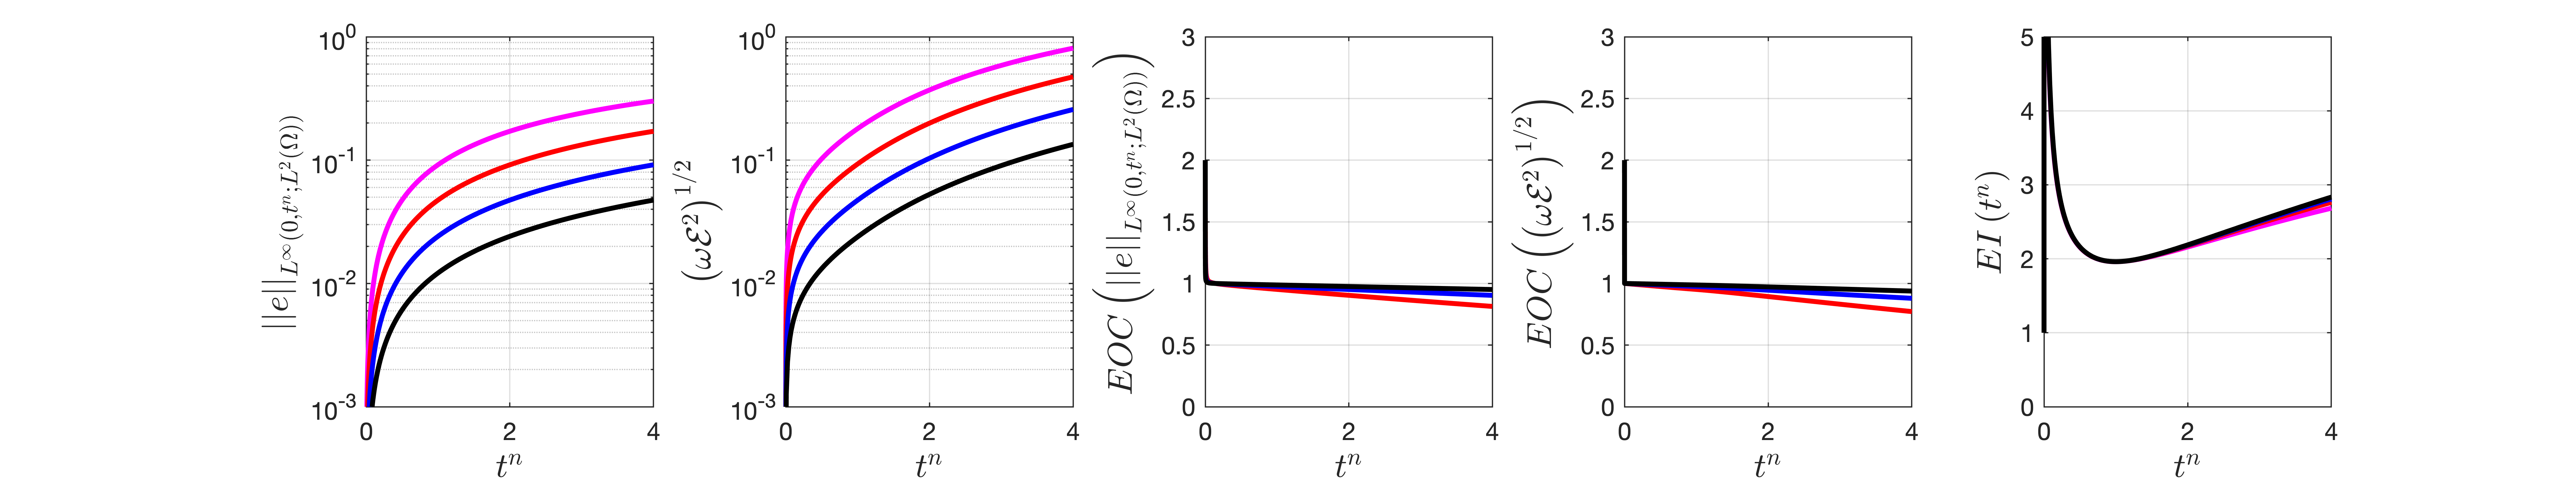
\includegraphics[width=\textwidth]{../figures/fig_FTBSplots_1x5_sin_IC_ind_uniform_P1}	
		\caption{
			\label{sfig:FTBS_prelim}
			FTBS (\ref{eq:FTBS}).
		}
	\end{subfigure}
	\\
	\begin{subfigure}[b]{\textwidth}
		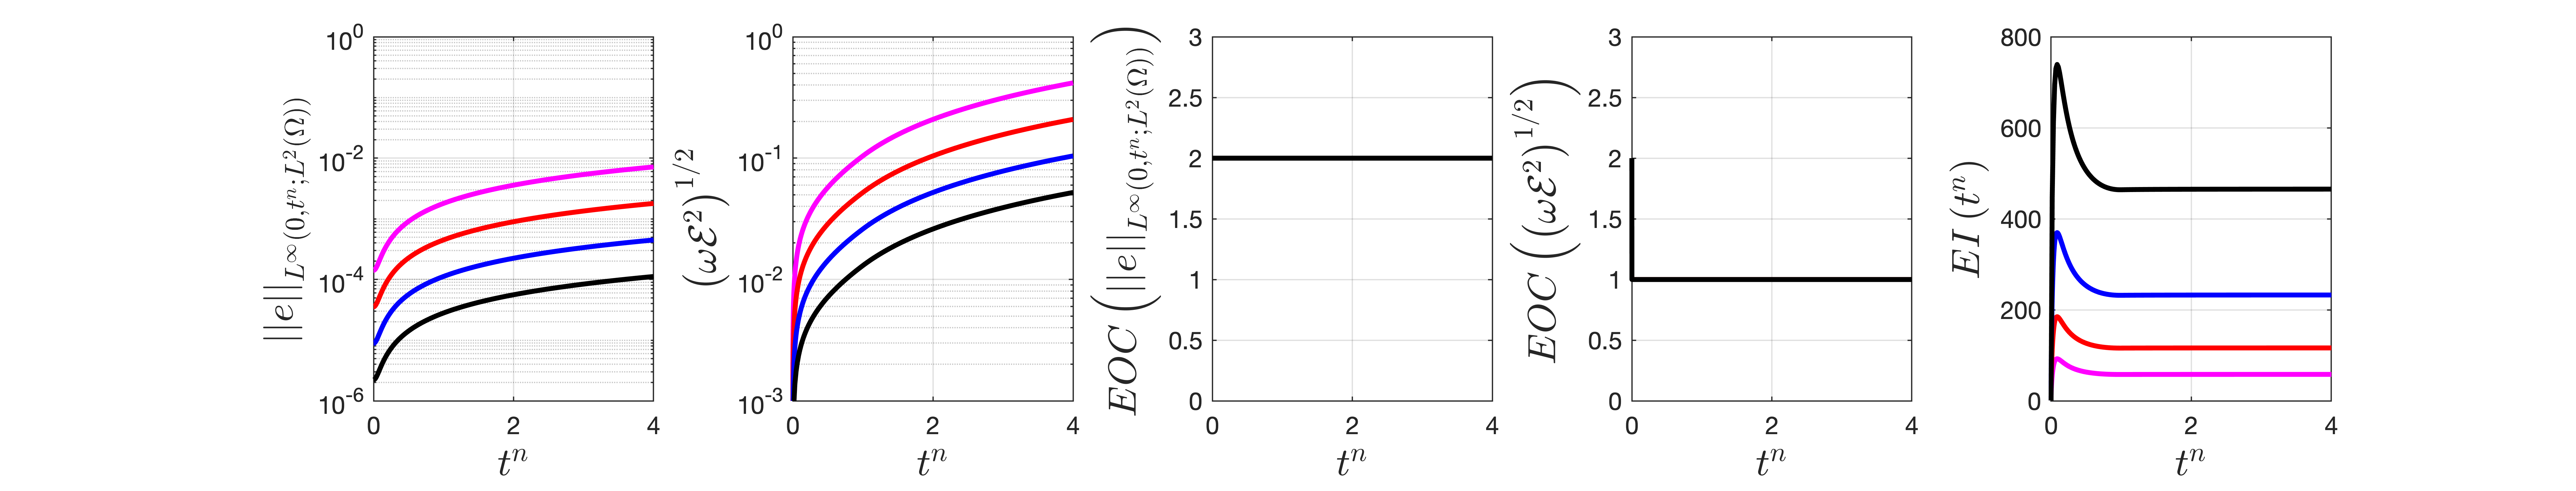
\includegraphics[width=\textwidth]{../figures/fig_CNCS_plots_1x5_sin_IC_ind_uniform_P1}	
		\caption{\label{sfig:FTCS_prelim_P1}
			CNCS (\ref{eq:FTCS}).
		}
	\end{subfigure}
	\caption{\label{fig:bilinearLagrange} Errors and asymptotic
          convergence rates for the bilinear interpolant of FTBS
          (\ref{eq:FTBS}) and CNCS (\ref{eq:FTCS}) approximations of
          (\ref{eq:transport}) with initial condition
          (\ref{eq_ic_sin}) and periodic boundary conditions. The
          simulations were conducted over a family of meshes with
          discretisation parameter $h = 2^{-m}, m = 4,\dots 7$, with a
          timestep $\tau = \tfrac{h^2}{10}$. Note that the estimate is
          optimal for the FTBS scheme and achieves a very favourable
          effectivity of $EI \qp{4} < 3$, however it is suboptimal for
          the CNCS scheme.  }
\end{figure}

The suboptimality in the a posteriori bound for the CNCS scheme can be
circumvented. We do this by building information from within the
finite difference spatial discretisation directly into the
post-processor. Indeed, augmenting $\widehat U$ such that it is
defined as the piecewise linear Lagrange interpolant of the finite
difference coefficients $\{U^n_j\}$ in time and the unique piecewise
quadratic interpolant satisfying
\begin{equation}
  \label{eq:quadrecon}
\begin{split}
\widehat U(x_j,t^n) &= U^n_j
\\
\widehat U(x_{j+1},t^n) &= U^n_{j+1}
\\
\partial_x \widehat U(x_j, t^n) &= \frac{U^n_{j+1}-U^n_{j-1}}{2h}
\end{split}
\end{equation}
we are closer to the spirit of a finite difference method. The
argument from Lemma \ref{subsec:asymptotic_convergence_rate} can be
modified to apply in this case. Indeed, one can show that applying the
same argument the interpolant given by (\ref{eq:quadrecon}) yields
$\sqrt{w\cE^2} = \Oh\qp{\tau^2+h^2}$, which is optimal for the CNCS
scheme. To illustrate this asymptotic convergence properties we have
replicated the same experiment as in Figure \ref{fig:bilinearLagrange}
for the quadratic reconstruction. This is shown in Figure
\ref{fig:FTCS_prelim_P2}.  It can be seen that the additional
information provided by appropriately increasing the order of data
representation allows us to achieve optimal convergence rates of the a
posteriori bound and favourable effectivities.

\begin{figure}[H] 
	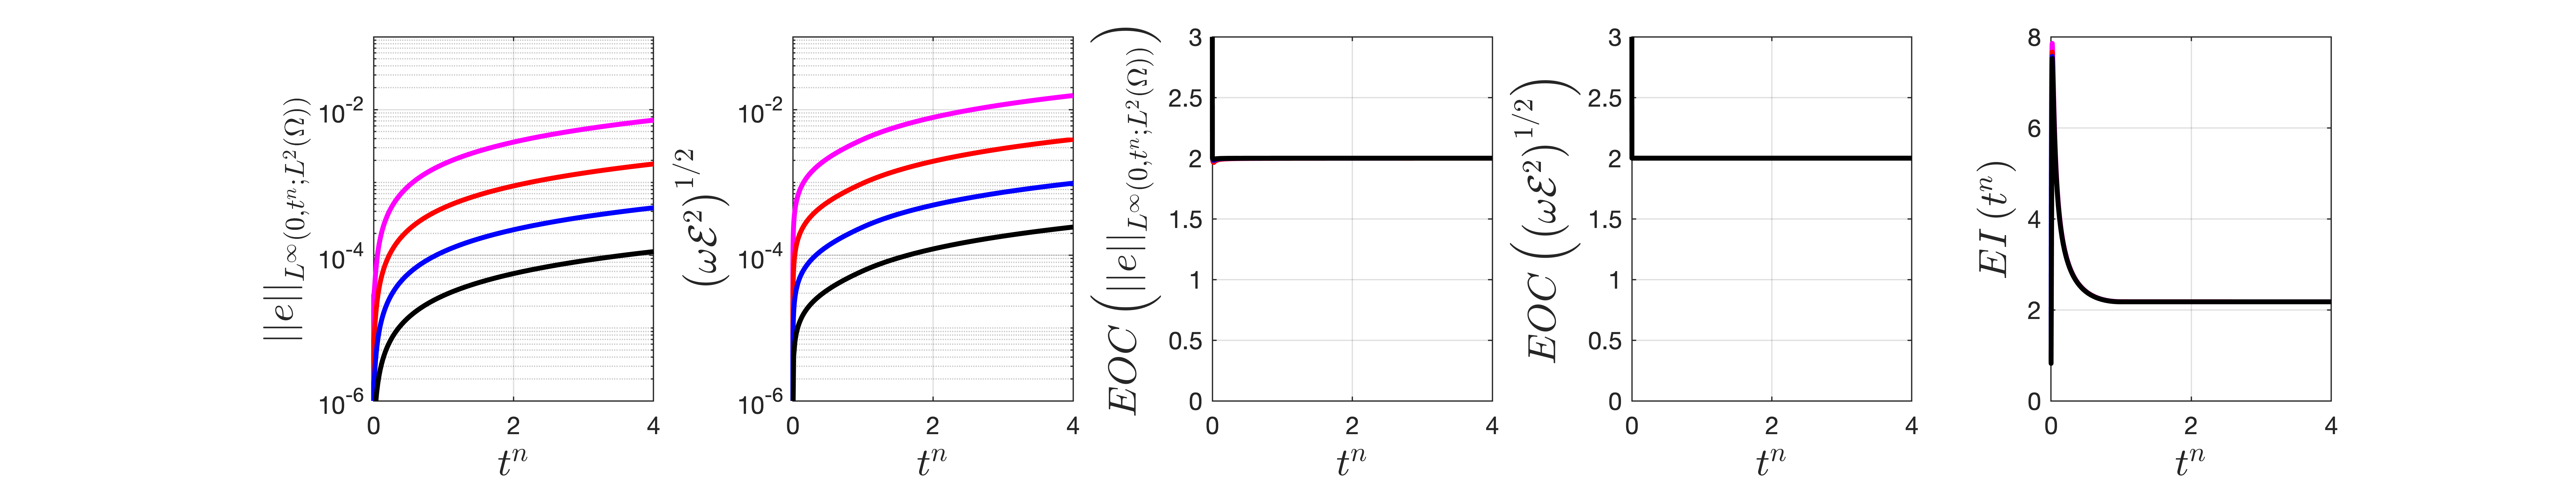
\includegraphics[width=\textwidth]{../figures/fig_CNCS_plots_1x5_sin_IC_ind_uniform_P2}	
	\caption{
		\label{fig:FTCS_prelim_P2}
		Errors and asymptotic convergence rates for the linear in time,
		quadratic in space Hermite interpolant of CNCS (\ref{eq:FTCS})
		approximations of (\ref{eq:transport}) with initial condition
		(\ref{eq_ic_sin}) and periodic boundary conditions. The simulations were conducted over a family of
		meshes with discretisation parameter $h = 2^{-m}, m = 4,\dots 7$,
		with a time-step $\tau = \tfrac{h}{10}$. Note that the estimate
		is now optimal for the CNCS scheme with favourable effectivity of
		$EI \qp{4} \sim 2.2$.}
\end{figure}

The ideas presented in this section form an intuitive way to obtain
the reconstruction. It is possible to generalise this quite naturally
to other spatio-temporal discretisations as we will present in the
forthcoming sections.

\section{General Systems}\label{sec:numerical_discretisation}

%% \begin{Rem}[Order of the methods]
%%   Note that the FTBS is formally order 1 in space and time. The FTCS
%%   method we write is formally order 1 in time and order 2 in space, even on a non-uniform grid.  Notice that on a
%%   uniform mesh the method simplifies to the more recognisable form
  %\begin{equation}
  %%   \begin{split}
  %%     U^{n+1}_j &= U^n_j + \tau^n\bigg(
  %%     \qp{\frac{1}{h_{j+1}} - \frac{1}{h_j+h_{j+1} } }U^n_{j+1} 
  %%     \\
  %%     &\qquad +
  %%     \qp{\frac{1}{h_{j}} - \frac{1}{h_{j+1} } }U^n_{j} +
  %%     \qp{\frac{1}{h_j+h_{j+1} } -\frac{1}{h_{j}} }U^n_{j-1}\bigg)
  %%     \text{ for } n=1,\dots, N \text{ and } j=1,\dots, M-1
  %%     \qp{U^n_{j+1}-U^n_{j-1}}
  %%     \text{ for } n=0,\dots, N-1 \text{ and } j=1,\dots, M-1.
  %%   \end{split}
  %% \end{equation}
%\end{Rem}


In this section we present spatial and temporal discretisations for schemes for more general conservation laws than in \S\ref{sec:example_aposteriori_bounds}.  Since we consider vectorial problems, we will denote by $\vec{U}^n_j$ the numerical approximation to $\vec u\qp{x_j, t^n}$.  
\begin{Rem}[One-dimensional system of conservation laws] We consider problems of the form
	\begin{equation}\label{eq_1d_gen_cons_law}
	\begin{aligned}
	\vect{u}_t+\partial_x\vect{f\qp{\vect{u}}}&=\vect{0},\\
	\vect{u}\qp{x,0}&=\vect{u}_0\qp{x},
	\end{aligned}\quad \text{ for } \qp{x,t}\in \W\times\qp{0,\infty}
	\end{equation}
	with $\vect{u}=\qp{u_1,\dots,u_p}^T$ and $\vect{f}\qp{\vect{u}}=\qp{f_1\qp{\vect{u}},\dots,f_p\qp{\vect{u}}}^T$ and complemented with periodic boundary conditions.
	In particular,
	\begin{equation}
	\dfunkmapsto{\vec{u}}{\mathbb{R}\times\mathbb{R}^+}{\mathbb{R}^p}{\qp{x,t}}{\vect{u}\qp{x,t}}
	\end{equation}
	and the flux function $\vect{f}$
	\begin{equation}
	\dfunkmapsto{\vec{f}}{\mathbb{R}^p}{\mathbb{R}^p}{\vect{u}\qp{x,t}}{\vect{f}\qp{\vect{u}\qp{x,t}}}
	\end{equation}
\end{Rem}

\begin{Defn}[Entropy/entropy-flux pair]
	The pair $\qp{\eta, q}$ is an entropy/entropy-flux pair associated with the conservation law (\ref{eq_1d_gen_cons_law}) iff $\eta$ is convex and
	\begin{equation}
	\D q= \D\eta \D f.
	\end{equation}  
\end{Defn}

\begin{Defn}[Entropy solution]
	A function $\vec{u}\in\leb{\infty}\qp{\mathbb{R^d}\times\qb{  0,\infty}}$ is an entropy solution of
	(\ref{eq_1d_gen_cons_law}) with an associated
	entropy/entropy-flux pair $\qp{\eta,q}$ if
	\begin{equation}
	\begin{aligned}
	\int_0^{\infty}\int_\Omega\vec{u}\cdot \partial_t \phi +\vec{f}\qp{\vec{u}}\cdot \partial_x\phi\, \mathrm{d}x\mathrm{d}t
	+\int_\Omega \vec{u}_0\cdot \phi \qp{\cdot,0} \mathrm{d}x& =0 \quad
	\forall\phi \in C^1_0\qp{\reals\times [0,\infty)}\quad\text{and}\\
	\int_0^\infty \int_\Omega \eta \qp{\vec{u}}\partial_t \phi + q\qp{\vec{u}}\partial_x \phi\, \mathrm{d}x\mathrm{d}t
	+ \int_\Omega \eta \qp{\vec{u}_0}\phi\qp{\cdot,0} \mathrm{d}x&\geq 0\quad \forall \phi \in C^1_c\qp{\reals \times [0,\infty)}
	\end{aligned}
	\end{equation}
	
	%	\begin{equation}
	%	\int_{\mathbb{R}^d}\int_{\mathbb{R}^+}\qp{S\qp{u}\partial_t\phi +F_S\qp{u}\cdot\nabla \phi}\mathrm{d}t
	%	\mathrm{d}x+\int_{\mathbb{R}^d}S\qp{u_0}\phi\qp{x,0}\mathrm{d}x\geq 0 \quad \forall \phi \in C^1_0\qp{\mathbb{R}^d\times\mathbb{R}^+,\mathbb{R}^+}
	%	\end{equation}
\end{Defn}
It can be verified that strong solutions of (\ref{eq_1d_gen_cons_law}) also satisfy the additional conservation law
\begin{equation}\label{eq_associated_cons_law}
\partial_t {\eta}\qp{\vec{u}} + \partial_x {q}\qp{\vec{u}} = 0.
\end{equation}
\subsection{Spatial discretisation}
It is well known that numerical schemes for
non-linear conservation laws may converge to functions which are not weak-solutions of the original problem (see \cite[\S12.1]{leveque1992numerical}). We address this problem by expressing the method in conservation form. We use a consistent numerical flux
function $\vec{F}$, which takes $p+q+1$ arguments:
\begin{equation}\label{eq_defn_num_flux}
\dfunkmapstonumflux{\qp{\vec{U}^n_{j-p+1},\cdots,\vec{U}^n_{j+q}}}{\vec{F}^n_j}{{\vec{F}}\qp{\vec{U}^n_{j-p},\cdots,\vec{U}^n_{j+q}}}{\vec{F}\qp{\vec{v},\cdots,\vec{v}}}{\vec{f}\qp{\vec{v}}, }
\end{equation}
where $p$ and $q$ are simply used to determine the width of the
computational stencil.  We use $\vec{F}$ to approximate
$\partial_{x}\vec{f}$ such that
\begin{equation}\label{eq_num_approx_f}
  \partial_{x}\vec{f}\qp{\vec{u}}\approx \frac{1}{h}\qp{{\vec{F}\qp{\vec{U}^n_{j-p},\cdots,\vec{U}^n_{j+q}}}-{\vec{F}\qp{\vec{U}^n_{j-p-1},\cdots,\vec{U}^n_{j+q-1}}}}.
\end{equation}
We can then use a method-of-lines approach in the discretisation of
(\ref{eq_1d_gen_cons_law}) by requiring
\begin{equation}\label{eq_conservation_form}
\frac{\mathrm{d}}{\mathrm{d}t}\vec{U}_j =  \frac{1}{h}\qp{{\vec{F}\qp{\vec{U}^n_{j-p},\cdots,\vec{U}^n_{j+q}}}-{\vec{F}\qp{\vec{U}^n_{j-p-1},\cdots,\vec{U}^n_{j+q-1}}}} \Foreach j=0, \dots, M.
\end{equation}
For clarity, we provide illustrative examples of $\vec{F}$ for the
Lax-Friedrichs and the Lax-Wendroff scheme. 

\begin{Rem}[Conservation form for the Lax-Friedrichs scheme]
  The Lax-Friedrichs scheme can be written in conservation form,
  (\ref{eq_conservation_form}), by defining the numerical flux
  function $\vec{F}$ as
  \begin{equation}\label{eq_F_LxF_cons}
     \vect F\qp{ \vect U_j,  \vect U_{j+1}}
    :=
    \frac{h}{2\tau}\qp{ \vec U_j- \vec U_{j+1}}
    +
    \frac{1}{2}\qp{ \vec f\qp{ \vec U_j}+ \vec f\qp{\vect U_{j+1}}}.
  \end{equation}
  %% The conservation form of the scheme is given by combining
  %% (\ref{eq_F_LxF_cons}) with a forward time-discretisation:
  %% \begin{equation}\label{eq_LxF_scheme}
  %%   U^{n+1}_j:= U^n_j-\frac{\tau}{h}\qp{F\qp{U^n_j, U^n_{j+1}}-F\qp{U^n_{j-1}, U^n_{j}}}.
  %% \end{equation}
  The Lax-Friedrichs flux is formally $\mathcal{O}\qp{h}$.
\end{Rem}

\begin{Rem}[Conservation form for the Lax-Wendroff scheme]
  The Lax-Wendroff scheme can be written in conservation form by
        using the Richtmayer two-stage method.  We define the numerical
        flux function $\vec F$ as
	\begin{equation}\label{eq_F_LxW_cons}
	\vec F\qp{\vec U_j,\vec U_{j+1}}:= \vec f\qp{\vec U^{n+1/2}_{j+1/2}},
	\end{equation}
	where 
	\begin{equation}
	\begin{split}
	\vec U^{n+1/2}_{j+1/2}&:=\frac{1}{2}\qp{\vec U^n_{j+1} + \vec U^n_{j}}-\frac{\tau}{2h}\qp{\vec f\qp{\vec U^n_{j+1}}-\vec f\qp{\vec U^n_j}}\\
	\vec U^{n+1/2}_{j-1/2}&:=\frac{1}{2}\qp{\vec U^n_{j} + \vec U^n_{j-1}}-\frac{\tau}{2h}\qp{\vec f\qp{\vec U^n_{j}}-\vec f\qp{\vec U^n_{j-1}}}.
	\end{split}
	\end{equation}
	The conservation form of the scheme is then given by:
	\begin{equation}\label{eq_LxW_scheme}
	\vec U^{n+1}_j:= \vec  U^n_j-\frac{\tau}{h}\qp{\vec f\qp{\vec U^{n+1/2}_{j+1/2}}-\vec f\qp{\vec U^{n+1/2}_{j-1/2}}}.
	\end{equation}
	The Lax-Wendroff scheme is formally $\mathcal{O}\qp{\tau^2 +h^2}$.
\end{Rem}


\subsection{Temporal discretisation}
We approximate the temporal variable using both implicit and explicit
temporal discretisations.  For example, using various $1$-stage Runge-Kutta methods given by the Butcher tableau
\begin{equation}
  \begin{array}
    {c|c}
    \theta & \theta
    \\
    \hline
    & 1 
  \end{array}.
\end{equation}
We also make use of Strong-Stability Preserving
Runge-Kutta (SSPRK) methods (see \cite{gottlieb2001strong}).
\begin{equation}
  \begin{array}{c|ccc}0&0&0&0\\1&1&0&0\\1/2&1/4&1/4&0\\\hline &1/6&1/6&2/3\\\end{array}.
\end{equation}



\section{WENO Schemes}\label{sec:ENO_WENO_schemes}

In this section we briefly summarise the details behind Weighted Essentially Non-Oscillatory (WENO) schemes, (cf. \cite{jiang1996efficient}, \cite{shu1998essentially}), which pertain to our implementation.  ENO/WENO schemes have been used with great success in several areas and in particular in the discretisation of hyperbolic conservation laws and convection-diffusion equations (see e.g. \cite{shu2020essentially} for an overview).   

They have several features which contributed to their widespread success.  These include a mechanism of computational stencil construction that can achieve arbitrarily high accuracy in regions where the solution is smooth, essentially non-oscillatory behavior in the vicinity of discontinuities (no artificial, numerical overshoots and undershoots) and proven ability to simulate complex smooth solution structures (see \cite{shu1998essentially} for more details).  In the present work we only consider WENO schemes.

There are two, closely related procedures that we use in the context of WENO schemes: reconstruction and approximation. The reconstruction procedure is used to form $\vec{F}$ in the spatial discritization of (\ref{eq_num_approx_f}) while the approximation procedure is used to obtain the spatial component of the post-processor from Lemma \ref{theorem_stab_advection} (see \S\ref{sec:general_reconstructions}). 


\begin{Rem}
	In order to avoid cofusion, it is emphasized that the ENO/WENO reconstruction procedure, as that is defined in \cite{shu1998essentially}, refers to the procedure  used to formulate the ENO/WENO numerical scheme.
	The reconstruction procedure we have developed refers to the procedure used to obtain the post-processor which is subsequently used for a posteriori error computations.  
	
	The readers should note that this procedure, as well as the characteristics of the resulting reconstruction,  are built using information from the scheme and are therefore inherently linked with it.
\end{Rem}


\begin{Defn}[WENO reconstruction problem from \cite{shu1998essentially}]
	Given the cell averages of a function $v\qp{x}$:
	\begin{equation}
	\bar{v}_j:= \frac{1}{h_j}\int_{x_j}^{x_{j+1}} v\qp{\xi}\mathrm{d}\xi, \quad j=0,\dots,M-1,
	\end{equation}
	find a polynomial $p_j\qp{x}$ of degree at most $k-1$ for each cell $I_j$ such that it is a $k-th$ order accurate approximation to $v\qp{x}$ inside $I_j$:
	\begin{equation}
	p_j\qp{x} = v\qp{x} + \mathcal{O}\qp{h^k}, \quad x\in I_j, \quad j=0,\dots,M-1.
	\end{equation}
\end{Defn}
The procedure for obtaining the polynomial $p_j$ from $\bar{v}_j$ can
be found in \cite[Procedure 2.2]{shu1998essentially} and in
\cite[\S.2.2]{shu2020essentially}.  This procedure is used both for
finite volumes and for finite differences with a minor difference.  In
the context of finite volumes, we use the cell averages $\bar{v}_j$ to
obtain a high order approximation to $v$.  We then substitute this in
an expression for $\vec{F}$ to calculate the numerical flux. In
contrast, in the context of finite differences, the computational
variables are point values rather than cell averages. In this case, the values 
$\vec{f}\qp{\vec{U}_j}$, $j=1,\dots,M$, are used  to obtain a high-order accurate approximation to $\vec{F}$
and subsequently $\partial_x\vec{f}$ in (\ref{eq_defn_num_flux}) and
(\ref{eq_num_approx_f}).  This is the approach we will be using
throughout this work.

We present this procedure below for a uniform scheme for simplicity.
The reader should note that in the shallow water numerical experiment in
\S\ref{sec:adaptive_experiments}, the WENO scheme used is derived for
a non-uniform scheme over an adaptive grid.
As a result, all geometry-related quantities - such as the sub-stencil polynomials, the smoothenss indicators and the resulting weights - are no longer pre-computable constants.  Instead, they have to be re-computed at every time-step.
The reader can find the detailed procedure on how to
derive the scheme on a non-uniform grid in \cite{shu1998essentially}.

\begin{Rem}[Order of WENO schemes on non-uniform grids]
	The reader is advised that, as is pointed out in
	\cite{shu1998essentially}, WENO schemes for finite differences which
	are posed on non-uniform grids cannot be higher than order
	two.
\end{Rem}


\subsection{The WENO-3 scheme}\label{subsec:WENO-3} In one spatial dimension, the WENO reconstruction procedure for the third order finite difference WENO scheme is used to approximate  $\vect f_x$ on the cell $I_j:=\qb{x_j, x_{j+1}}$.  The cell $I_j$ is chosen to be the central cell of the computational stencil $S:=\bracegs{I_{j-1}, I_j, I_{j+1}}$.  The approximation is then obtained as a convex combination of polynomials over two sub-stencils of $S$, namely 
\begin{equation}
\begin{aligned}
S_1&:=\bracegs{I_{j-1}, I_j}\quad \text{and}\\
S_2&:=\bracegs{I_{j}, I_{j+1}}.
\end{aligned}
\end{equation}
The polynomials $p_1\qp{x}$and
$p_2\qp{x}$ are the ENO reconstructions of $f\qp{u}$
on the substencils $S_1$ and $S_2$
respectively.  The numerical flux at $x_{j}$, denoted by
$F_{j}$, is obtained as the combination
\begin{equation}\label{eq_f_WENO}
F_{j}:=w_1p_1\qp{x_{j}} +w_2p_2\qp{x_{j}},
\end{equation}
where $w_1$ and $w_2$ are the non-linear weights (see (\ref{eq_non_lin_weights})) corresponding to $S_1$and $S_2$, which have to satisfy the conditions
\begin{equation}
w_l\geq 0,\quad \sum_{l=1}^2 w_l = 1.
\end{equation}
Finally, the WENO approximation to the flux derivative is obtained using
\begin{equation}\label{eq_WENO_approx_flux_derivative}
\partial_x f\simeq \frac{1}{h_{j-1}}\qp{F_{j}- F_{j-1}}.
\end{equation}


\begin{Rem}[Flux-splitting] When WENO schemes are implemented using finite differences one should ensure upwinding and stability (see \cite{shu1998essentially}).  This can be achieved in various ways.  In this paper, this was done by applying the chosen finite difference method to a \textit{flux-splitting} $f^{\pm}\qp{u}$ of $f\qp{u}$.  In particular, 
	\begin{equation}
	f\qp{u}= f^+\qp{u} + f^-\qp{u}.
	\end{equation}
	where 
	\begin{equation}
	\frac{d}{du}f^+\qp{u} \geq 0 \quad \text{and}\quad \frac{d}{du}f^-\qp{u} \leq 0.
	\end{equation}
	A simple flux-splitting is the Lax-Friedrichs splitting, which is given by 
	\begin{equation}
	f^{\pm}\qp{u}:=\frac{1}{2}\qp{f\qp{u}\pm \alpha u},
	\end{equation}
	For 1D scalar conservation laws
	\begin{equation}
	\alpha:=\max_{u}\norm{f'\qp{u}}.
	\end{equation}
	For hyperbolic systems of conservation laws, ${f}'$ is a Jacobian (with real eigenvalues).  In this case  upwinding is slightly more involved.  The reader should note that in that case one can either perform a characteristic decomposition (which is the more robust approach) or use flux-splitting on a component-by-component basis.  We opt for the latter route as it is sufficient for the purposes of this study.  In this case, $\alpha$ is calculated using the eigenvalues, $\lambda_i$, of the Jacobian ${f}'$:
	\begin{equation}
	\alpha := \max_{u} \max_{i} \abs{\lambda_i\qp{u}}.
	\end{equation}
	The reader should also note that when coding WENO schemes,  the stencil used for $f^+\qp{u}$ is biased to the left, while the stencil for $f^-\qp{u}$ is biased one point to the right. 
\end{Rem}
We will demonstrate the process for obtaining $f^+$ as an example. The
ENO sub-stencil polynomials for $f^+$, for a third order WENO scheme
are given by
\begin{equation}
\begin{aligned}
p_1\qp{U} &= \frac{1}{2}\qp{-f\qp{U_{j-1}} + 3f\qp{U_j}},\\
p_2\qp{U} &= \frac{1}{2}\qp{f\qp{U_{j}} + f\qp{U_{j+1}}}
\end{aligned}
\end{equation}
Next, we construct the weights $w_1$ and $w_2$.  Suppose
we wanted to create a reconstruction for a function $v\qp{x}$, which
is piecewise smooth in sub-stencils $S_1$ and $S_2$.  There are
constants $d_r$, $r=1,\,2$ such that
\begin{equation}
v_{j+1}=d_1v_{j+1}^{\qp{1}} +d_2v_{j+1}^{\qp{2}}=v\qp{x_{j+1}}+\mathcal{O}\qp{h^{2k-1}},
\end{equation} 
where $v^{\qp{i}}_{j+1}$ is the reconstruction of $v\qp{x}$ in the sub-stencil $S_i$ evaluated at $x_{j+1}$.  More specifically, for $f^+$,
\begin{equation}
d_0 = \frac{1}{3},\quad d_1=\frac{2}{3}.
\end{equation}
If $v\qp{x}$ is smooth, the nonlinear weights $w_i$ should
be very close to $d_i$.  If, instead, $v\qp{x}$ has a discontinuity in some
stencil, the $w_i$ from that stencil should be close to zero to avoid spurious oscillatory behaviour.
This is accomplished by using smoothness indicators $\beta_i$, where
\begin{equation}
\beta_i:=\sum_{l=1}^{k-1}\int^{x_{j+1}}_{x_j}h^{2l-1}\qp{\frac{\partial^lp_i\qp{x}}{\partial x^l}}^2\mathrm{d}x.
\end{equation}
This is simply a sum of scaled $\leb2$ norms of the derivatives of $p_i$.  The factor $h^{2l-1}$ ensures that $\beta_i$ scales like an $\leb{2}-$norm over polynomials. In the case of the third order WENO scheme over a uniform grid, 
\begin{equation}
\beta_1=\qp{v_{j-1}-v_j}^2,\quad \beta_2=\qp{v_j-v_{j+1}}^2.
\end{equation}
We can now obtain the weights $w_i$, which are given by
\begin{equation}\label{eq_non_lin_weights}
w_i:=\frac{\alpha_i}{\sum_{s=0}^{k-1}\alpha_s},  \text{ with  }\alpha_i = \frac{d_i}{\qp{\epsilon +\beta_i}^2}.
\end{equation}
The constant $\epsilon \ll 1$ is a small constant to ensure the
denominator does not vanish.  In experiments we use
$\epsilon=10^{-6}$.  We repeat this process to obtain $f^-$ noting
that in this case the entire computational stencil is biased one
position to the right.


\begin{Rem}[Choice of nonlinear weights]
	The choice of nonlinear weights is very important.  As is
	demonstrated in \cite{jiang1996efficient}, an appropriate choice of
	nonlinear weights can upgrade the order of accuracy of
	(\ref{eq_f_WENO}) in smooth regions relative to an ENO scheme with a stencil $S_1$ or $S_2$.  Furthermore, because these weights are
	designed to reflect the smoothness of the reconstruction polynomial
	in the relevant stencil, they are also used to facilitate the
	non-oscillatory property of the WENO scheme.  
	
	The Smoothness Increasing Accuracy Preserving (SIAC) filtering is a comparable concept.  This is a post-processing technique which has been used to reduce error oscillations and recover smoothness in the solution and its derivatives in the context of the Discontinuous Galerkin method (see \cite{dedner2019residual}).
\end{Rem}


\section{General reconstructions}\label{sec:general_reconstructions}

In this section we formally define a reconstruction and describe properties we would like it to possess.  Furthermore, we present a
methodology to obtain a space-time reconstruction from a computed
numerical solution for (\ref{eq_1d_gen_cons_law}).  We conclude the
section by illustrating the procedure of obtaining the spatio-temporal reconstruction from the numerical solution.

\begin{Defn}[Reconstruction]\label{defn_reconstruction}
The reconstruction, $\recgs{U}$, of the numerical solution, $\vec{U}$, to (\ref{eq_1d_gen_cons_law}) is a function that satisfies 
\begin{equation}
\label{eq:ibvpU}
\begin{aligned}
\widehat{\vect{U}}_t+\partial_x\vect{f\qp{\widehat{\vect{U}}}}
&=:-\vect{R}\quad \text{ in }\W \times (0,T]
\\
\widehat{\vect{U}}(\vect x,0) &= \vect{u}_0(\vect x) \quad \text{ in } \W \times \{0\}
\end{aligned}
\end{equation}
and periodic boundary conditions, such that the reconstruction residual, $\vect{R}$, is well-defined and
explicitly computable.  Furthermore,
$\widehat{\vect{U}}$ should lead to an optimal a posteriori
error estimate.  An estimate
is optimal when it converges at the same rate as the chosen numerical
scheme.
\end{Defn}



\/*

 The  reconstruction is a continuously defined object, obtained by applying an appropriate operator to the numerical solution. We will use in the calculation of $R$ in the bound in Lemma \ref{theorem_stab_advection}.  As such, it must satisfy certain properties to ensure that the bound  is optimal.  Interested readers can consult \cite[\S2]{makridakis2007space} for situations where the use of a reconstruction is preferrable to that of the numerical solution and potentail desirable characteristics for the reconstructions.  We will briefly summarise these.
Let $\vect u$ be an exact solution to an evolution problem $B\qp{\vect u}=0$, where $B$ is the PDE operator and consider a discrete approximation $B_h\qp{\vect U}=0$, where $\vect U$ is the numerical solution.  The form of $\vect U$ depends on the chosen numerical method and in the case of finite difference methods it is only defined pointwise. In constrast $\vect u$ is a continuously defined object.

The fact that $\vect U$ is only defined pointwise while $\vect u$ is defined continuously makes it is difficult to compute  quantities like $\Norm{\vect u-\vect U}_{\leb{p}\qp{\W}}$ or $\Norm{\vect U}_{\leb{p}\qp{\W}}$.  Such quantities are used in error estimation and are often required to implement adaptivity (see \cite{giesselmann2015posteriori}, \cite{giesselmann2017posteriori}).   These difficulties can be addressed by using  a reconstruction of $\vect U$, which we will denote by $ \widehat{\vect U}$.  This can be constructed such that it is not only continuously defined but to also possess an appropriate degree of smoothness.  
\begin{Rem}[Desirable characteristics for the reconstruction, $\widehat{\vect U}$, of $\vect U$]\label{rem_desirable_characteristics}Given a numerical solution $\vect U$ to (\ref{eq_cons_law_1D_discrete}), generated by a FD scheme, we would like  $\widehat{\vect U}$ to have the following properties:
	\begin{itemize}
		\item  $\Norm{\vect u-\widehat{\vect U}}_{\leb{p}\qp{\W}}$ should be computable or boundable by computable, optimal quantities \todo{what is optimal when the solution shocks? }.  Optimal quantities are those which converge with order at least equal to that of the FD scheme.
		\item The operator $B$ must be applicable to $\widehat{\vect U}$ i.e. $B\qp{\widehat{\vect U}}=R$ is computable explicitly.  Alternatively, it must be boundable by computable quantities.  We will refer to the  $R$ as the reconstruction residual.
		\item The reconstruction residual $R$ should be  both computable and optimal.  This is very important as this is the quantity that will be  eventually be used to bound the quantity $\Norm{\vect u-\widehat{\vect U}}_{\leb{p}\qp{\W}}$.
	\end{itemize}
\end{Rem}
*/


\subsection{Reconstruction Procedure} 
We obtain the polynomial reconstruction $\widehat{\vect U}$ by using the nodal values of $\vec{U}$ as
well as the temporal and spatial approximations of the partial
derivatives of the equation.  The reader should note that we
interpolate firstly in time and subsequently in space, because the
temporal component of (\ref{eq:ibvpU}) is linear while the spatial one
may be non-linear.

In the exposition that follows, we will use the superscripts $t$ and
$s$ to represent that the function in question is either time or space
dependent only.  We will also use the supercript $ts$ to denote
dependence on both time and space.

\begin{Defn}[Space of the spatial reconstruction step]
  Let $\polygsna{q}{\qb{x_j, x_{j+1}}}$ denote the space of
  polynomials of degree $q\in\mathbb{N}$ over the sub-interval
  $\qb{x_j, x_{j+1}}$.  We define the space of the spatial step of the
  reconstruction,
  \begin{equation}
    \mathbb{V}_q^s:=\bracegs{w:\qb{0,L}\rightarrow\mathbb{R}: w|_{\qb{x_j,x_{j+1}}}\in \polygsna{q}{\qb{x_j, x_{j+1}}}},
  \end{equation}
  to be the space of piecewise polynomials of degree $q$ over $\qb{0,L}$.  The superscript $s$ indicates the space dependence.
\end{Defn}

\begin{Defn}[Space of the temporal reconstruction step]
We define the space of the temporal step of
  the reconstruction as the space of piecewise polynomials of degree
  $r$ over $\qb{0,T}$ such that
  \begin{equation}
    \mathbb{V}_r^t\qp{{0,T};\leb{2}\qp{\Omega}}:=\bracegs{g:\qb{0,T}\rightarrow V: g|_{\qb{t^n, t^{n+1}}}\in \polygsna{q}{\qb{t^n, t^{n+1}},\leb{2}\qp{\Omega}}}.
  \end{equation}
  Here, $\polygsna{q}{\qb{t^n, t^{n+1}},V}$ is the space of functions which are polynomials of degree $q$ in time and belong to $V$ in space.
\end{Defn}

\begin{Defn}[Temporal reconstruction]\label{defn_temp_rec}
	The temporal reconstruction, $\widehat{\vec{U}}^t\in \mathbb{V}_r^t\qp{0,T;\mathbb{V}_q^s}$ of the numerical solution $\vect{U}$, is the unique function satisfying
	\begin{equation}\label{eq_conds_temp_rec}
	\begin{aligned}
	\widehat{\vec {U}}^t\qp{t^n}&={\vec{U}}^n_j\quad \text{and}\\
	\partial_t\widehat{\vec{U}}^t\qp{t^n}&=- \frac{1}{h}\qp{{\vec{F}\qp{\vec{U}^n_{j-p},\cdots,\vec{U}^n_{j+q}}}-{\vec{F}\qp{\vec{U}^n_{j-p-1},\cdots,\vec{U}^n_{j+q-1}}}}.
	\end{aligned}
	\end{equation}
	for $n=0,\dots,N$.  
\end{Defn}

\begin{Rem}[Order of the temporal reconstruction] The procedure presented in Defn. \ref{defn_temp_rec} limits the temporal component of the reconstruction to third order.  A possibility for increasing the order of the temporal reconstruction is by obtaining a WENO interpolant for the temporal component in the same way we will demonstrate for the spatial one in the following section.
\end{Rem}

Once we obtain the temporal reconstruction we use it to define the
full spatio-temporal reconstruction, which is used in all computations
involving the post-processor in Lemma \ref{theorem_stab_advection}.
The procedure used to obtain the spatial component is based on the
Weighted Essentially Non-Oscillatory (WENO) interpolation procedure
which is derived and presented in detail in \cite{janett2019novel}.

\subsection{WENO approximation}  In this section we present the procedure for obtaining the spatial component of the reconstruction using the WENO interpolation procedure of \cite{janett2019novel}. An advantage of this interpolant is that all its aspects (sub-stencil polynomials, linear and non-linear weights) have been modified for use on non-uniform grids.  In addition, it has the other advantages of WENO-interpolants.  These include high orders of approximation in regionwhere the solution is smooth and essentially non-oscillatory behavior in the vicinity of dicontinuities.  

Consider a function $y\qp{x}$ with a set of point values $\bracegs{y_j}$ at locations $\bracegs{x_j}$,  where  the grid is not necessarily uniform. We want to construct a third order WENO intepolating polynomial in an interval $\qb{x_j, x_{j+1}}$ by using the $4$-point stencil
\begin{equation}
S:=\bracegs{x_{j-1},\dots,x_{j+2}}
\end{equation}
 The interpolant is obtained as a convex combination of polynomials which are constructed on two 3-point sub-stencils, $S_1$ and $S_2$ of $S$, which are given by 
\begin{equation}
\begin{aligned}
S_1 &:= \braces{x_{j-1}, x_j, x_{j+1} },\\
S_2& :=  \braces{ x_j, x_{j+1} , x_{j+2}}.
\end{aligned} 
\end{equation} 
The polynomials are  Lagrange interpolants over the sub-stencils:
\begin{equation}
\begin{aligned}
p_1\qp{x}&:= y_{j-1}\frac{\qp{x-x_{j}}\qp{x-x_{j+1}}}{h_{j-1}\qp{h_{j-1}+h_j}} + 
                                y_{j}\frac{\qp{x-x_{j-1}}\qp{x-x_{j+1}}}{h_{j-1}h_j}  +
                                y_{j+1}\frac{\qp{x-x_{j-1}}\qp{x-x_{j}}}{\qp{h_{j-1}+h_j}h_j}\quad\text{and} \\
p_2\qp{x}&:= y_{j}\frac{\qp{x-x_{j+1}}\qp{x-x_{j+2}}}{h_{j}\qp{h_{j}+h_{j+1}}} + 
							  y_{j+1}\frac{\qp{x-x_{j}}\qp{x-x_{j+2}}}{h_{j}h_{j+1}}  +
							  y_{j+2}\frac{\qp{x-x_{j}}\qp{x-x_{j+1}}}{\qp{h_{j}+h_{j+1}}h_{j+1}}
\end{aligned}
\end{equation}
for $x\in \qb{x_j, x_{j+1}}$.  A  polynomial approximation to $u\qp{x}$, $p\qp{x}$, can be obtained as a convex combination of the $p^{\qp{i}}$.  The WENO approach is such that $p\qp{x}$ is a high order approximation in intervals where $u\qp{x}$ is smooth.  $p\qp{x}$ is obtained as a weighted sum of $p^{\qp{1}}$ with  the (linear) weights $\gamma_1$ and $\gamma_2$, each corresponding to a sub-stencil of the large stencil:
\begin{equation}
\begin{aligned}
\gamma_1\qp{x}&:= -\frac{x-x_{j+2}}{x_{j+2}-x_{j-1}}\quad\text{and}\\
\gamma_2\qp{x}&:= \frac{x-x_{j-1}}{x_{j+2}-x_{j-1}}.
\end{aligned}
\end{equation}
The linear weights are positive and satisfy 
\begin{equation}
\sum_i \gamma_i = 1.
\end{equation}
Interested readers can find details on the construction of these weights in (\cite{carlini2005weighted}) and \cite{liu2009positivity}.  If the solution is discontinuous inside a sub-stencil, we would like that stencil to have little contribution to ensure the non-oscillatory behaviour of the scheme.  This is achieved by using the non-linear weights $\w_i\qp{x}$, which are obtained from the $\gamma_i\qp{x}$ as follows:
\begin{equation}
\omega_j\qp{x}:=\frac{\alpha_j\qp{x}}{\sum_{i=1}^2\alpha_i\qp{x}},\quad \alpha_i\qp{x}:=\frac{\gamma_i\qp{x}}{\epsilon +\beta_i},
\end{equation}
where the $\beta_i$ are the \textit{smoothness indicators} for the sub-stencil to which they pertain.  They are an indication of how non-smooth the solution is in the corresponding sub-stencil.  If the solution is smooth in the sub-stencil $S_j$, then the relevant $\beta_j$ is small and the relevant $\omega_j$ is close to the $\gamma_j$ in $S_j$. If instead the solution has a discontinuity in $S_j$, then the $\beta_j$ is large, leading to a small $\omega_j$ and ensuring the non-oscillatory behaviour.

The $\beta_i$ which are used in this paper are given in \cite{janett2019novel} and are defined as
\begin{equation}
\begin{aligned}
\beta_1&:= \qp{h_j +h_{j+1}}^2\qp{\frac{\norm{y'_{j+1}-y'_j}}{h_j}  - \frac{\norm{y'_{j}-y'_{j-1}}}{h_{j-1}}}^2\quad \text{and}\\
\beta_2&:= \qp{h_{j-1}+h_{j}}^2\qp{\frac{\norm{y'_{j+2}-y'_{j+1}}}{h_{j+1}}  - \frac{\norm{y'_{j+1}-y'_{j}}}{h_{j}}}^2.
\end{aligned}
\end{equation}
The calculation of the $y'_i$ is presented in detail in \cite[\S3.3.2]{janett2019novel}.  Finally, the WENO approximation to $u\qp{x}$ in the interval $\qb{x_j, x_{j+1}}$ based on the stencil $S=S_1\cup S_2=\bracegs{x_{j-1}, x_j, x_{j+1}, x_{j+2}}$ can be obtained as
\begin{equation}\label{eq:weno_interpolant}
p\qp{x} := \w_1p_1\qp{x} + \w_2p_2\qp{x}.
\end{equation}
   Now we can define the spatio-temporal reconstruction in terms of the WENO approximation.


\begin{Defn}[Spatio-temporal reconstruction]\label{defn_spatio-temporal reconstruction}
	Let $ \widehat{\vec{U}}^t$ be a temporal reconstruction of the numerical solution $\vect{U}$ of (\ref{eq_1d_gen_cons_law}).  The spatio-temporal reconstruction $\widehat{\vec{U}}^{ts}\in\mathbb{V}^t_r\qp{0,T; \mathbb{V}^s_q}$ 
	in the interval $\qb{x_j, x_{j+1}}$ is given by the WENO interpolant of $\widehat{\vec{U}}^t$, which is defined in (\ref{eq:weno_interpolant}).
\end{Defn}
\/*
\subsection{WENO approximation}  The spatial component of the reconstruction is obtained using the WENO interpolation procedure of \cite{janett2019novel}.  An advantage of this choice compared to, say a  Lagrange/Hermite interpolant is that this smooth post-processor will have the ENO property, which is useful in the vicinity of discontinuities. Another important factor is that (in smooth regions) we can use this method to construct spatial post-processors of arbitrarily high order.  In contrast, a conventional Hermite interpolant would limit the post-processor to third order in light of the number of nodal and derivative conditions in the interval of consideration.  We summarise this procedure below.

Consider a function $y\qp{x}$ with a set of point values $\bracegs{y_j}$ at locations $\bracegs{x_j}$.  We define the WENO interpolant in $\qb{x_0, x_M}$ as the function
\begin{equation}\label{eq:WENO_interp}
W\qp{x}:= \sum_{j=0}^{M-1}p_j\qp{x}I_j\qp{x},
\end{equation}
where
\begin{equation}\label{eq:ind_function}
I_j\qp{x}:=\begin{cases}
1\quad \text{if } x \in \qb{x_j, x_{j+1}}\\
0 \quad \text{if } x \notin \qb{x_j, x_{j+1}}\\
\end{cases}
\end{equation}
and $p_j$ is the interpolating polynomial in the interval $\qb{x_j,x_{j+1}}$, which is a $p-th$ order approximation to $y\qp{x}$ in that interval, i.e.
\begin{equation}
p_j\qp{x} = y\qp{x} + \mathcal{O}\qp{\Delta x^p}, \quad \text{for } x\in \qb{x_j, x_{j+1}}.
\end{equation}
The polynomial $p_j$ is constructed on the $p$-point stencil, $S^q_p$, where $q\in\bracegs{1,\dots,p}$ and
\begin{equation}
S^q_p:=\bracegs{x_{j-p+q},\dots,x_{j+q-1}}
\end{equation}
The central idea behind this WENO approximation method is that $p_j$ is constructed  as a convex combination of $l$-th order  accurate ($l<q$) Lagrange polynomials, $q_m\qp{x}$.  The polynomials $q_m\qp{x}$ are constructed on $l$- point sub-stencils of $S^q_p$, which we will denote by $S^m_l$, with $l\in\bracegs{1,\dots,p}$ and $m\in\bracegs{-p+q+l,\dots,q}$.  The polynomial $p_i\qp{x}$ is recovered as a convex combination of the $q_m\qp{x}$ polynomials:
\begin{equation}
p\qp{x}:=\sum_{m=-p+q+l}^q\omega\qp{x}q_m\qp{x},
\end{equation}
 where the $\omega_m$ are called the \textit{non-linear} weights.  The success of the WENO schemes depends heavily on the appropriate choice of the $\omega_m$ (see \cite{shu1998essentially}. Interested readers can find more detailed discussions on the choice of weights in \cite{carlini2005weighted} and \cite{liu2009positivity}.  In this work, the weights are obtained as shown in \cite[\S3]{janett2019novel}.   Now that we have the defined the WENO approximation procedure, we can define the spatio-temporal reconstruction. 
 \/*

\begin{Defn}[Finite difference approximation of deratives of $\vect{u}$]
	We will use the notation 
	$\FD\qp{\vect{U}^n_j}$
	to denote the chosen finite difference approximation to $\partial_x\vect{u}\qp{x_j,t^n}$. As an illustrative example,  a central difference quotient in this notation could be defined as
	\begin{equation}
	\FD\qp{\vect{U}^n_j}:=\frac{\vect{U}^{n}_{j+1}-\vect{U}^{n}_{j-1}}{2\Delta x}.
	\end{equation}
\end{Defn}
\begin{Rem}[On the choice of $\FD$]
We choose the operator $\FD$  to be the same as RHS (\ref{eq_num_approx_f})  but with $\vec{f}\qp{\vec{u}}=\vec{u}$.  This is equivalent to the spatial discretisation for an advection equation for $\vec{u}$.
\end{Rem}

\begin{Defn}[Spatio-temporal reconstruction]
	Let $ \widehat{\vec{U}}^t$ be a temporal reconstruction of the numerical solution $\vect{U}$ of (\ref{eq_1d_gen_cons_law}).  The spatio-temporal reconstruction $\widehat{\vec{U}}^{ts}\in\mathbb{V}^t_r\qp{0,T; \mathbb{V}^s_q}$ is given by
	\begin{equation}
	\begin{aligned}
	\widehat{\vect {U}}^{ts}\qp{ x_j,t^n}&= 
	{ \widehat{\vect {U}}^t}_j\qp{t^n}\quad \text{and}\\
	\partial_{x}{ \widehat{\vect {U}}^{ts}\qp{ x_j,t^n}}&= 
	\FD{\qp{ \widehat{\vect {U}}^t_j  }}
	\end{aligned}
	\end{equation}
	for $n=0,\dots,N$ and $j=0,\dots,M-1$.  
\end{Defn}
*/

\/*
Next, we present how Defns. \ref{defn_temp_rec} and \ref{defn_spatio-temporal reconstruction} are used to obtain the reconstruction $\recgs{U}$ (equiv. $\recgs{U}^{ts}$).  We will do this by firstly obtaining $\recgs{U}^s$ and then using it to obtain $\recgs{U}$.
\begin{Rem}[Polynomial form of $\recgs{U}^t$] The conditions (\ref{eq_conds_temp_rec}) can be used to obtain $\recgs{U}$ as a polynomial in $\qp{t-t^n}$ for $t\in\qb{
	t^n, t^{n+1}}$ :
\begin{equation}
\widehat{\textbf {U}}^t\qp{t}:=\vect{c}_0 +\vect{c}_1\qp{t-t^n} +\vect{c}_2\qp{t-t^n}^2+\vect{c}_3\qp{t-t^n}^3,
\end{equation}
where the coefficients $\vect{c}_i$ are as follows:
\begin{equation}
\begin{aligned}
\vect{c}_{0} &= \vect{U}^n\\
\vect{c}_{1}&=-\vect{f}_h^n \\
\vect{c}_{2}&=\frac{1}{\Delta t}\qp{\vect{f}_h^{n+1}-\vect{f}_h^n}+\frac{3}{\Delta t^2}\qp{\vect{U}^{n+1}-\vect{U}^{n}+\Delta t \vect{f}_h^n}\\
\vect{c}_{3}&=-\frac{1}{\Delta t^2}\qp{\vect{f}_h^{n+1}-\vect{f}_h^n}-\frac{2}{\Delta t^3}\qp{\vect{U}^{n+1}-\vect{U}^{n}+\Delta t \vect{f}_h^n}\\
\end{aligned}
\end{equation}
\end{Rem}
\begin{Defn}[Polynomial form of $\recgs{U}$]\label{defn_spatio_temp_rec_shw}
	The spatio-temporal reconstruction can be obtained as a polynomial in $\qp{x,t}$ for $\qp{x,t}\in\qb{x-x_j}\times\qb{t-t^n}$,  using the conditions (\ref{eq_conds_spatiotemp}) and $\recgs{U}^t$:
	\begin{equation}
	\recgs{U}\qp{x,t}:=\vect{c}_0\qp{t} +\vect{c}_1\qp{t}\qp{x-x_j} +\vect{c}_2\qp{t}\qp{x-x_j}^2+\vect{c}_3\qp{t}\qp{x-x_j}^3,
	\end{equation}
	where the $\vect{c}_i\qp{t}$ are as follows:
	\begin{equation}
	\begin{aligned}
	\vect{c}_{0}\qp{t} &= {\recgs{U}}^t\qp{t},\\
	\vect{c}_{1}\qp{t}&=\FD\qp{\recgs{{U}}^t\qp{t}},\\
	\vect{c}_{2}\qp{t}&=-\frac{1}{\Delta x}\qp{\FD\qp{{\recgs{U}^t_{j+1}}\qp{t}}-\FD\qp{{\recgs{U}}^t_j\qp{t}}}+
	\frac{3}{\Delta x^2}\qp{ \recgs{{U}}^t_{j+1}\qp{t}- \recgs{{U}}^t_j\qp{t}-\Delta x\FD\qp{\recgs{{U}}^t_{j}\qp{t}}}\quad \text{and}\\
	\vect{c}_{3}\qp{t}&=\frac{1}{\Delta x^2}\qp{\FD\qp{\recgs{{U}}^t_{j+1}\qp{t}}-\FD\qp{\recgs{{U}}^t_{j}\qp{t}}}
	-\frac{2}{\Delta x^3}\qp{\recgs{{U}}^t_{j+1}\qp{t}-\recgs{{U}}^t_j\qp{t}-\Delta x \FD\qp{\recgs{{U}}^t_j\qp{t}}},\\
	\end{aligned}
	\end{equation}
	for $j=0,\dots,M$ or $j=0,\dots,M-1$ for periodic boundary conditions.
\end{Defn}
*/

\begin{Rem}[Order of the reconstruction]
	The conditions presented in Defn. \ref{defn_temp_rec} result in a polynomial which is of third order in the temporal variable.   In contrast Defn. \ref{defn_spatio-temporal reconstruction} can be used to obtain spatial reconstructions of arbitrary order in space, simply by using a higher order WENO interpolant.  The limiting factor in the oder of the full spatio-temporal reconstruction will be the lowest order between the spatial and temporal steps.  In this case, this will be the order of the temporal component (order three). 
\end{Rem}
\begin{Rem}[Boundary conditions]
Note that for periodic boundary conditions, quantities calculated in Defns. \ref{defn_temp_rec} and \ref{defn_spatio-temporal reconstruction} that pertain to the boundaries - i.e. $j=0$ and $j=M$ - should be equal.  In the case of non-periodic boundary conditions - Neumann boundary conditions in particular - the computational domain is extended using an appropriate number of ghost nodes.  For WENO schemes the number of ghost nodes depends on the WENO sub-stencil width.  The values for the ghost nodes can be obtained by extrapolation based on the local WENO polynomials.
\end{Rem}
 
We illustrate the reconstruction procedure in Fig. \ref{fig_spatiotemp_reconstruction}.  Firstly, we use Defn. \ref{defn_temp_rec} to obtain $\widehat{\vect {U}}^t\qp{t}$ from  $\vect{U}$, where the latter is produced by  the chosen numerical discretisation to (\ref{eq:transport}).  This is the solid red line in the middle plot.  Then, we use Defn. \ref{defn_spatio-temporal reconstruction} to obtain $\widehat{\vect {U}}^{ts}\qp{x,t}$ from $\widehat{\vect {U}}^{t}\qp{t}$.  This is the transparent red surface in the third plot. 

\/*
The first step is to obtain the temporal reconstruction,  $\widehat{\vect {U}}^t\qp{t}$, as a third order Hermit interpolant using  $\vect {U}^n$ and $\vect {U}^{n+1}$.  This is plotted as red lines in  Fig. \ref{fig_spatiotemp_reconstruction} (middle).  Firstly, we let
\begin{equation}
\widehat{\vect U}^t\qp{t}=\vect{c}_0 +\vect{c}_1\qp{t-t_n}+\vect{c}_2\qp{t-t_n}^2+\vect{c}_3\qp{t-t_n}^3
\end{equation}
and we use the conditions in Defn. \ref{defn_temp_rec}  to get the conditions the constant coefficients $c_i$:
\begin{equation}
\begin{aligned}
\recgs{U}^t\qp{t^n} &=\vect{U}^n,\\
\partial_t \widehat{\vect U}^t\qp{t^n}&=-\vect{f}^n_h,\\
\widehat{\vect U}^t\qp{t^{n+1}} &=\vect{U}^{n+1},\\
\partial_t \widehat{\vect U}^t\qp{t^{n+1}}&=-\vect{f}^{n+1}_h,
\end{aligned}\quad
\Rightarrow \quad 
\begin{aligned}
\vect{c}_0&=\vect U^n,\\
\vect{c}_1&=-\vect{f}_h^n,\\
\vect{c}_2&=\frac{3}{\Delta t^2}\qp{\vect U^{n+1}-\vect U^n}+\frac{1}{\Delta t}\qp{\vect{f}^{n+1}_h+2\vect{f}^n_h}\\
\vect{c}_3&=-\frac{1}{\Delta t^2}\qp{\vect{f}^{n+1}_h+\vect{f}^n_h}-\frac{2}{\Delta t^3}\qp{\vect U^{n+1}-\vect U^n}.\\
\end{aligned}
\end{equation}
Next, we use Defn  \ref{defn_spatio-temporal reconstruction} to obtain $\widehat{\vect U}^{ts}\qp{x,t}$ as another Hermite interpolant, only now we  use $\widehat{\vect U}^t$ instead of $\vect U$.  In this case, the $\vect{c}_i$ will depend on $\recgs{U}^t$ and will therefore be themselves time-dependent. We let
\begin{equation}
\widehat{\vect U}^{ts}\qp{x,t} =\vect{c}_0\qp{t}+\vect{c}_1\qp{t}\qp{x-x_j}+\vect{c}_2\qp{t}\qp{x-x_j}^2+\vect{c}_3\qp{t}\qp{x-x_j}^3
\end{equation}
and we use the conditions in Defn. \ref{defn_spatio-temporal reconstruction}  to obtain the time-dependent coefficients $\vect{c}_i\qp{t}$:
\begin{equation}
\begin{aligned}
\recgs{U}^{ts}\qp{x_j,t} &=\recgs{U}^t_j\qp{t},\\
\partial_x \recgs{U}^{ts}\qp{x_j,t}&=\FD\qp{\recgs{U}^t_j\qp{t}},\\
\recgs{U}^t\qp{x_{j+1},t} &=\recgs{U}^t_{j+1}\qp{t},\\
\partial_x \recgs{U}^{ts}\qp{x_{j+1},t}&=\FD\qp{\recgs{U}_{j+1}^t\qp{t}},
\end{aligned}\quad
\Rightarrow \quad 
\begin{aligned}
\vect{c}_0\qp{t}&=\recgs{U}_j^t\qp{t},\\
\vect{c}_1\qp{t}&=\FD\qp
\\{\recgs{U}_j^t\qp{t}},\\
\vect{c}_2\qp{t}&=\frac{3}{ \Delta x^2}\qp{\recgs{U}_{j+1}^t\qp{t}-\recgs{U}_j^t\qp{t}}
                -\frac{1}{\Delta x}\qp{\FD\qp{\recgs{U}_{j+1}^t\qp{t}}+2\FD\qp{\recgs{U}_j^t\qp{t}}},\\
\vect{c}_3\qp{t}&=\frac{1}{\Delta x^2}\qp{\FD\qp{\recgs{U}_{j+1}^t\qp{t}}+\FD\qp{\recgs{U}_j^t\qp{t}}}
                 -\frac{2}{\Delta x ^3}\qp{\recgs{U}_{j+1}^t\qp{t}-\recgs{U}_j^t\qp{t}}.\\
\end{aligned}
\end{equation}
$\widehat{\vect U}^{ts}\qp{x,t}$ is plotted as a red, transparent surface in Fig. \ref{fig_spatiotemp_reconstruction} (right).
*/
\begin{figure}[h]
	\centering
	\centering
	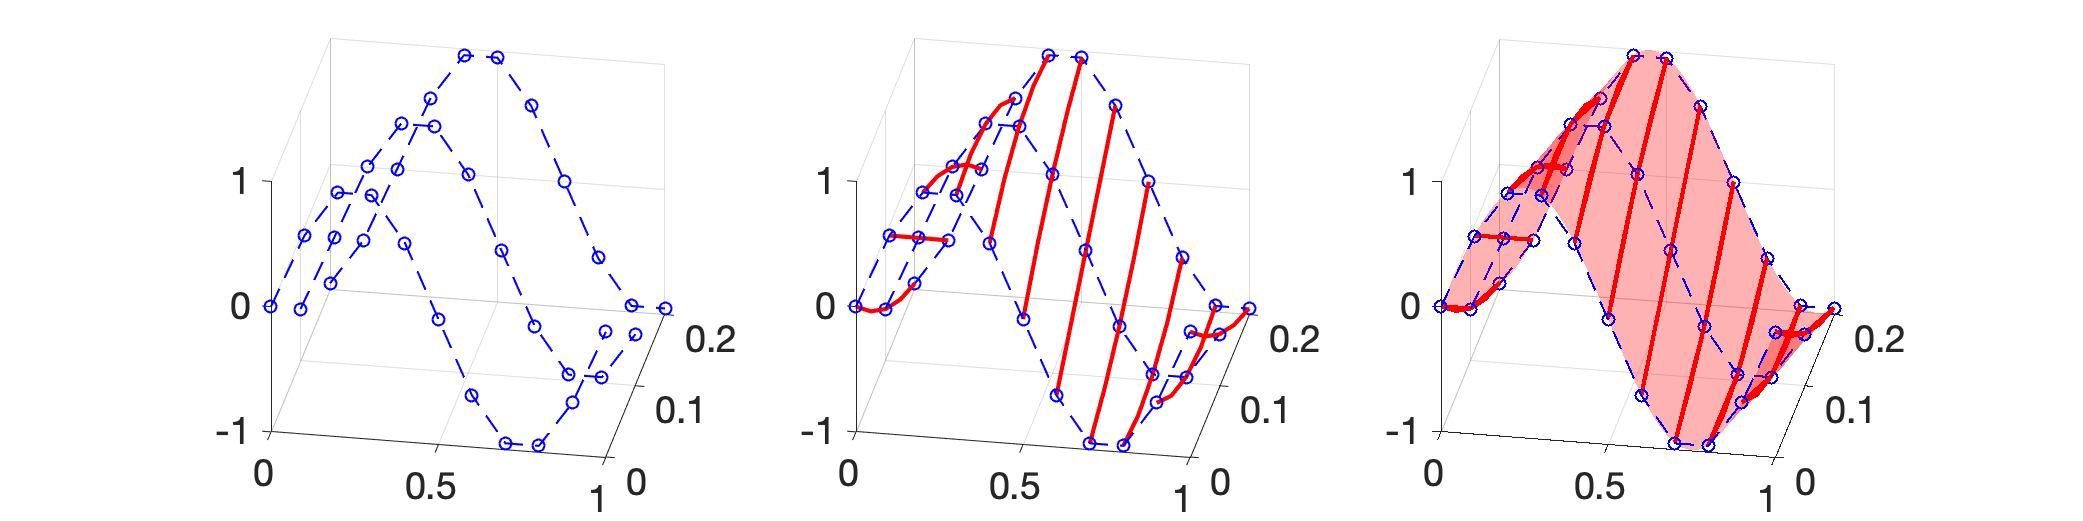
\includegraphics[scale=.5]{../figures/fig_P1_spatiotemp_1D}	
	\caption{Example of a reconstruction procedure.  (Left) $\vect{U}^n$ for $n=0,1,2$ produced by a Finite Difference scheme in 1D, with periodic boundary conditions and a sinusoidal initial condition (blue dashed lines).  (Middle) Temporal reconstruction step $\recgs{U}^t\qp{t}$, depicted as solid, red lines. (Right) Spatio-temporal reconstruction step $\recgs{U}^{ts}\qp{x,t}$, depicted as a transparent, red surface.  }
	\label{fig_spatiotemp_reconstruction}
\end{figure}

\section{Numerical verification}\label{sec:numerical_verification}
In this section we will study the asymptotic behaviour of the a
posteriori bound and compare and contrast it with the behaviour of the
error for two nonlinear examples: Burgers' equation and the shallow
water equations.  In both cases we are using periodic boundary
conditions.  The tests in this section are a preliminary step before
the next section, in which the a posteriori bound is used as a
refinement/coarsening criterion in adaptive tests.  We will firstly
present the bounds we will be testing for the non-linear problems we
benchmark in this section, along with the numerical schemes we will
use.
\begin{Rem}[a posteriori bound for nonlinear problems]
 The test cases we examine in this section are nonlinear so the
 post-processor from Lemma \ref{theorem_stab_advection} is not
 applicable.  Instead, we will use a different a posteriori estimate
 which is appropriate for nonlinear systems of hyperbolic conservation
 laws.
\end{Rem}
\/*
\begin{Lem}[Stability and error control for Burgers' equation]\label{theorem_stab_burgers}
Let $u\qp{x,t}$ be an entropy solution to the initial value problem 
\begin{equation}
\begin{aligned}
u_t+\partial_x\qp{\frac{u^2}{2}}&=0\\
u\qp{x,0}&=u_0\qp{x}
\end{aligned}
\end{equation}
with periodic boundary conditions and suppose $v$ is an entropy
solution of the perturbed problem for some $R \in \leb{\infty}(0,T;
\leb{2}(\W))$
\begin{equation}
\begin{aligned}
v_t+\partial_x\qp{\frac{v^2}{2}}&=-R\\
v\qp{x,0}&=v_0\qp{x}
\end{aligned}
\end{equation}
with periodic boundary conditions. Then, the error $e:=u-v$ satisfies
the following bound for all $t\in\qb{0,T}$:
\begin{equation}
\begin{aligned}
\Norm{e\qp{t}}^2_{L_2}\leq \exp\qp{\int_0^t\qp{\Norm{v_x\qp{s}}_{L_\infty}+1}\mathrm{d}s}\qb{\Norm{e\qp{0}}_{L_2}^2+\int_0^t\Norm{R\qp{s}}^2_{L_2}\mathrm{d}s}=: \cE_b^2\qp{t}.
\end{aligned}
\end{equation}
\end{Lem}
*/
\begin{Rem}[Reconstruction residual]\label{Rem_reconstruction_residual_eq_adv}
  The reconstruction residual, $\vect{R}$, is used to compute the smooth post-processor that bounds the error of the problem from above in Thm. \ref{theorem_stab_advection}.  We obtain $\vect{R}$ by substituting $\recgs{U}^{ts}$ in (\ref{eq_1d_gen_cons_law}):
	\begin{equation}\label{eq_reconstruction_gen_cons}
	-\recgs{R}\qp{ x,t}:=\partial_t\widehat{\vect U}^{ts}\qp{ {x},t}+\partial_x \vect{f}\qp{\recgs{U}^{ts}\qp{x,t}}
	\end{equation}
\end{Rem}

\begin{Rem}(Derivative notation)
We use the convention that derivatives of a vector-valued function $\vect{u}=\qp{u_1, \dots, u_d}^T$, are understood component-wise:
\begin{equation}
\partial_x \vect{u} := \qp{\partial_x u_1,\dots,\partial_x u_d}^T,
\end{equation}
where $\qp{\cdots}^T$ denotes a column vector.
Derivatives of a field, q, are denoted $\D q:=\qp{\partial_{u_1}q\qp{\vect{u}},\dots, \partial_{u_d}q\qp{\vect{u}}}$.  The matrix of second derivatives is 

\begin{equation}
	\D^2q\qp{\vec{u}}:=\begin{bmatrix}
\partial_{{u_1,}{u_1}}{q\qp{\vec{u}}}&\dotsc&\partial_{{u_1,}{u_d}}{q\qp{\vec{u}}}
\\
\vdots & \ddots &\vdots
\\
\partial_{{u_d,}{u_1}}{q\qp{\vec{u}}}&\dotsc&\partial_{{u_d,}{u_d}}{q\qp{\vec{u}}}
\end{bmatrix}.
\end{equation}
\end{Rem}
\begin{Lem}[a posteriori error control for nonlinear systems of 1D conservation laws from \cite{giesselmann2015posteriori}] \label{theorem_apost_control_nonlinear}Let $\vec{f}\in C^2\qp{U,\mathbb{R}^d}$ satisfy (\ref{eq_associated_cons_law}) and let $\vec{u}$ be an entropy solution of (\ref{eq_1d_gen_cons_law}) with periodic boundary conditions.  Let $\recgs{U}$ take values in $\mathcal{D}$ (which is a convex, compact subset of the state space).  Then for $0\leq t\leq T$ the error between $\vec{u}$ an  $\recgs{U}$ is given by 
\begin{equation}\label{eq_bound}
\begin{aligned}
\Norm{\vect{u}\qp{\cdot,t}-\recgs{U}\qp{\cdot,t}}^2_{\leb{2}\qp{I}}\leq&
\Cueta^{-1}\qp{\Norm{\vect{R}}^2_{\leb{2}\qp{I\times\qp{0,t}}}
  +\Coeta\Norm{\vect{u}_0-\recgs{U}_0}^2_{\leb{2}\qp{I}}}\\ &\times\exp\qp{\int_0^t\frac{\Coeta
    \Cof \Norm{\partial_x\recgs{U}\qp{\cdot,s}}_{\leb{\infty}\qp{I}}
    +\Coeta^2}{\Cueta}\mathrm{d}s}.
\end{aligned}
\end{equation}
The constants $\Cueta$ and $\Coeta$ represent the minimum and maximum absolute eigenvalues of $\D^2 \eta$. Furthermore, $\Cof:=\qp{\sum_i \Cofi}^{1/2}$, where $\Cofi$ is an upper bound for the absolute values of the eigenvalues of the \textit{i}th component of $\vec{f}$.
\end{Lem}

\begin{Cor}[Stability and error control for Burgers' equation with periodic boundary conditions]
	\label{cor_stab_control_burgers}
	Let the conditions of Lemma
        \ref{theorem_apost_control_nonlinear} hold with
        $f\qp{u}:=\frac{1}{2}u^2$, i.e. the scalar Burgers'
        equation. Suppose the initial value problems for $u$ and
        $v:=\widehat{U}$ are coupled with periodic boundary data.
        Then, the error between the two functions, $e:=
        u-\widehat{U}$, satisfies the following bound for all $t\in
        [0,T]$:
	\begin{equation}\label{eq:burgers_bound}
	\Norm{e\qp{t}}^2_{\leb{2}}\leq \exp\qp{\int_0^t\qp{\Norm{\partial_x\widehat{U}\qp{s}}_{\leb{\infty}}+1}\mathrm{d}s}\qb{\Norm{e\qp{0}}_{\leb{2}}+\int_0^t\Norm{R\qp{s}}^2_{\leb{2}}\mathrm{d}s}=: \w\qp{t}\cE_b^2\qp{t},
	\end{equation}
	where 
	\begin{equation}
-R:=\partial_t\widehat{U} +\partial_x\qp{\frac{\widehat{U}^2}{2}}.
	\end{equation}
\end{Cor}

We test the bound (\ref{eq:burgers_bound}) for three different schemes
- Lax-Friedrichs, Lax-Wendroff and SSP3-WENO - with uniform temporal
and spatial discretizations, i.e. $\tau^n:=\tau $ $\forall n$ and
$h_j:=h$ $\forall j$.  The reconstruction residual,
(\ref{eq_reconstruction_gen_cons}), will be obtained by using
Defn. \ref{defn_temp_rec} for the temporal component and
Defn. \ref{defn_spatio-temporal reconstruction} for the spatial
component.


We have implemented the a posteriori bound with these numerical
schemes in order to benchmark its behaviour before applying it to
adaptive scenarios, where the bound is used as a driver for
adaptivity.

\subsection{Test 1: Scalar Inviscid Burgers' equation. }
We will benchmark the performance of the a posteriori bound
(\ref{eq:burgers_bound}) in using the 1D inviscid Burgers' equation
with smooth a initial condition and periodic boundary conditions as
the test case:
\begin{equation}\label{eq_burgers}
\begin{aligned}
\partial_t u +\partial_x\qp{\frac{u^2}{2}}&=0,\\
u\qp{x,0}&=-\sin{x}
\end{aligned}\quad \text{for }\qp{x,t} \in \qb{-\pi,\pi}\times(0,T].
\end{equation}

The exact solution in the pre-shock regime can be represented as an
infinite sum of Bessel functions (see
\cite{giesselmann2015posteriori}):
\begin{equation}
u\qp{x,t}=-2\sum_{k=1}^{\infty}\frac{J_k\qp{kt}}{kt}\sin{kx},
\end{equation}
where $J_k$ denotes the $k$th Bessel function.  This is a decaying
sequence, so we can approximate the solution by truncating it (at say
$k=100$).  The results are shown in
Figs. \ref{fig:Burgers_LxF_preshock} and
\ref{fig:Burgers_LxF_postshock} using the Lax-Friedrichs scheme
\begin{figure}[H]
	\begin{subfigure}[b]{\textwidth}
		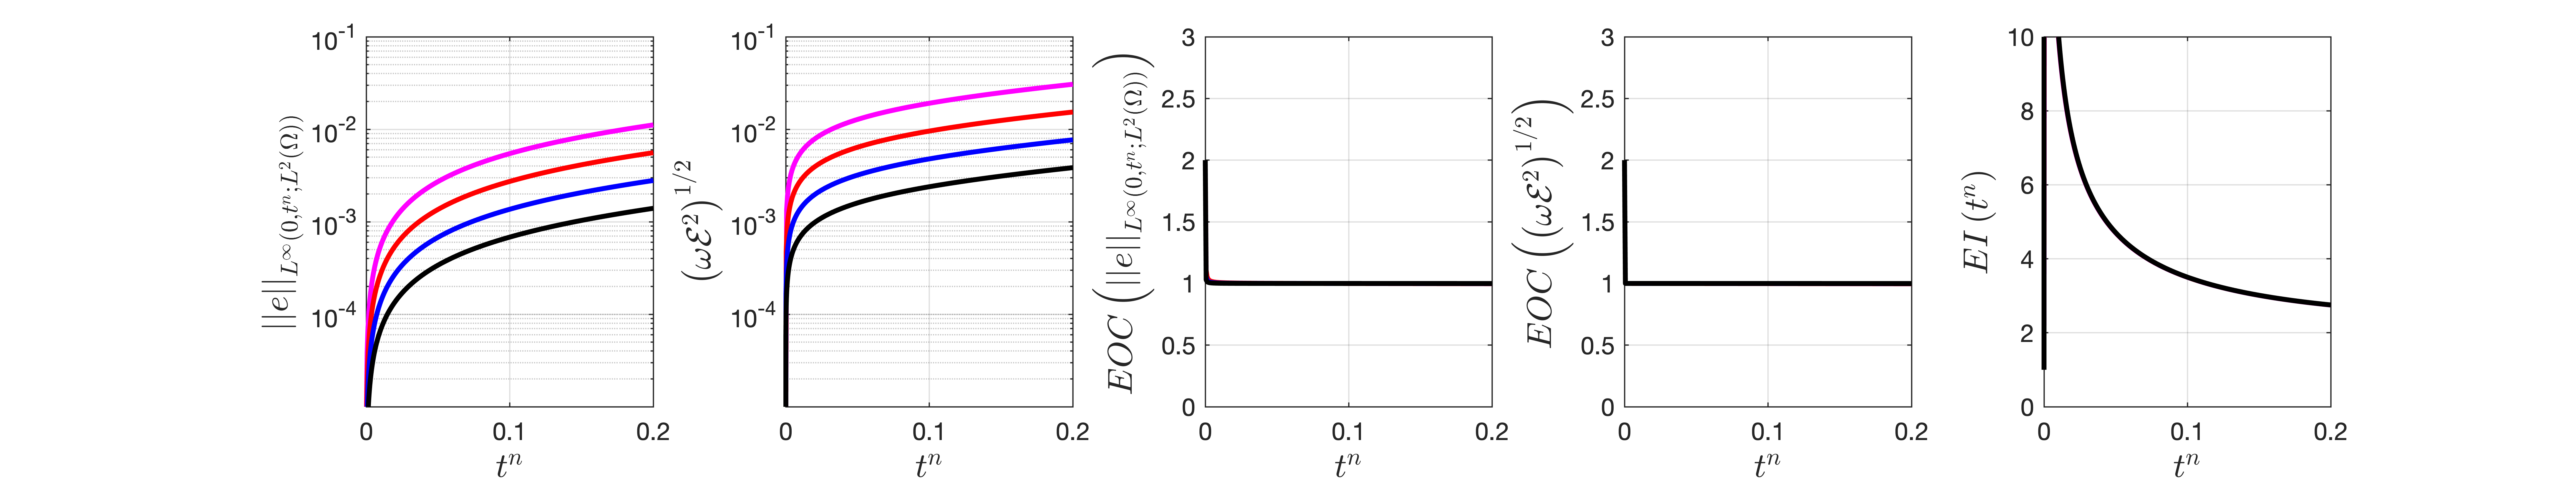
\includegraphics[width=\textwidth]{../figures/fig_LxF_preshockplots_1x5_sin_IC_P3_burgers}	
		\caption{
			\label{fig:Burgers_LxF_preshock}
		Pre-shock.
		}
	\end{subfigure}
	\\
	\begin{subfigure}[b]{\textwidth}
		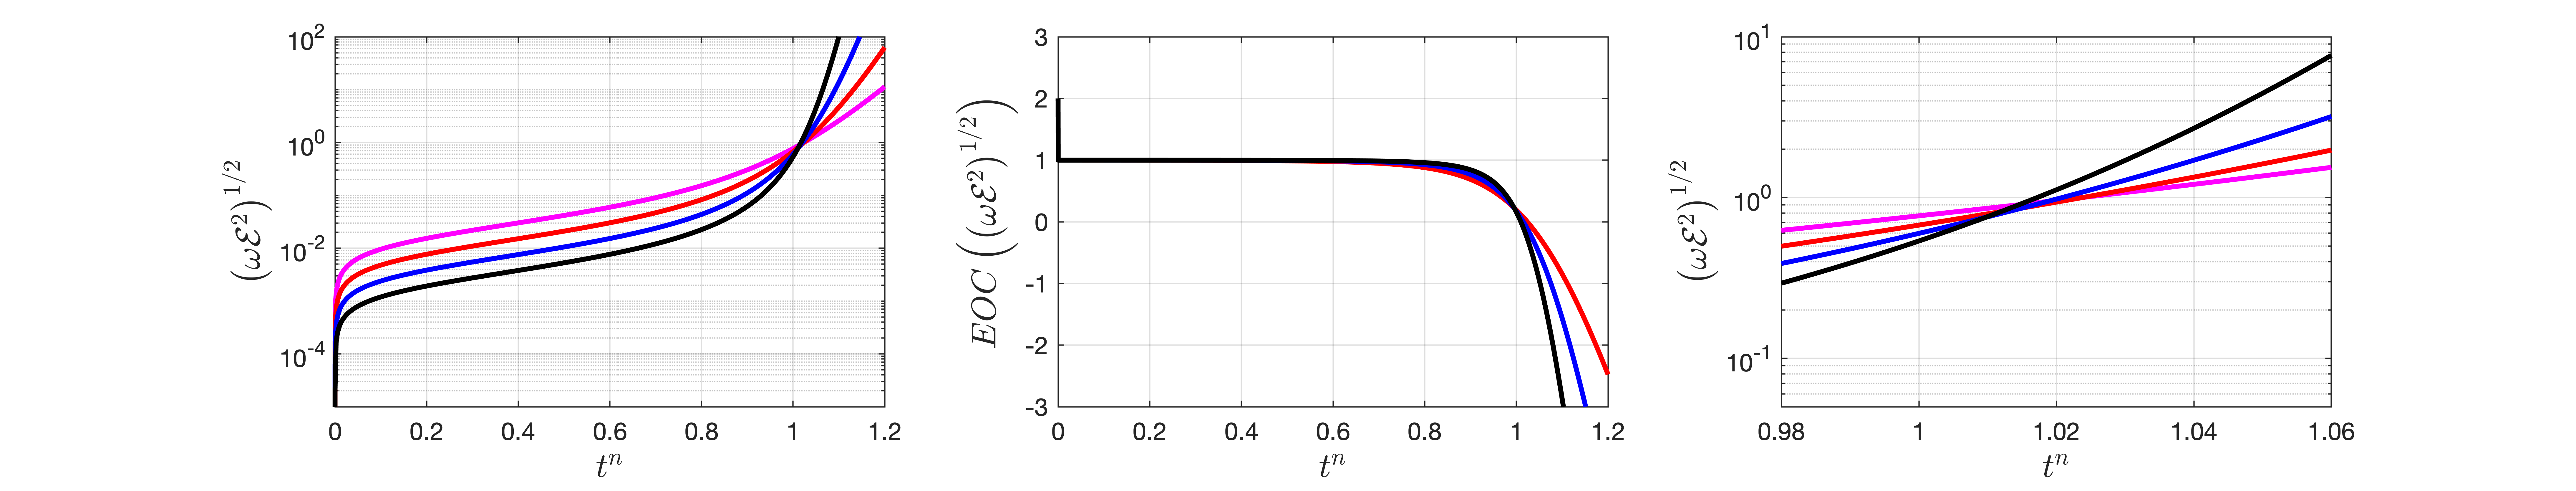
\includegraphics[width=\textwidth]{../figures/fig_LxF_postshockplots_1x5_sin_IC_P3_burgers}	
		\caption{\label{fig:Burgers_LxF_postshock}
		Post-shock.
		}
	\end{subfigure}
	\caption{\label{fig:LxF} Errors and asymptotic
		convergence rates for abound constructed using a bilinear interpolant for the Lax-Friedrichs scheme,
		(\ref{eq_F_LxF_cons}), for Burgers' equation with sinusoidal initial conditions and periodic boundary conditions given by (\ref{eq_burgers}).  The simulations were
		conducted over a family of meshes with discretisation parameter $h
		= 2^{-m}, m = 11,\dots 14$, with a timestep $\tau =
		\tfrac{h}{10}$. Note that the estimate is optimal prior to shock formation, and that it blows up once the shock forms,  as the exponential factor in (\ref{eq:burgers_bound}) blows up at $t\approx1$. }
\end{figure}
\begin{figure}[H]
	\begin{subfigure}[b]{\textwidth}
		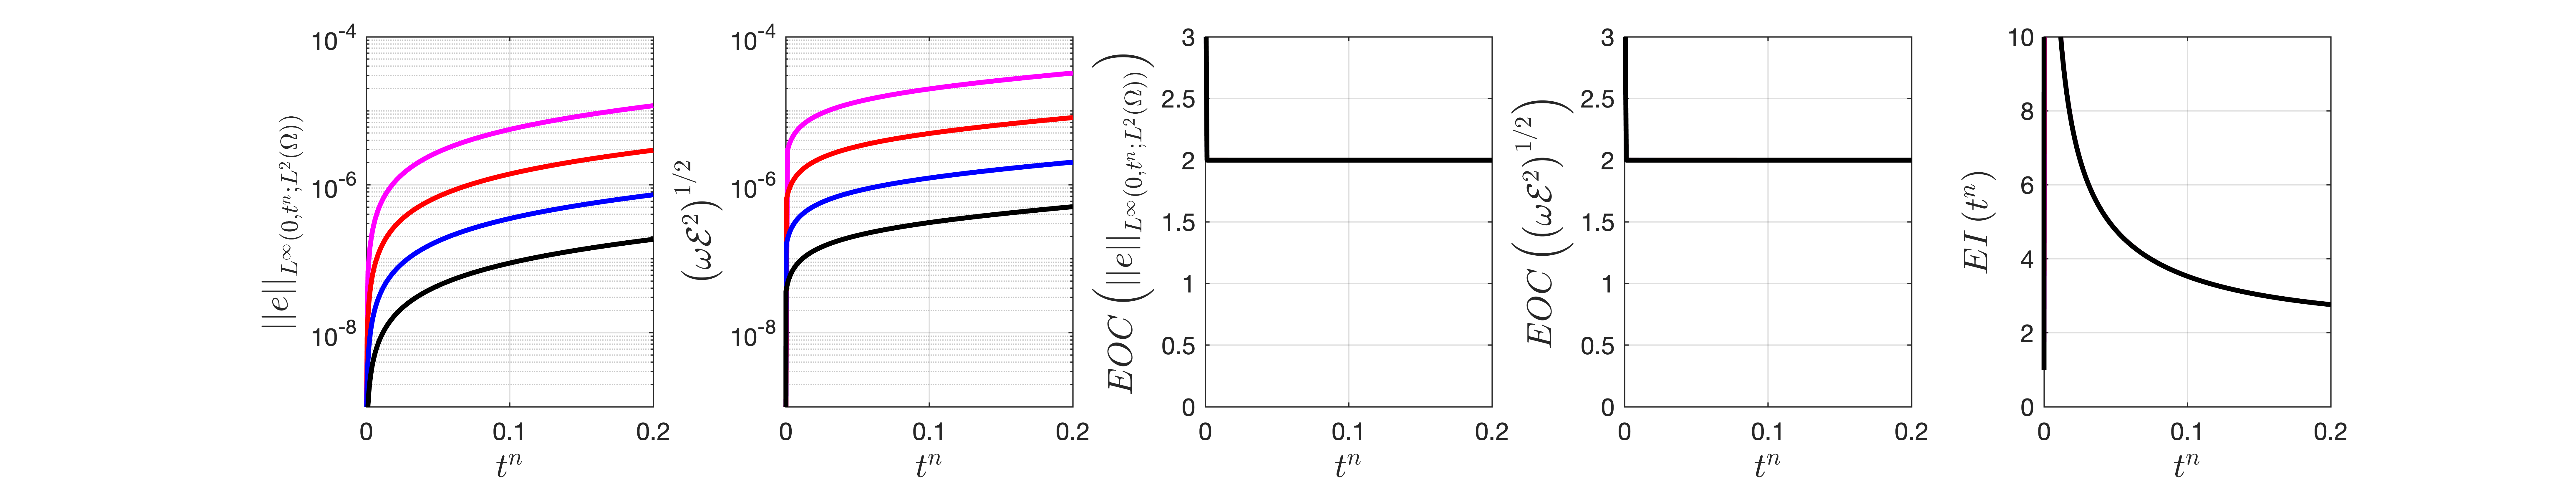
\includegraphics[width=\textwidth]{../figures/fig_LxW_preshockplots_1x5_sin_IC_P3_burgers}	
		\caption{
			\label{sfig:LxF_burgers_preshock}
			Pre-shock.
		}
	\end{subfigure}
	\\
	\begin{subfigure}[b]{\textwidth}
		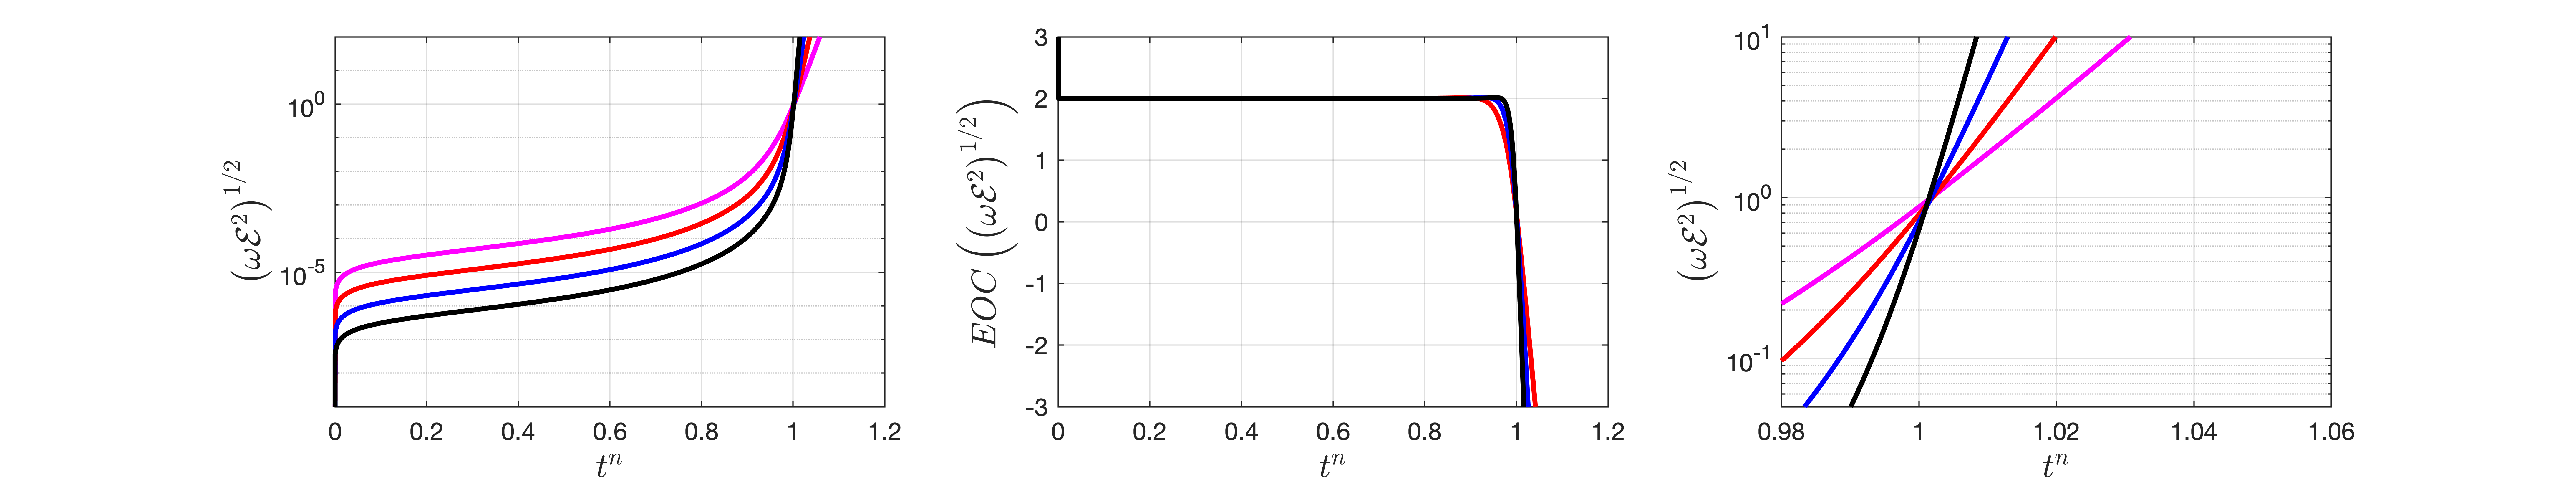
\includegraphics[width=\textwidth]{../figures/fig_LxW_postshockplots_1x5_sin_IC_P3_burgers}	
		\caption{\label{sfig:LxF_burgers_postshock}
		Post-shock.
		}
	\end{subfigure}
	\caption{\label{fig:LxW} Errors and asymptotic convergence
          rates for the Lax-Wendroff scheme, (\ref{eq_LxW_scheme}),
          for Burgers' equation with sinusoidal initial conditions and
          periodic boundary conditions given by
          (\ref{eq_burgers}). The simulations were conducted over a
          family of meshes with discretisation parameter $h = 2^{-m},
          m = 9,\dots 12$, with a timestep $\tau = \tfrac{h}{10}$. The a posteriori bound is constructed using a Hermite interpolant in time and a WENO3 interpolant in space.  The estimate is optimal prior to
          shock-formation.   In the
          post-shock regime the bound blows up, because the exponential factor in (\ref{eq:burgers_bound}) blows up at $t\approx1$.}
\end{figure}
\begin{figure}[H]
	\begin{subfigure}[b]{\textwidth}
		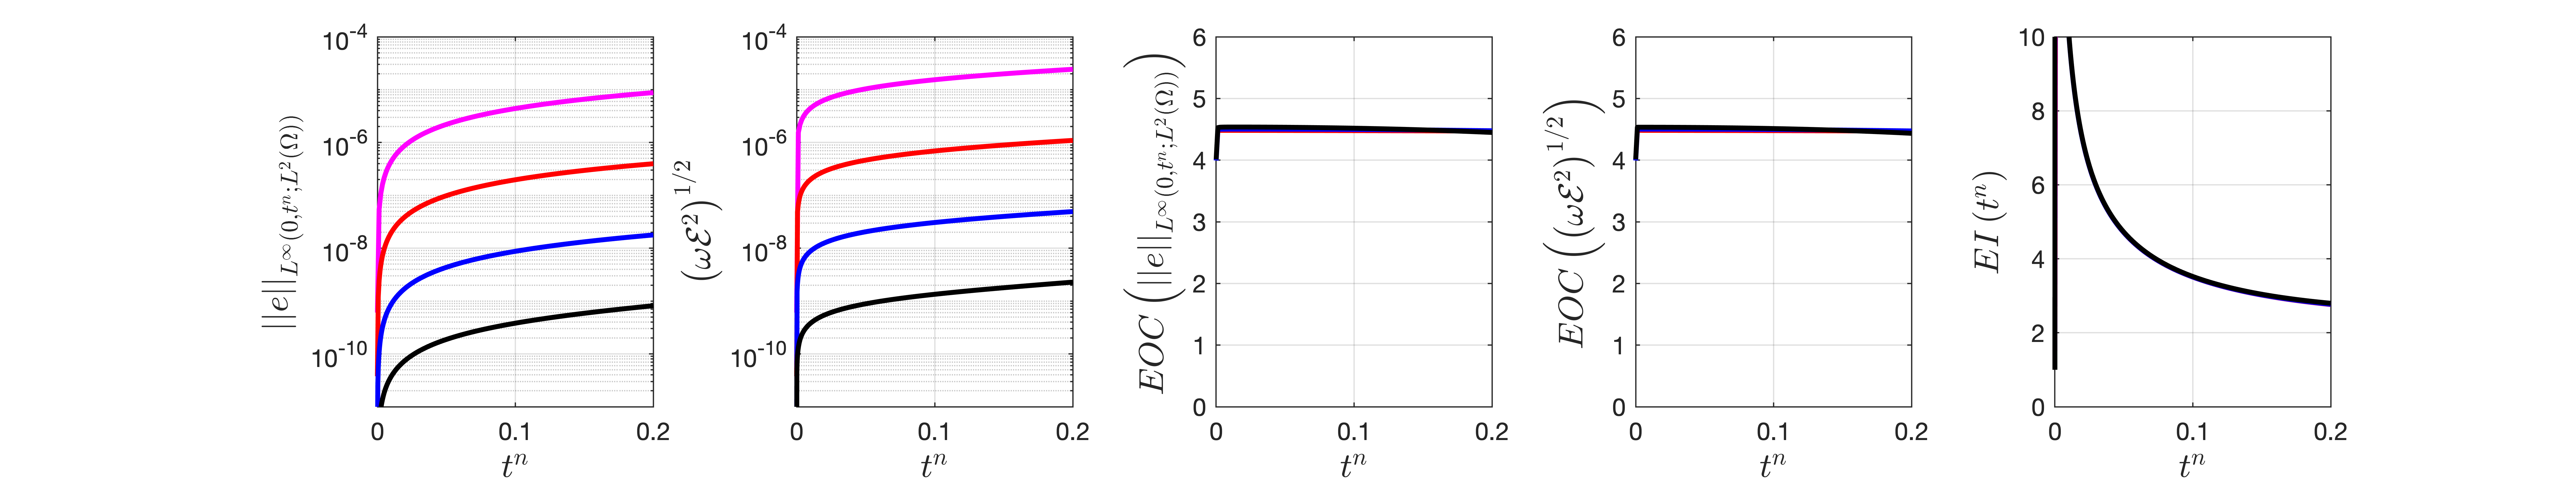
\includegraphics[width=\textwidth]{../figures/fig_SSP3WENO3_prehockplots_1x5_sin_IC_P3_burgers}	
		\caption{
			\label{fig:SSP3WENO3_burgers_P3_preshock}
			Pre-shock.
		}
	\end{subfigure}
	\\
	\begin{subfigure}[b]{\textwidth}
		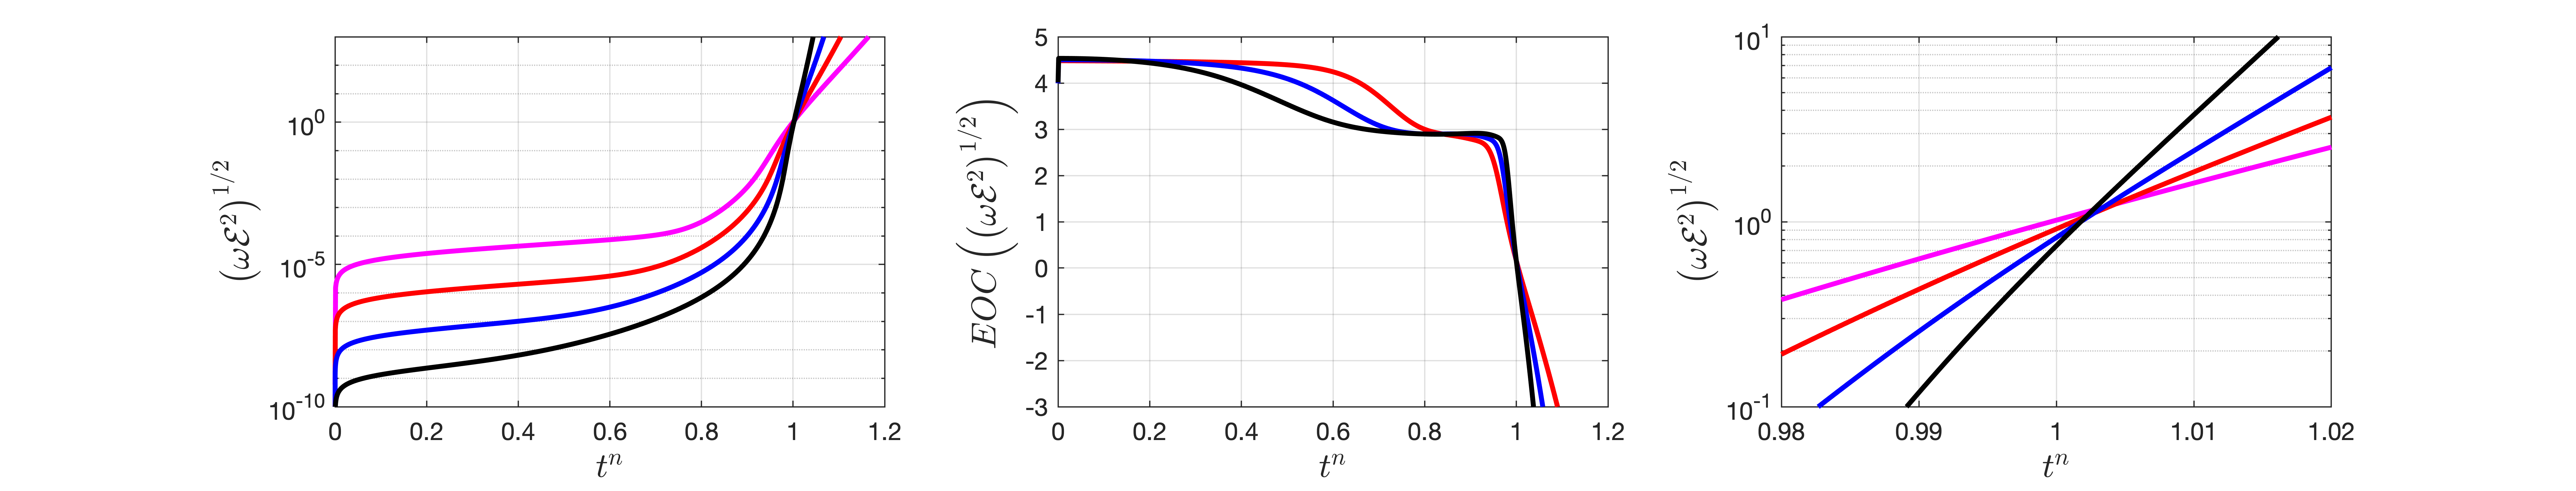
\includegraphics[width=\textwidth]{../figures/fig_SSP3WENO3_postshockplots_1x5_sin_IC_P3_burgers}	
		\caption{\label{fig:SSP3WENO3_burgers_P3_postshock}
			Post-shock. 
		}
	\end{subfigure}
	\caption{\label{fig:SSP3WENO_burgers} Errors and asymptotic
          convergence rates for the SSP3-WENO3 discretisation of Burgers' equation with a
          sinusoidal initial condition and periodic boundary
          conditions (\ref{eq_burgers}).  The reconstruction is obtained using  a Hermite temporal interpolant and a WENO3 spatial interpolant.  The simulations were
          conducted over a family of meshes with discretisation
          parameter $h = 2^{-m}, \,m = 9,\dots 12$, with a timestep
          $\tau = \tfrac{h}{10}$.  Notice that  the estimator loses optimality gradually in the interval $0.2\leq t \leq 0.8$.  This is because the solution itself is losing regularity, only this time the scheme and the residual are both of sufficiently high order  to capture this.  At $t\approx 1$ the shock forms and the exponential factor in (\ref{eq:burgers_bound})  blows up.}
\end{figure}
In order to explain the behaviour of the bound (\ref{eq:burgers_bound}), we decouple  the time-accumulation factor from the residual component of the post-processor (see Fig. \ref{fig:SSP3WENO_burgers_decoupled}).  Notice that at $ t\approx1$ the exponential factor blows up rapidly as $v_x$ blows up.  The reason for this is that at $t=1$ the solution starts forming a shock.  This explains the behaviour for $t>=1$.  
\begin{figure}[H]	
		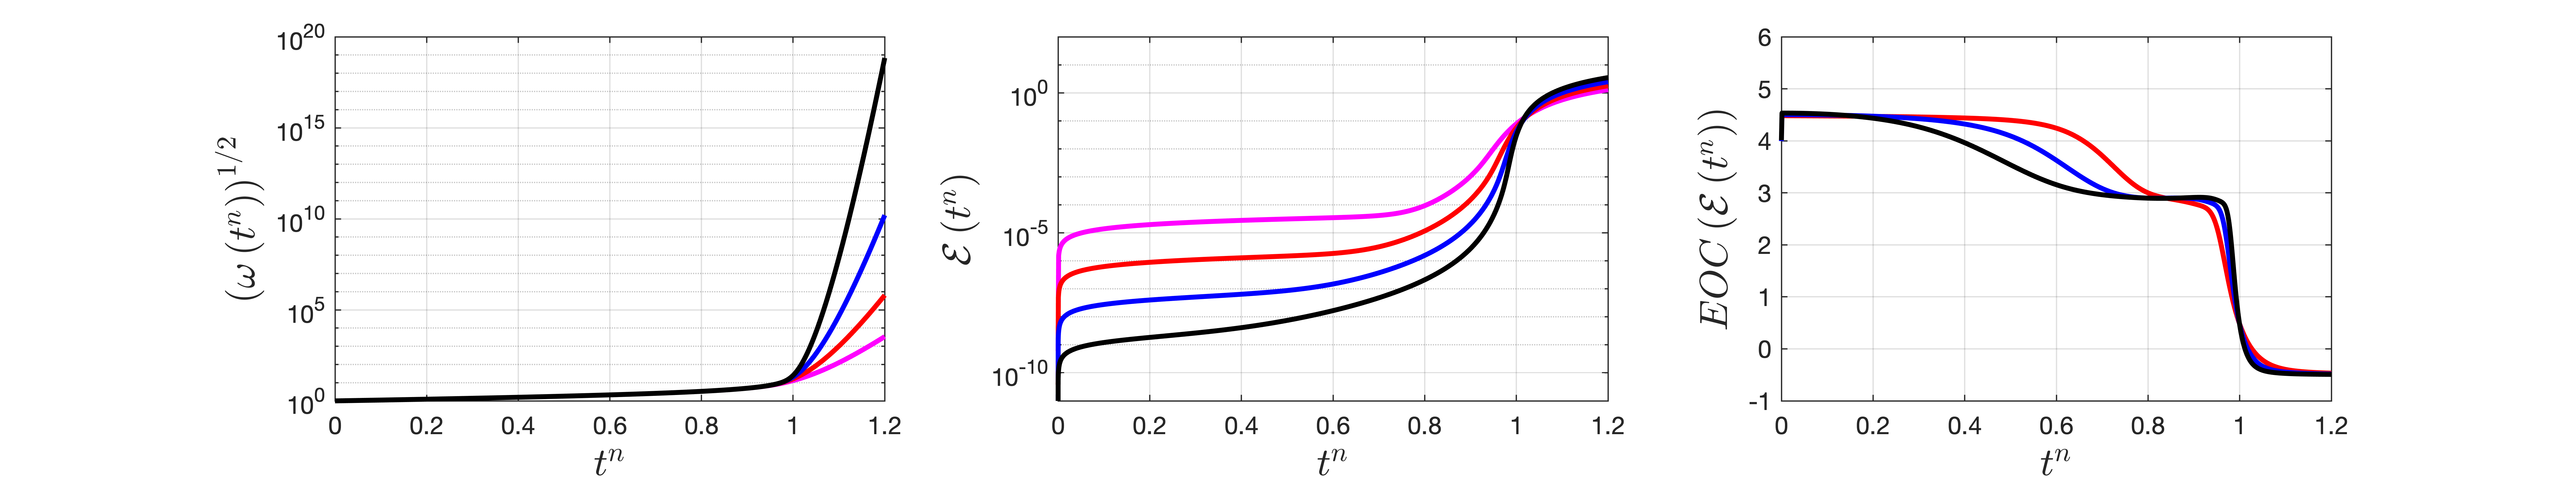
\includegraphics[width=\textwidth]{../figures/fig_SSP3WENO3_postshockplots_1x5_sin_IC_burgers_decoupled}	
	\caption{\label{fig:SSP3WENO_burgers_decoupled}  Decoupling for the post-processor the cubic spatio-temporal  interpolant of SSP3-WENO3
		approximations of Burgers' equation with a sinusoidal initial condition and periodic boundary conditions
		(\ref{eq_burgers}).  The simulations were conducted over a family of
		meshes with discretisation parameter $h = 2^{-m}, m = 9,\dots 12$,
		with a timestep $\tau = \tfrac{h}{10}$. The blow-up in the time accumulation term is because of the spatial derivative in the exponential factor, which becomes exceedingly large in the presence of shocks. }
\end{figure}

\subsection{Test 2:  Shallow Water equation.  }  We benchmark the behaviour of the residual for the shallow water equations.
\begin{figure}[H]	
	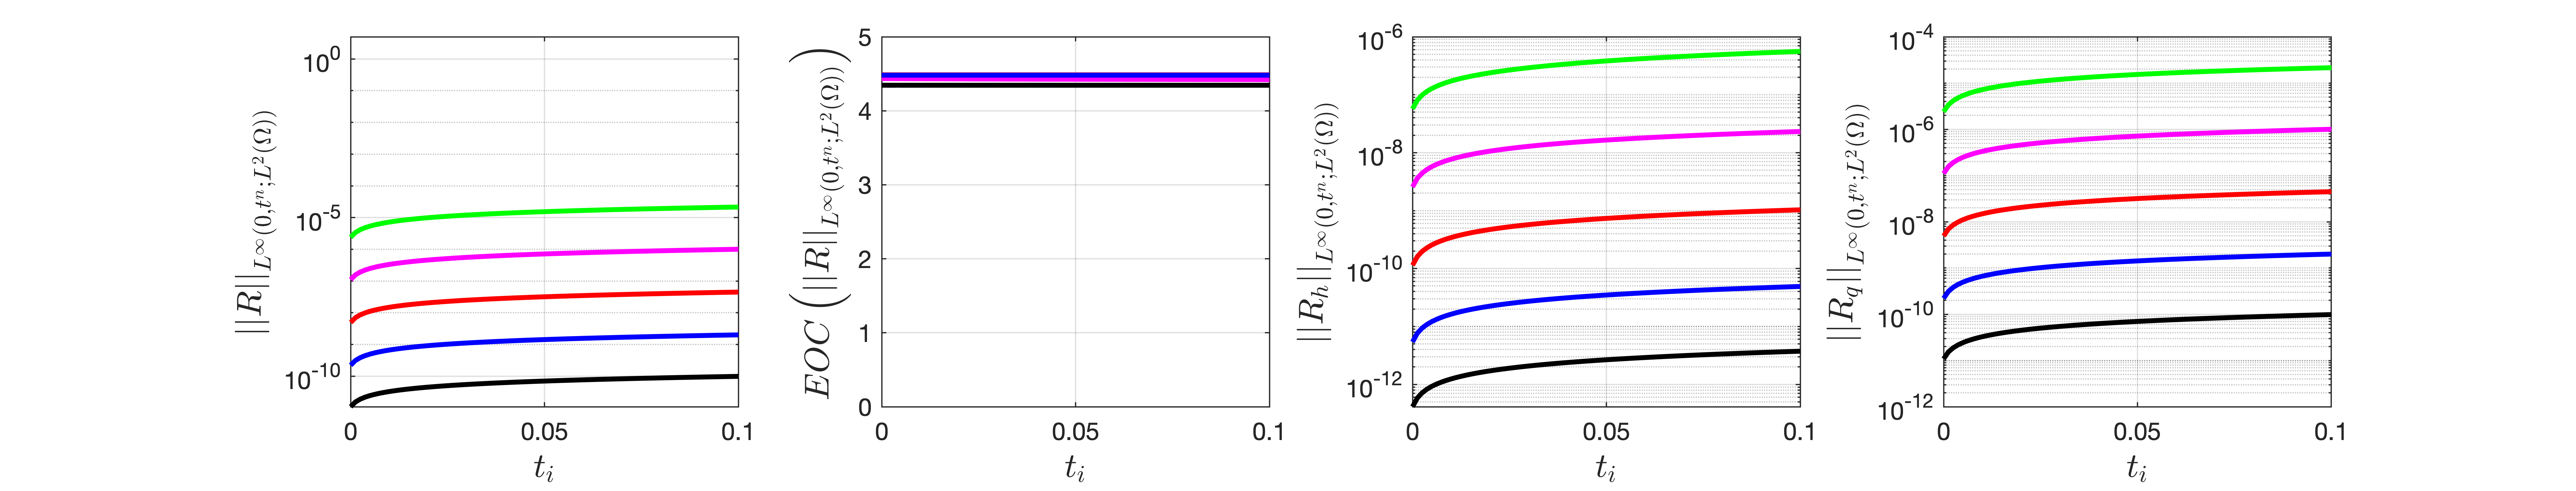
\includegraphics[width=\textwidth]{../figures/fig_SHW_RK3_WENO3_rec3_fixed_gsplots_1x5_sin_IC_P3_shw}	
	\caption{\label{fig:SSP3WENO_SHW} Bench marking for the shallow-water equations with a sinusoidal initial condition and periodic boundary conditions. We use an SSP3-WENO3 scheme with $h = 2^{-m}, m = 9,\dots 12$,
		with a timestep $\tau = \tfrac{h}{10}$.  The bound is constructed using a Hermite-WENO-3 interpolant.  Observe that the residual maintains a high order of convergence throughout the simulation.}
\end{figure}

The last test in this section is presented in order to motivate adaptivity in the context of finite difference schemes for conservation laws. We highlight additional challenges that arise in implementing adaptivity, even for scalar examples in one spatial dimension.  
\subsection{Test 3: Parasite detection in 1D} \label{subsec:parasite}In this test we investigate the resulting behaviour of (\ref{eq_prelim_bound}) in the presence of parasitic waves and we verify the capability of the bound we construct using Defns \ref{defn_temp_rec} and \ref{defn_spatio-temporal reconstruction} to detect such waves. Very briefly, parasitic waves are numerical artefacts which are generated whenever the numerical solution encounters some discontinuity in the numerical model. Such discontinuities include local changes in grid spacing (see \cite{vichnevetsky1981propagation}),  abrupt changes in some aspect of the specific PDE model, such as a discontinuous change in coefficients (see \cite{trefethen1982group}) or even a change in the PDE used in different regions of the domain, e.g. advection in one region and advection-diffusion in another, (see the work of \cite{giesselmann2017posteriori} for more details on model adaptivity).  

We use a Crank-Nicholson in time  Central-Space scheme  on a piecewise non-uniform grid given by
\begin{equation}\label{eq_grid_spacing_piecewise_nonu}
h_j=x_{j+1}-x_j= \begin{cases}
2^{-\qp{9}} \quad&\text{if}\quad x_{j+1}>L/2,\\
2^{-\qp{10}}\quad&\text{otherwise}
\end{cases}.
\end{equation}


\begin{Rem}[Truncation error of the central difference quotient]\label{rem_central_truncation}
	The truncation error of the usual central difference quotient,
	\begin{equation}\label{eq_normal_quotient}
	u_x\approx \frac{U^n_{j+1}-U^n_{j-1}}{h_{j+1}+h_{j}},
	\end{equation}
	on a uniform grid is two globally. On a non-uniform grid, it is locally one wherever $\llbracket h_j\rrbracket:= h_{j+1}-h_{j}\neq 0$.  In order to ensure that the spatial discretisation is second order on a non-uniform grid, we use the modified  quotient 
	\begin{equation}\label{eq_modified_quotient}
	u_x \approx \qp{\frac{1}{h_{j+1}} - \frac{1}{h_j+h_{j+1} } }U^n_{j+1} + 
	\qp{\frac{1}{h_{j}} - \frac{1}{h_{j+1} } }U^n_{j} +
	\qp{\frac{1}{h_j+h_{j+1} } -\frac{1}{h_{j}} }U^n_{j-1},
	\end{equation}
	which is order two globally  on a non-uniform grid as well and simplifies to (\ref{eq_normal_quotient}) on a uniform grid. 
\end{Rem}
In order to demonstrate the effect of the parasite, we plot $\Norm{R}_{\leb{2}\qp{I_j}}$, for $R$ given by  (\ref{eq_reconstruction_gen_cons}) for  an exponential initial condition, 
\begin{equation}\label{eq_ic_parasites}
u_0\qp{x}=\exp\qp{-100\qp{x-0.25}^2},
\end{equation}
which makes the parasites more visible.  The results are shown in Fig. \ref{fig:CNCS_parasite}.

\/*
\begin{figure}[H]
	\centering
	\centering
	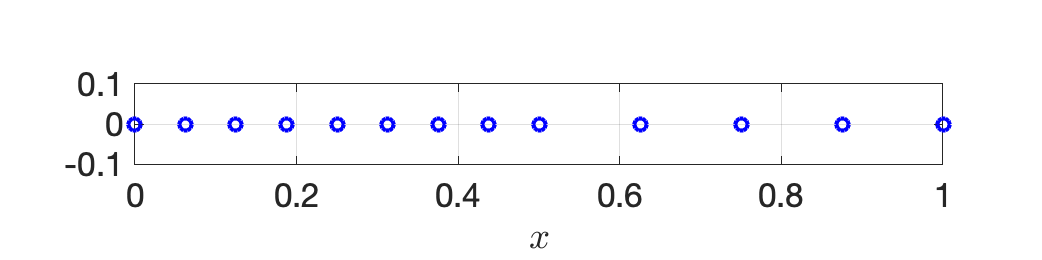
\includegraphics[scale=.5]{../figures/fig_grid_piecewise_nonu_2}	
	\caption{Piece-wise nonuniform grid.}
	\label{fig_grid_piecewise_nonu}
\end{figure}
*/

\begin{figure}[H]
	\centering
	\begin{subfigure}[b]{.3\textwidth}
		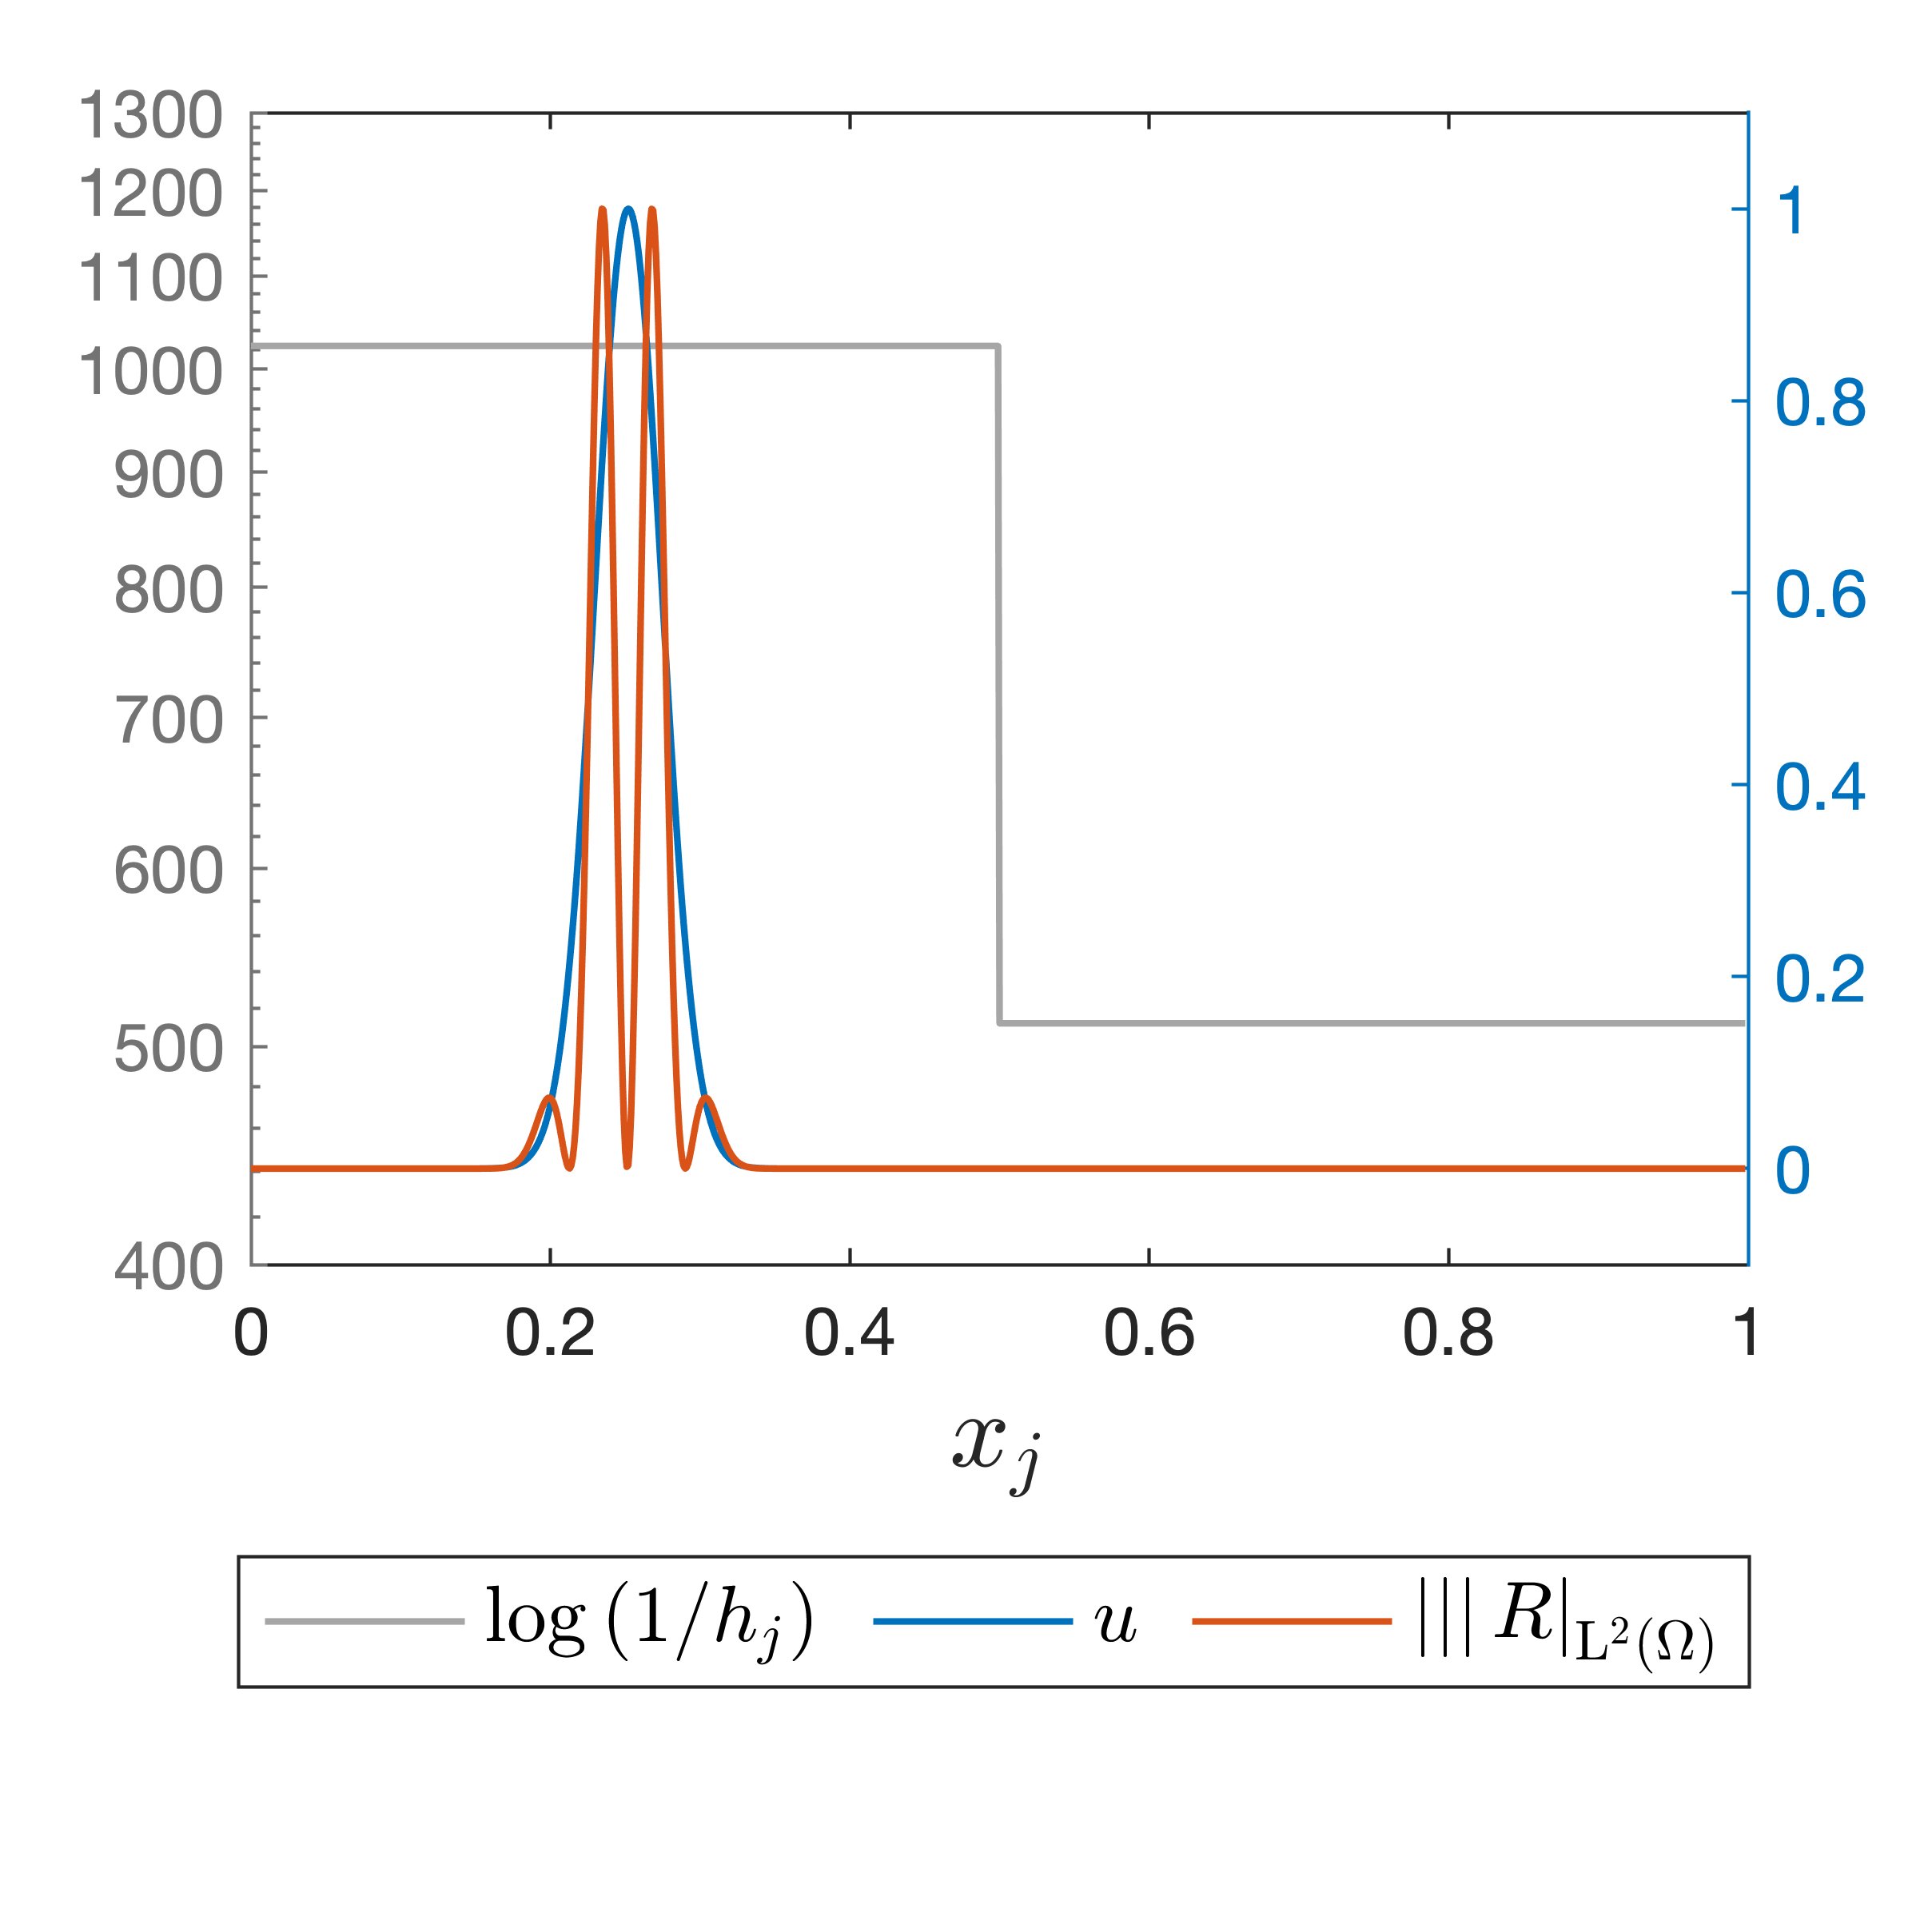
\includegraphics[width=\textwidth]{../figures/fig_CNCS_parasite_rep_20_zoom_off}	
		\caption{
			\label{fig:CNCS_parasite_1D_1}
			Before parasite forms.
		}
	\end{subfigure}
	\begin{subfigure}[b]{.3\textwidth}
		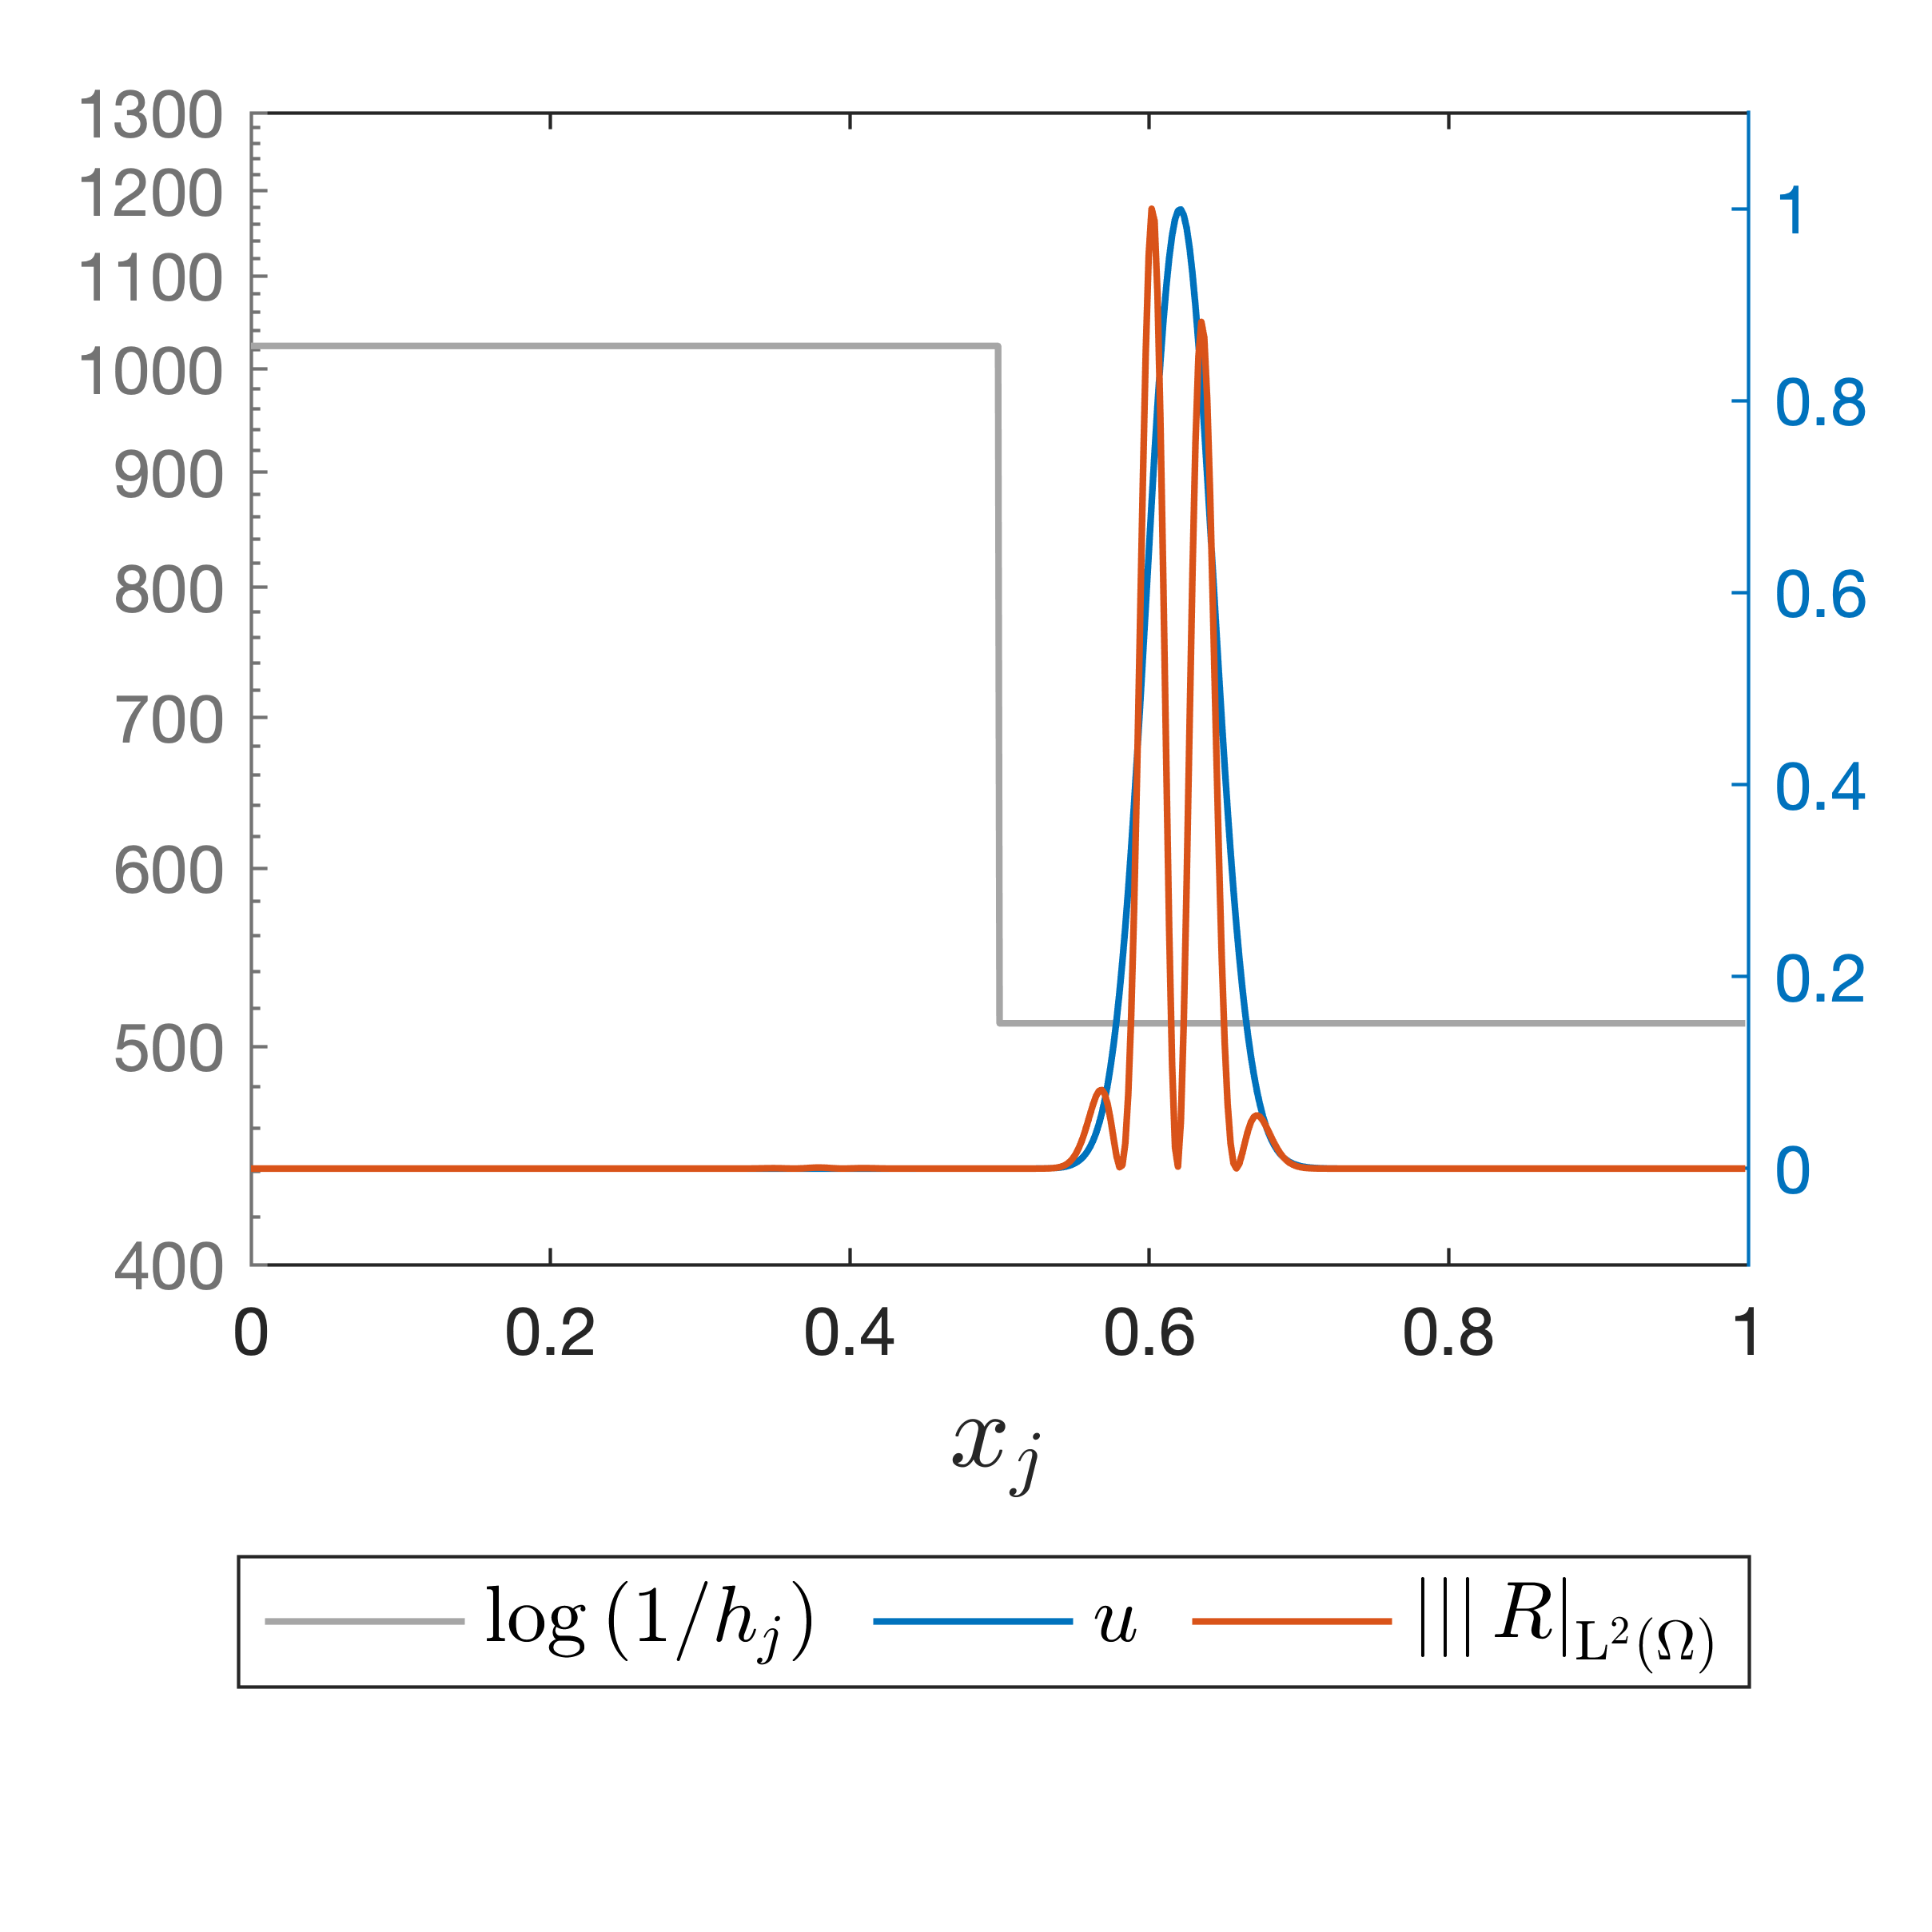
\includegraphics[width=\textwidth]{../figures/fig_CNCS_parasite_rep_3800zoom_off}	
		\caption{\label{fig:CNCS_parasite_1D_1}
			After parasite forms.
		}
	\end{subfigure}
	\begin{subfigure}[b]{.3\textwidth}
		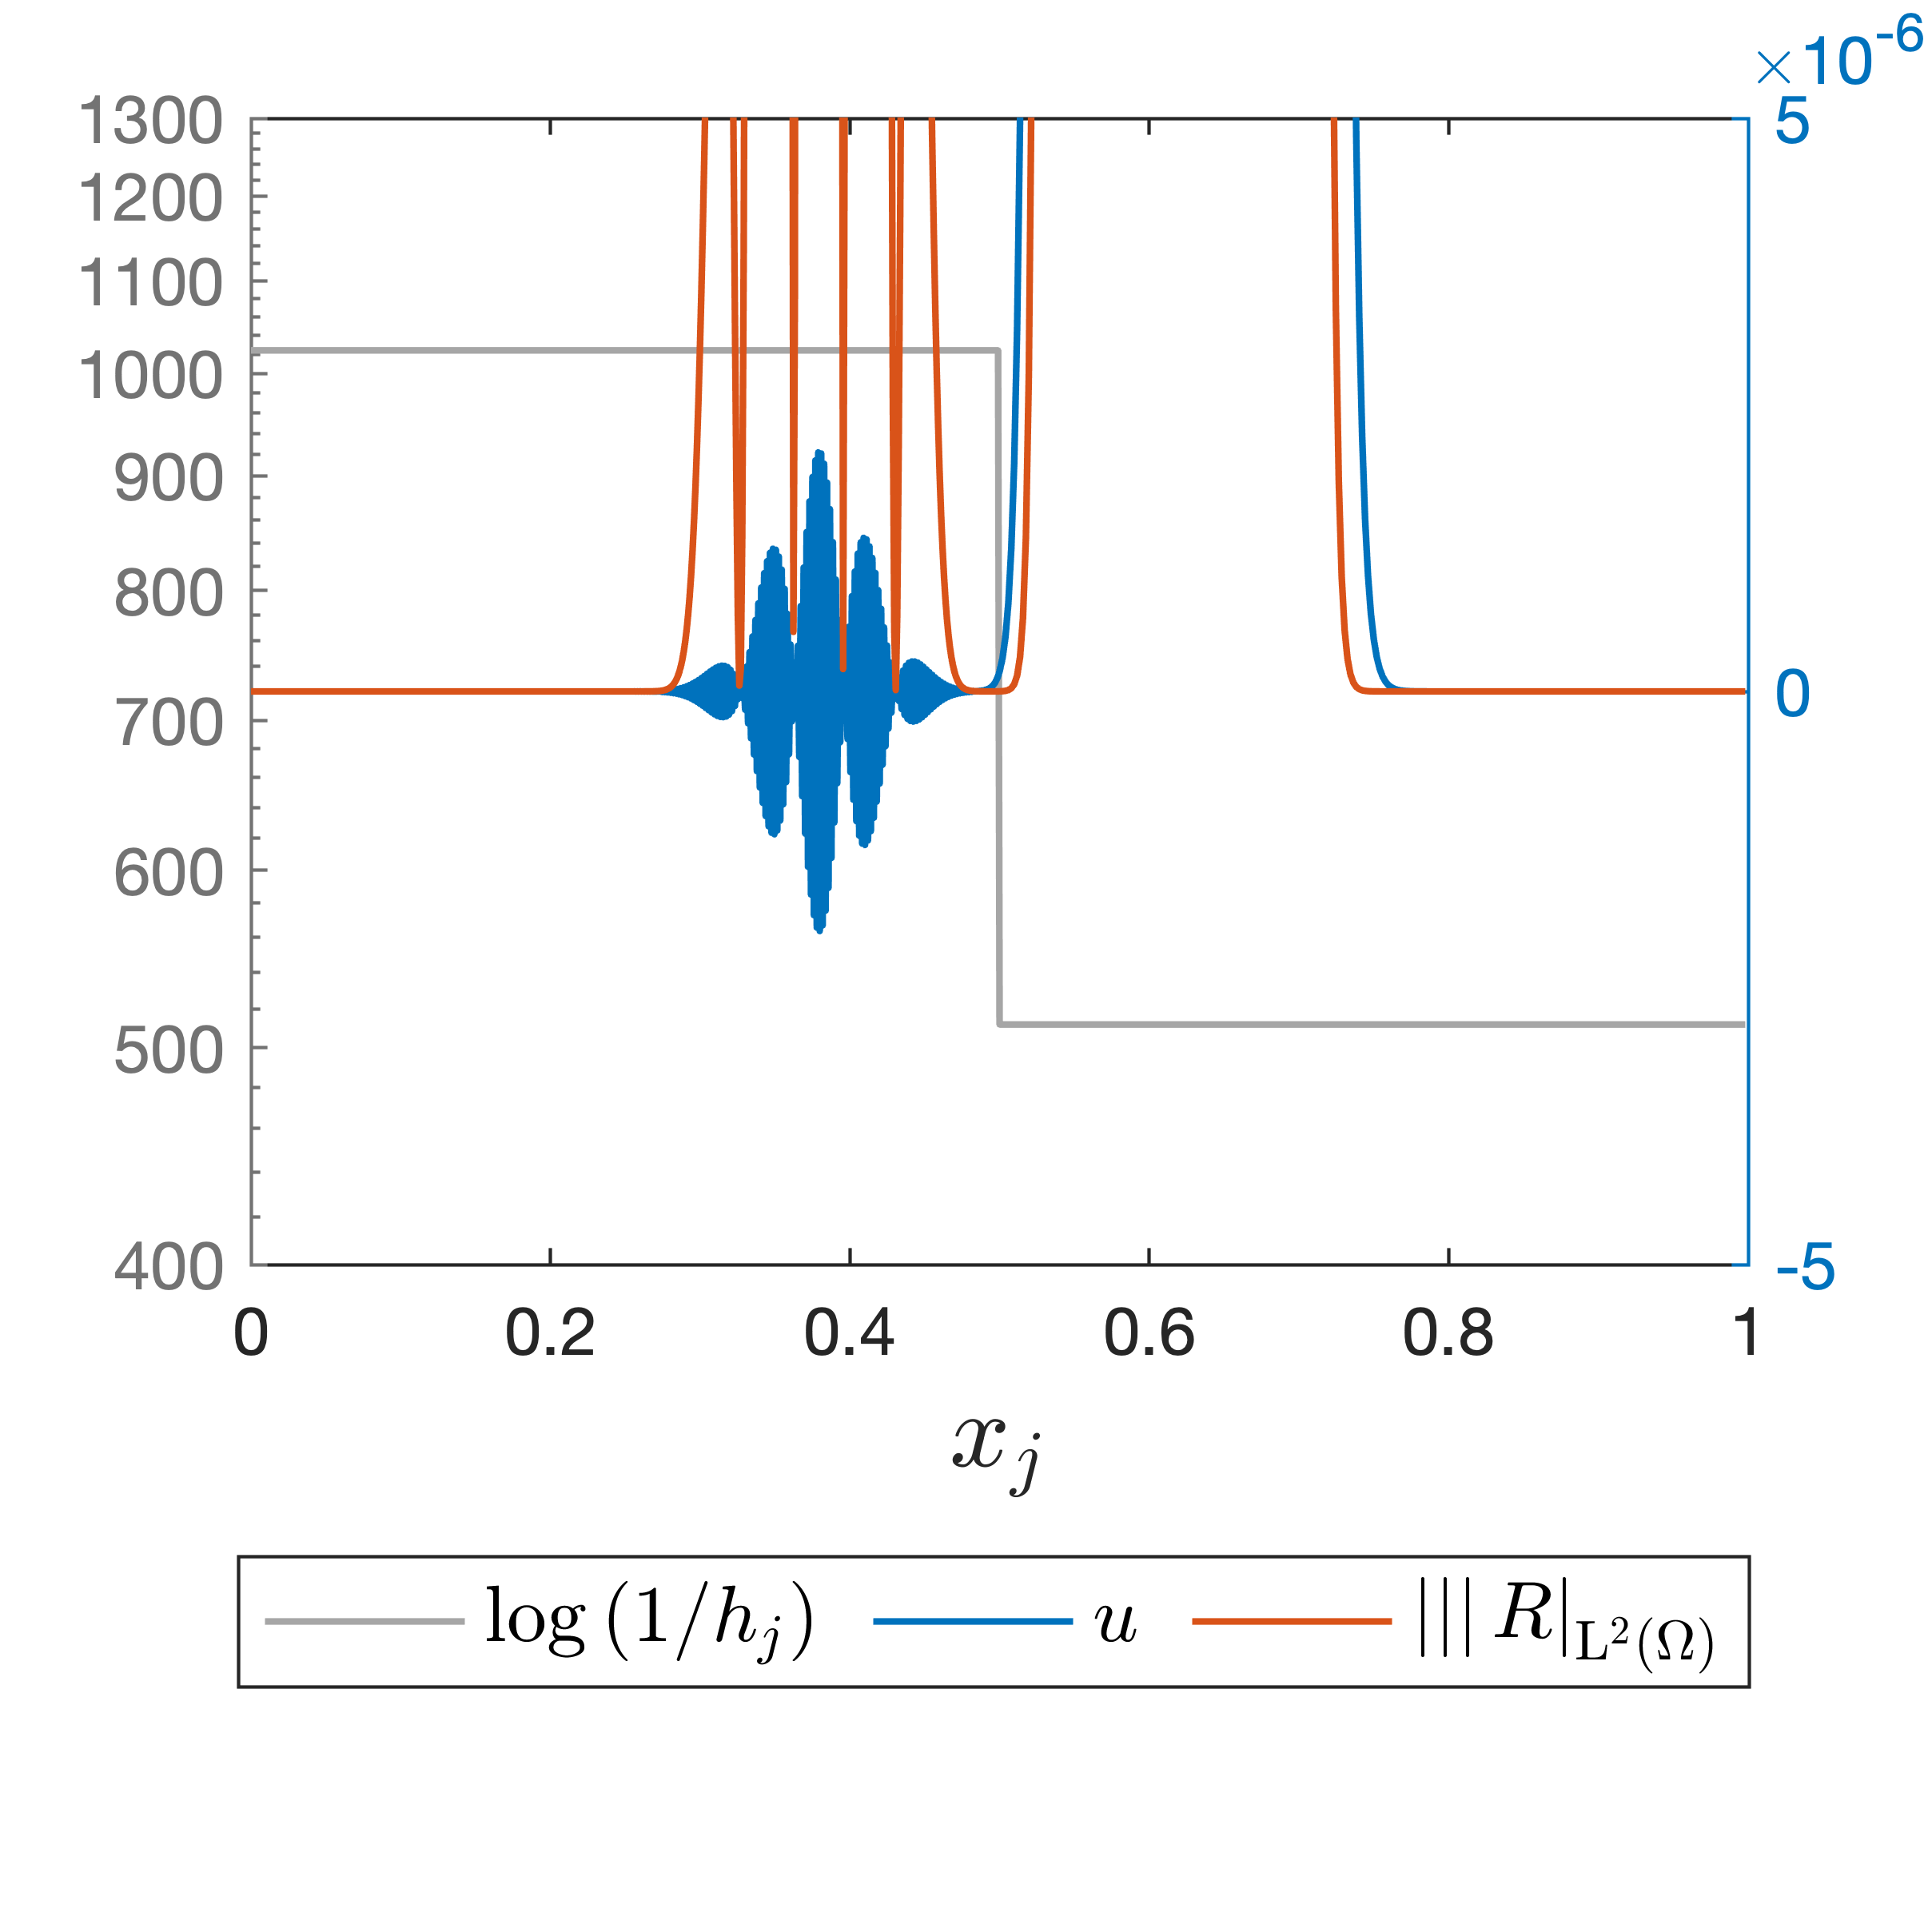
\includegraphics[width=\textwidth]{../figures/fig_CNCS_parasite_rep_3800zoom_on}	
		\caption{\label{fig:CNCS_parasite_1D_2_zoom}
			Magnified Parasite.
		}
	\end{subfigure}
\caption{A parasitic wave which occurs to due an abrupt mesh change.  We use a CNCS scheme on a grid given by (\ref{eq_grid_spacing_piecewise_nonu}) and a temporal-to-spatial step coupling of $\tau=\frac{h}{10}$.  We plot the solution and the normalized $\leb{2}$-norm of the local residual (\ref{eq_reconstruction_gen_cons}) before and after parasite formation.  The parasitic wave is the highly oscillatory wave in the right-most plot, which is zoomed in.  Notice that it is moving in the opposite direction from the solution. Such parasites can arise when implementing adaptivity and can rapidly pollute the computation. Notice that the residual detects and tracks the parasite.}
\label{fig:CNCS_parasite}
\end{figure}

%begin{figure}[H]
%	\begin{subfigure}[b]{.3\textwidth}
%		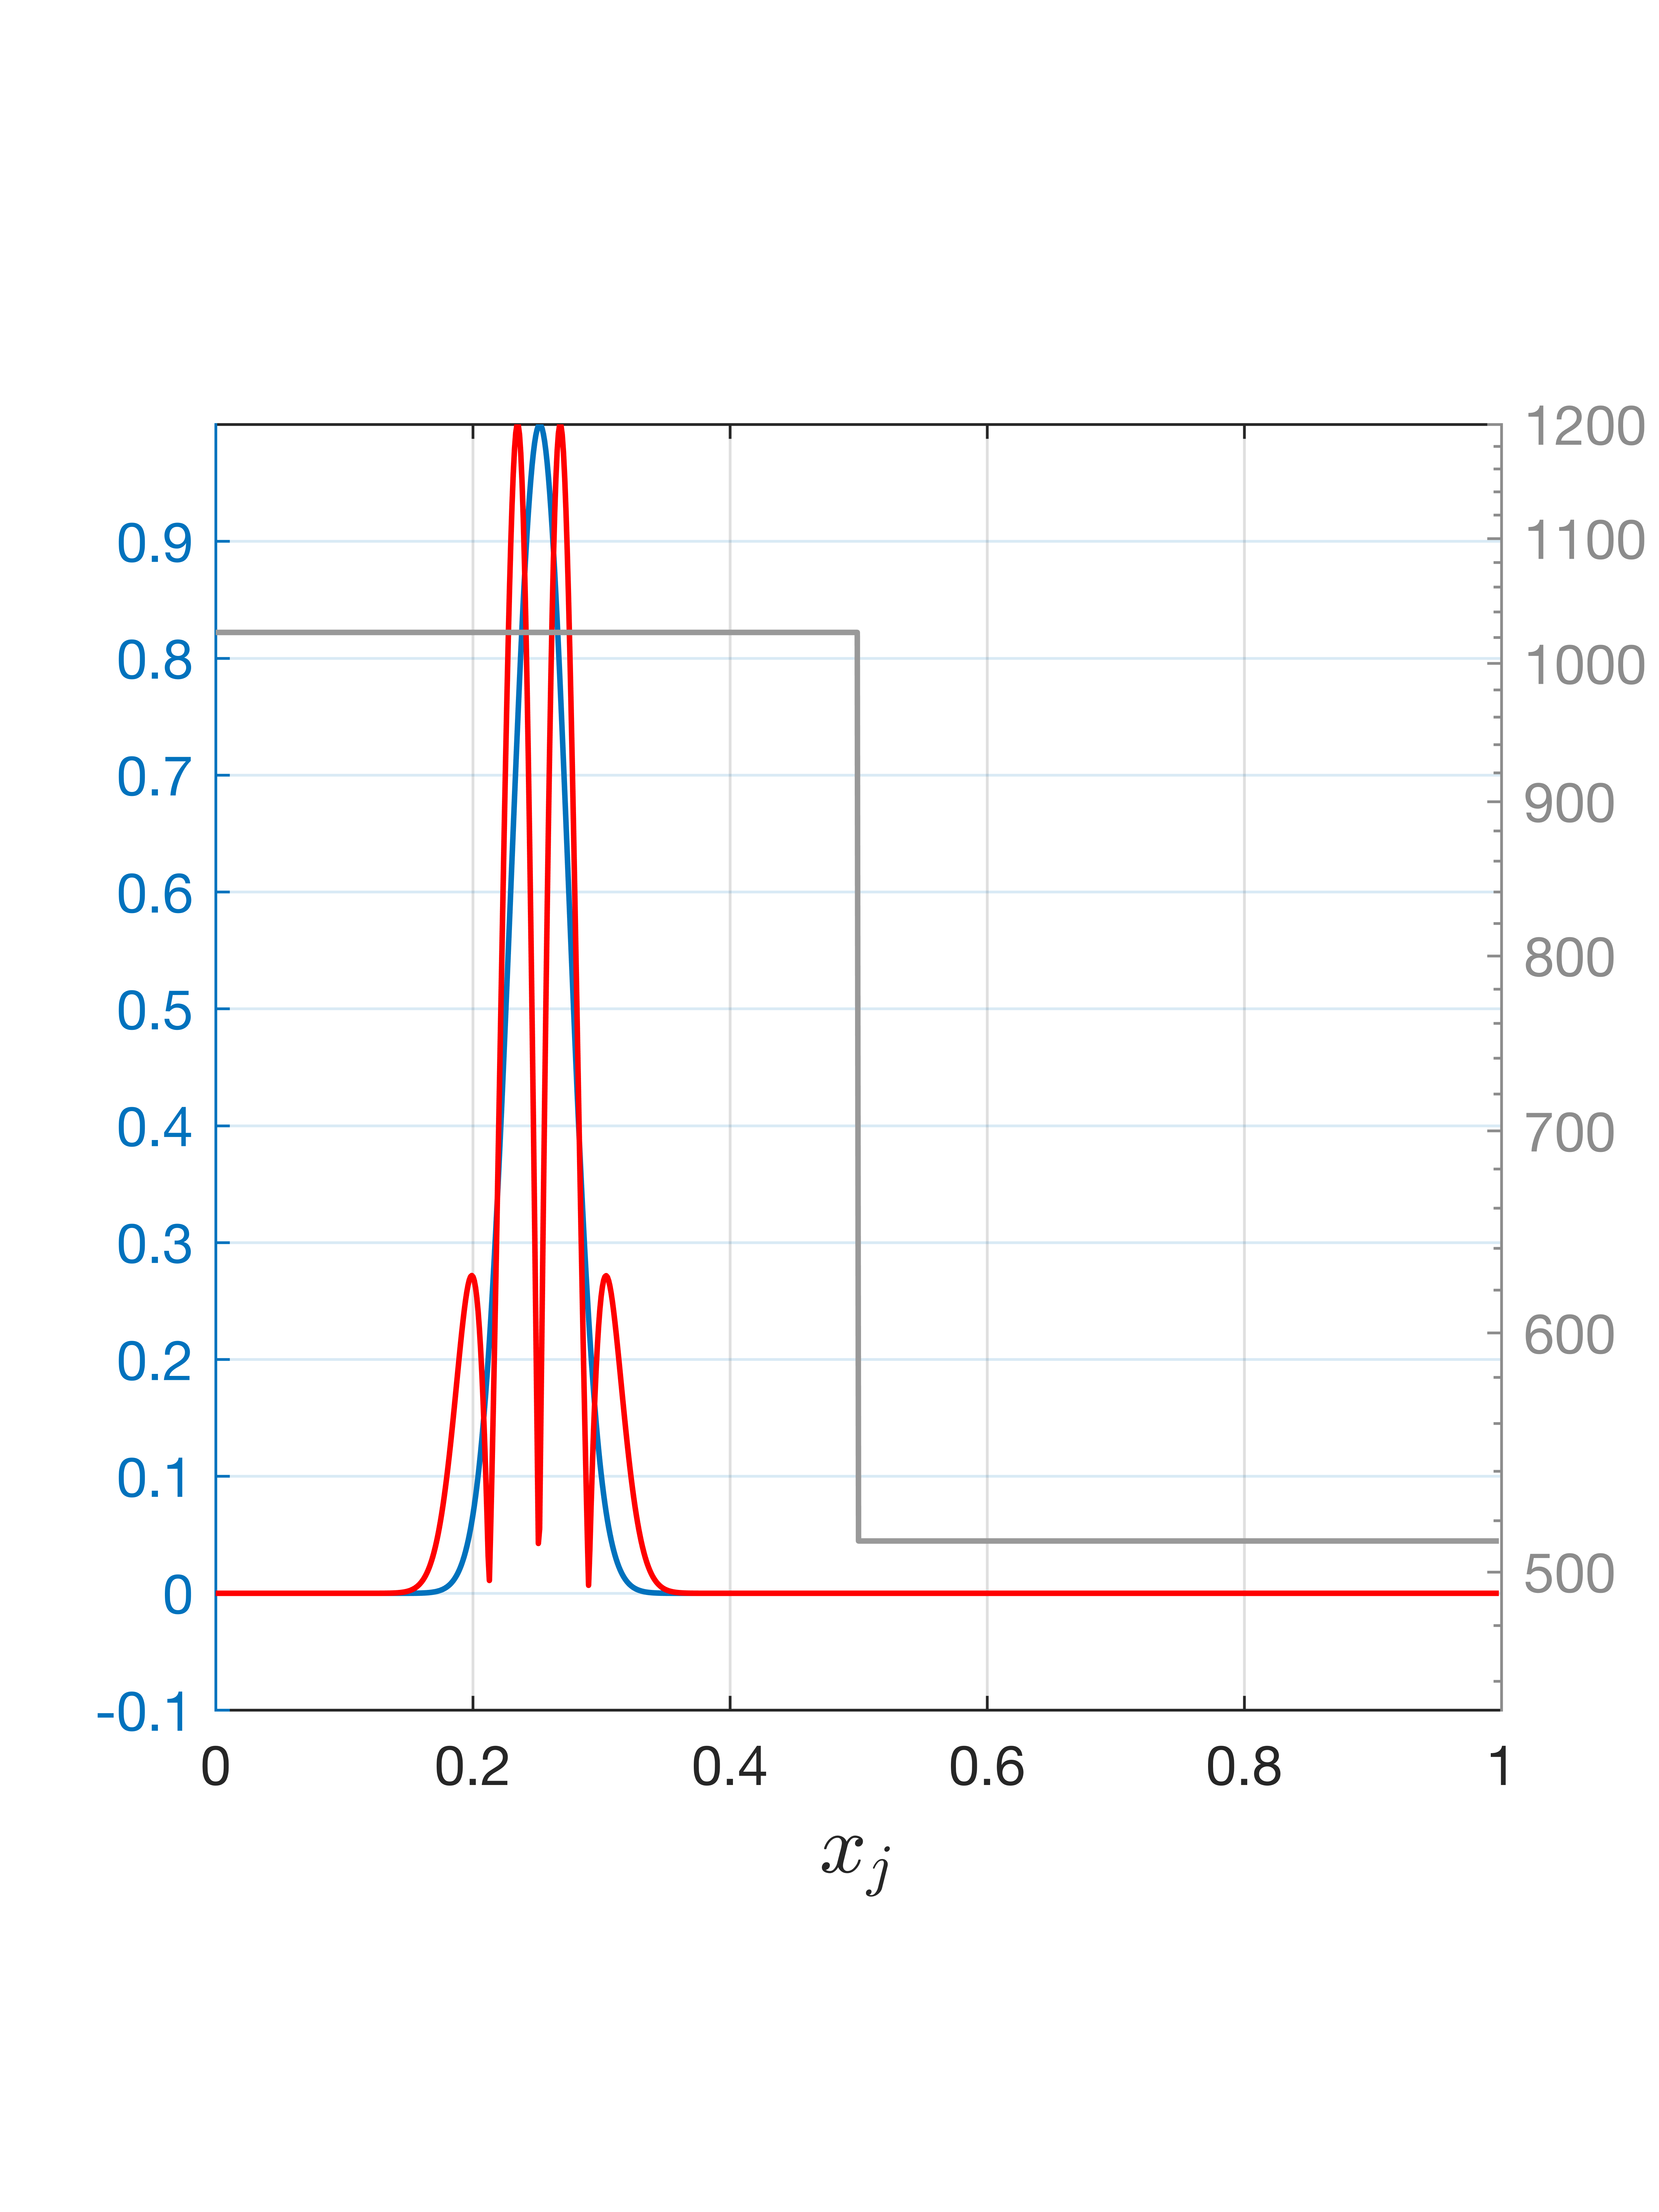
\includegraphics[width=\textwidth]{../figures/fig_CNCS_20_para_1}	
%		\caption{
			
%			Before parasite formation.
%		}
%	\end{subfigure}%
%	\begin{subfigure}[b]{.3\textwidth}
%		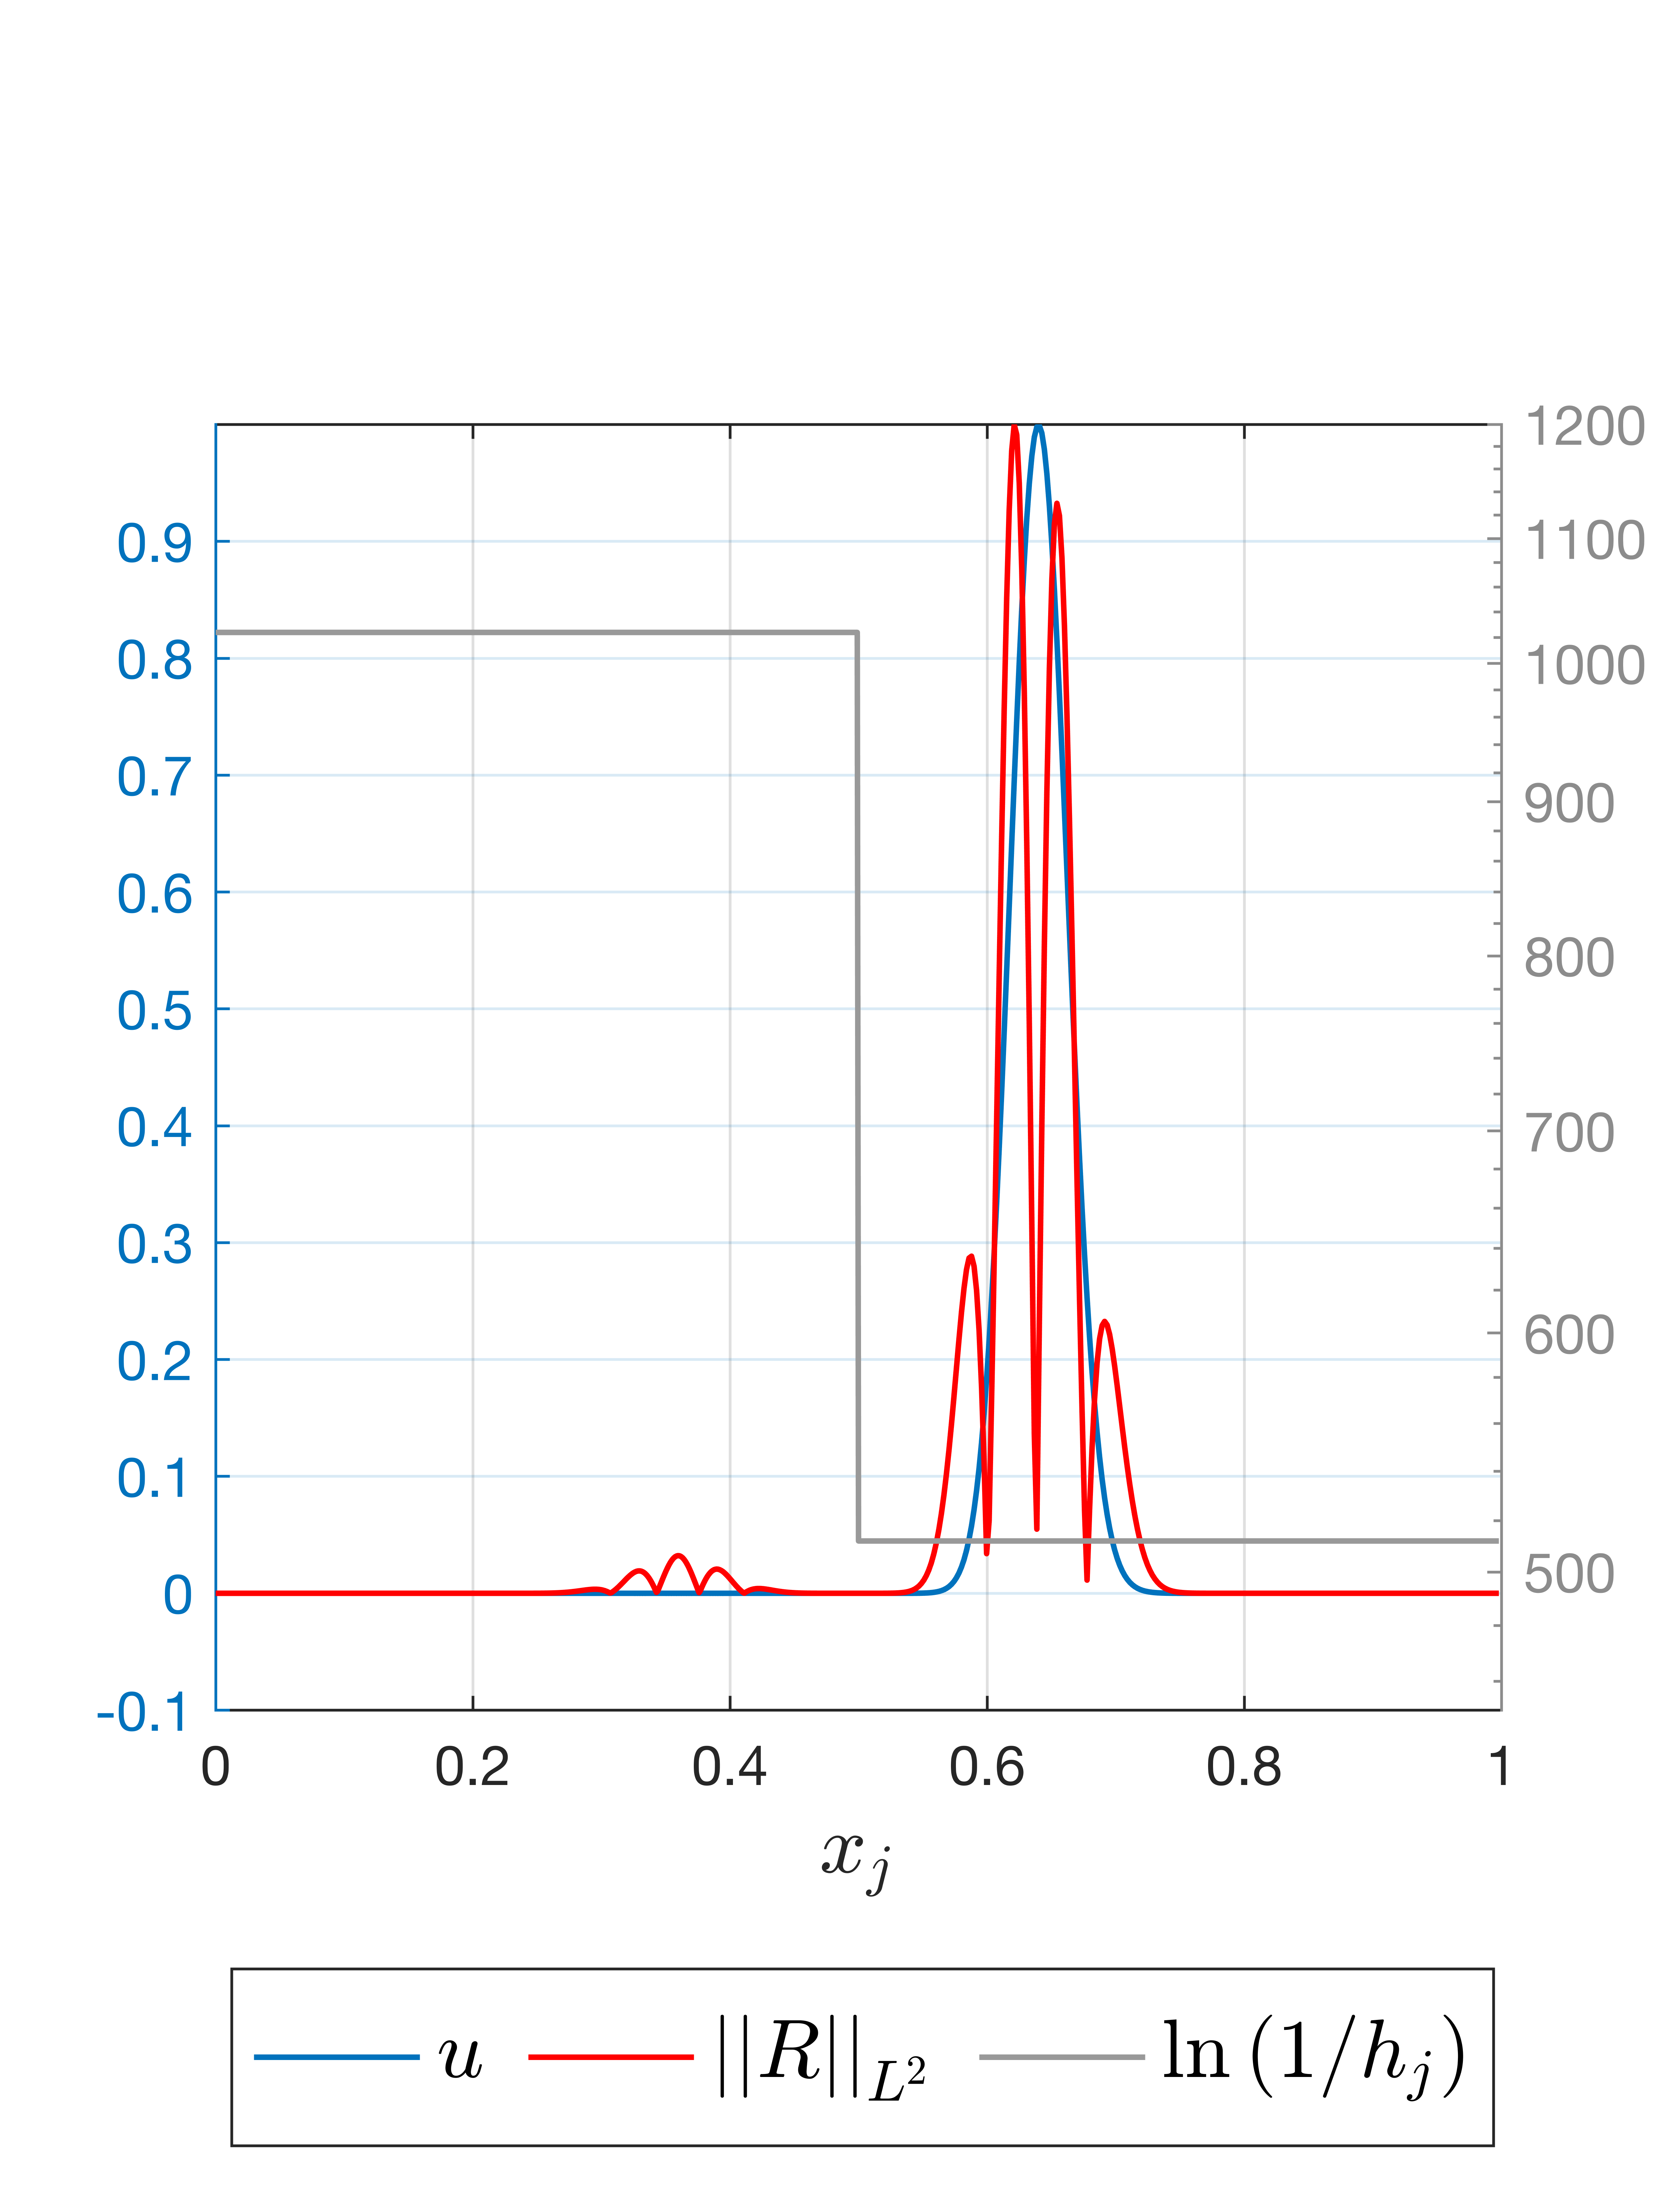
\includegraphics[width=\textwidth]{../figures/fig_CNCS_4000_para_1_legend}	
%		\caption{
%			After parasite formation.
%		}
%	\end{subfigure}
%	\begin{subfigure}[b]{.3\textwidth}
%	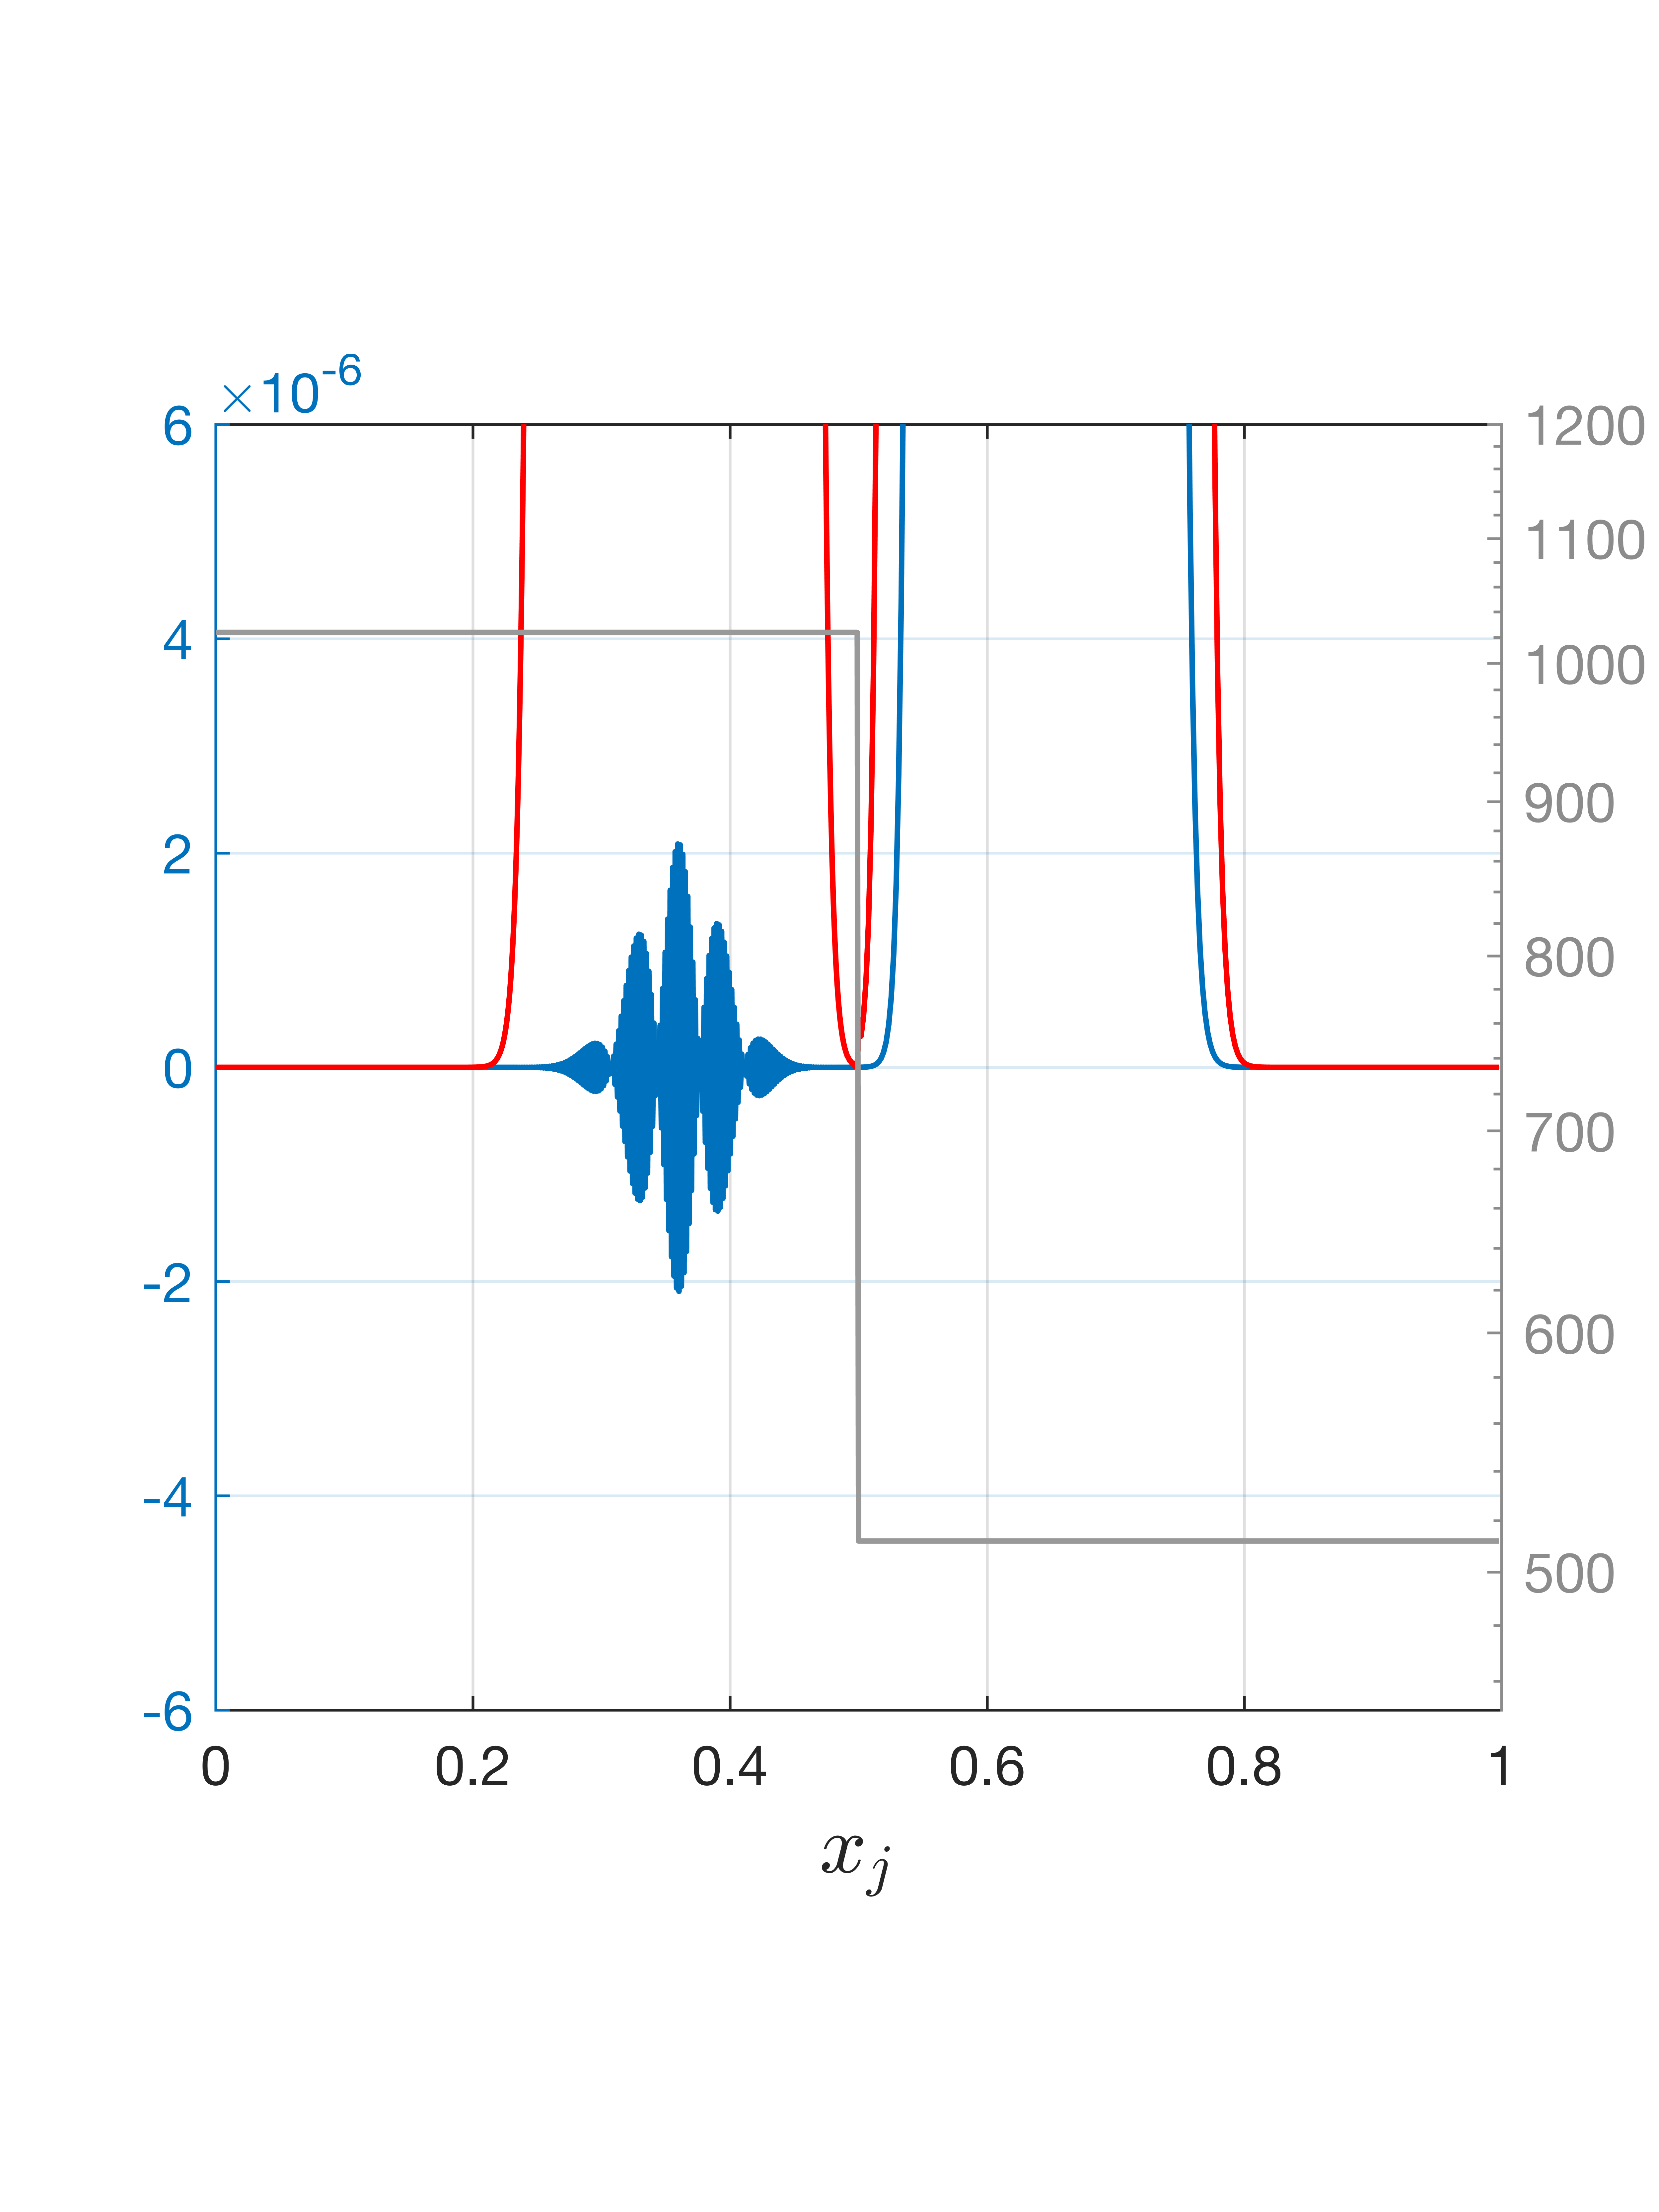
\includegraphics[width=\textwidth]{../figures/fig_CNCS_4000_para_1_zoom}	
%	\caption{
%		Magnified Parasite.
%	}
%\end{subfigure}
%	\caption{A parasitic wave which occurs to due an abrupt mesh change.  We use a CNCS scheme on a grid given by (\ref{eq_grid_spacing_piecewise_nonu}) and a temporal-to-spatial step coupling of $\tau=\frac{h}{10}$.  We plot the solution and the normalized $\leb{2}$-norm of the local residual (\ref{eq_reconstruction_gen_cons}) before and after parasite formation.  The parasitic wave is the highly oscillatory wave in the right-most plot, which is zoomed in.  Notice that it is moving in the opposite direction from the solution. Such parasites can arise when implementing adaptivity and can rapidly pollute the computation. Notice that the residual detects and tracks the parasite.}
%	}
%\end{figure}

In Fig.\ref{fig:CNCS_parasite} we see a parasite, which is the highly oscillatory wave-train shown in the bottom left plot.  Notice that it travels in the opposite direction compared to the initial condition.    Parasitic waves can rapidly pollute the computation.     Notice that the bound we have constructed using Defns. \ref{defn_temp_rec} and \ref{defn_spatio-temporal reconstruction} is able to detect the parasitic wave.  The reader should note that implementing adaptivity in the presence of an existing grid discontinuity may exacerbate parasite formation and propagation.


\section{Adaptive experiments}\label{sec:adaptive_implementation}
In  this section we discuss practical implementation details for the solution of (\ref{eq_1d_gen_cons_law}) in an adaptive context.   We describe the setup we use to test the suitability of (\ref{eq_reconstruction_gen_cons}) as a criterion for mesh adaptivity in 1D and we compare and contrast the results produced from the adaptive simulation with results produced from a uniform grid.

We begin by  presenting the adaptive algorithm we use.  Firstly, we will explain how we facilitate the comparison of the adaptive numerical simulation with the uniform one and then we present the  marking and the refinement/coarsening strategies.

\subsection{Adaptive Algorithm}
Our adaptive algorithm is of SOLVE $\to$ ESTIMATE $\to$ MARK $\to$ REFINE type.

\begin{Rem}[Maximum number of refinements]
For the purposes of this paper we allow a maximum of  four  refinement levels relative to the initial, uniform triangulation. 
\end{Rem}
There are potentially several ways to compare the performance of a numerical solution on a uniform and an adaptive mesh.  In this case we will use what we will refer to as an \textit{equivalent uniform mesh}.
\begin{Defn}[Equivalent Uniform Mesh]  \label{defn:equiv_uniform_mesh} We define a uniform mesh to be equivalent to an adaptive mesh if it has the same cumulative number of degrees of freedom, which we define as
	\begin{equation}
\sum_{n=0}^{N}N_{dof}\qp{t^n}.
	\end{equation}
\end{Defn}
 We find this number by firstly running the simulation on the adaptive mesh and recording the number of \text{dof} at each time-step.  We then average this over the number of time steps and set the resulting value to be the number of degrees of freedom for the equivalent uniform mesh.

\subsection{Marking}
The criterion for marking cells for refinement/coarsening is based is a maximum strategy.  We refine cells wherein  the value of the local indicator is larger than some multiple of the maximum value of the local residual and coarsen cells where it is lower.  We  do nothing in cases where the local value of the indicator falls in between the two values.  Lastly, we do not coarsen a cell marked if its sibling is marked for   refinement at the same time-step.

This strategy is described in detail in  \cite[\S1.5]{schmidt2005design} and it is modified for time-dependent problems for the purposes of these experiments.  Briefly, let $\eta_S$ denote the local residual term $\Norm{R}_{\leb
{2}\qp{I_j}}$ in a 'cell' $S:=I_j=\qb{x_j, x_{j+1}}$ for $S\in S_K$, where $S_K$ is the initial parent triangulation.  We set two predefined tolerances $\gamma_r$ and $\gamma_c$ for refining and coarsening respectively.  We mark a cell for refinement if
\begin{equation}
\eta_S \geq \gamma_r \max_{S'} \eta_{S'}, \, S' \in S_k
\end{equation}
and we mark for coarsening coarsen if 
\begin{equation}
\eta_S \leq \gamma_c \max_{S'} \eta_{S'}, \, S' \in S_k.
\end{equation}
The reader should note that there are several ways of choosing $\gamma_c$ and $\gamma_r$.  We chose them empirically as $\gamma_c = .05e-10$ and $\gamma_r= 0.5e-8$.  We summarize the marking-refinement/coarsening process in Algorithm \ref{Algorithm_MM_adaptivity}.

\begin{algorithm}[H]
	\caption{Mesh Adaptivity}\label{Algorithm_MM_adaptivity}
	\begin{algorithmic}
		\State $\textbf{Require: }$ Maximum number of refinement levels relative to initial triangulation, refinement parameter $\gamma_r$ and coarsening parameter $\gamma_c$.
		\While{$t^n<T$}
		\State set $S^{\qp{0}}_K=S_k$, the initial grid for the time-step  $t^n$.
		\State Solve (\ref{eq_conservation_form})  on $S^{\qp{0}}_K$ and compute the local indicator $\eta_S$ for all $S\in S^{\qp{0}}_K$.  
		\State Set $\eta_{\max}:=\max_{S'\in\mathcal{S}_k}\eta_{S'}$.
		\For{$S\in S_K^{\qp{0}}$}
		\If  {$\eta_S >\gamma_r \eta_{\max}$}
		\State Mark $S$ for refiment
		\EndIf
		\EndFor
		\For{$S\in S_K^{\qp{0}}$}
		\If  {$\eta_S <\gamma_c \eta_{\max}$}
		\If {$S\notin S_K$ \textbf{and} the siblings of $S$ are not marked for refinement}
		\State Mark $S$ for coarsening
		\EndIf
		\EndIf
		\EndFor
		\For {$S\in S^{\qp{0}}_K$}
		\If {$S$ is marked for refinement}
		\State Create two children of $S$
		\State Prolong $\vec{U}$ over $S$ and assign corresponding values to children nodes
		\State Prolong the grid $\bracegs{x_j}$ assigning corresponding values to children nodes
		\Else \textbf{if} {$S$ is marked for coarsening}
		\State Restrict $\vec{U}$ by assigning the relevant values from $S$ and its sibling to their parent
		\State Restict the grid $\bracegs{x_j}$ by assigning corresponding values from $S$ and its sibling to their parent
		\State Delete $S$ and its sibling
		\EndIf
		\EndFor
		\State Recompute both the error and the bound from (\ref{eq_prelim_bound}) and record them as the values for  time step $t^n$
		\State  \textbf{do} $n:=n+1$
		\EndWhile
		\State $\textbf{end}$
	\end{algorithmic}
\end{algorithm}

\/*
\While {($\mathcal{E}_{max}>\text{tol}$ and $n<n_{cycles}$)} 
\For{\texttt{$K\in \mathcal{T}_i$}}
\If{($\mathcal{E}_K>\gamma \mathcal{E}_{max}$ and $K$ has not been refined the maximum number of times)}
\State Mark $K$ for refinement
\EndIf
\EndFor
\State set $n=n+1$.
\State Refine all marked $K$ to obtain $T_i^{\qp{n+1}}$
\State Solve (\ref{eq_cons_law_1D_discrete}) on $\mathcal{T}_i^{\qp{n+1}}$ and calculate new $\mathcal{E}_{max}$
\EndWhile
\State Set $\mathcal{T}_{i+1}=\mathcal{T}_i^{\qp{n}}$
*/

\section{Adaptive experiments}\label{sec:adaptive_experiments}
In this section we describe the numerical experiments we run to test the a posteriori bounds as criteria for adaptivity.  We use two different problems: a linear advection problem with a discontinuous initial condition and periodic boundary conditions, and a shallow water dam-break problem with zero-neumann boundary conditions.  In this way we benchmark the performance of the indicator in more challenging settings than in previous sections. 
\begin{Rem}[Grid-spacing for the adaptive mesh] We start the simulations after having globally refined the entire grid the maximum allowable number of times.  Then, the indicator detects where this is excessive and coarsens locally.  This is the reason for  the steep decrease in the number of dof in the left plots in Fig. \ref{fig:FTBS_linadvect_adapt} and Fig. \ref{fig:SSP3WENO3_shw_dambreak_adapt}.
\end{Rem}
\begin{Rem}[Time-step for the adaptive mesh]  In order to maintain numerical stability, in the absence of an adaptive mechanism for the time-step, we  couple the time-step to the smallest spatial step present in the computation, to maintain numerical stability.
\end{Rem}

\subsection{Linear advection}
We run a benchmarking experiment experiment using the linear advection equation
\begin{equation}
u_t+u_x=0
\end{equation}
over a domain $\Omega = \qb{0,1}$ with $T=0.5$ using periodic boundary conditions and a discontinuous initial condition given by
\begin{equation}\label{eq_ic_step}
u_0\qp{x}=\begin{cases}
1\quad&\text{if}\quad \norm{x-.25}\leq 0 .125\\
0\quad&\text{if} \quad \norm{x-.25}>  0.125.
\end{cases}
\end{equation}
We discretise the problem using a Forward-Time Backward Space scheme given by (\ref{eq:FTBS}) for both the adaptive and the uniform case. The residual in this test case is constructed using a bilinear Lagrange interpolant.  Lastly, the grid-spacing for the equivalent uniform mesh (see Rem. \ref{defn:equiv_uniform_mesh}) is found to have 741 degrees of freedom, i.e. $0=x_0<\dots<x_{740}=1$.  The results are shown in Fig. \ref{fig:FTBS_linadvect_adapt}.

\begin{figure}[H]
\centering
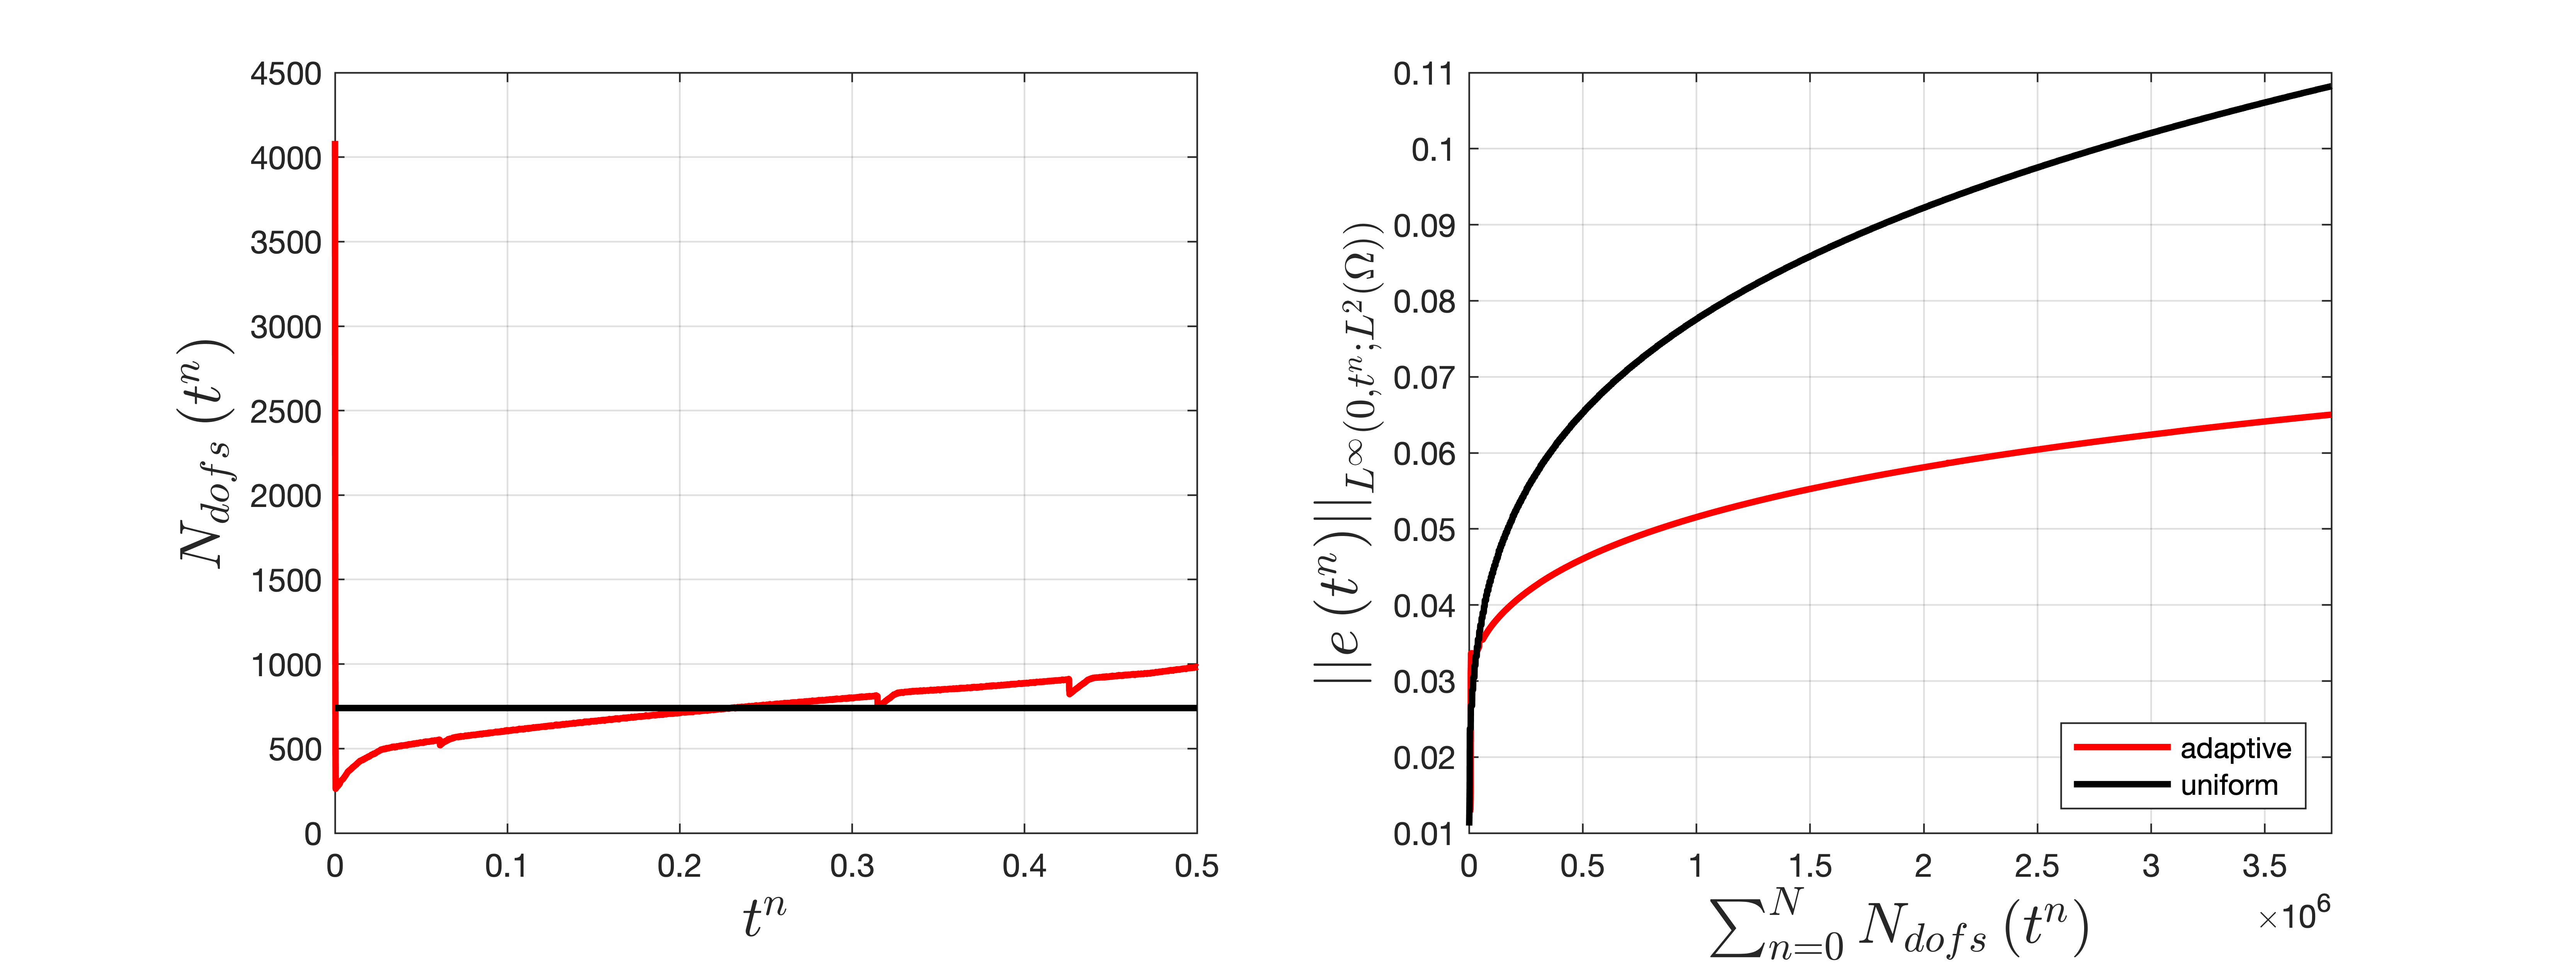
\includegraphics[width=\textwidth]{../figures/fig_FTBSplots_1x5_step_IC_P1_comparison_adaptONOFF}	
	\caption{\label{fig:FTBS_linadvect_adapt} An adaptive simulation of the linear advection equation with an FTBS discretization, periodic boundary conditions and a step initial condition given by (\ref{eq_ic_step}).  The simulation starts at the maximum allowable refinement level (we set this to be 4) with an initial (fine) grid with spacing $h=2^{-12}$ and a temporal step $\tau =\frac{2^{-10}}{10}$, which remains constant throughout the simulation. The equivalent uniform grid has $741$ degrees of freedom.  The indicator used in this case is a simple bilinear Lagrange indicator.  Notice that the indicator automatically coarsens the grid at the beginning of the simulation, resulting in a steep decrease in the number of decrease of freedom in parts of the domain which are away from the discontinuity. Also notice that the adaptive mesh compares favorably with an equivalent uniform grid as it consistently maintains a lower level of error throughout the major part of the simulation.}
\end{figure}

\/*
\begin{figure}[H]
	\begin{subfigure}[b]{.41\textwidth}
		\centering
		\resizebox{\linewidth}{!}{		\begin{tikzpicture}
			\begin{axis}[
			cycle list/Dark2,
			thin,
			%xmode=log,
			ymode=log,
			xlabel=$t^n$,
			ylabel=$ N_{dof}\qp{t^n}$,
			grid=both,
			minor grid style={gray!25},
			major grid style={gray!25},
			width=\linewidth,
			no marks,
			legend style={at={(1.,0)},anchor=south east},
			]
			\addplot+
			table[x=time_arr_ON,y=dofs_arr_ON, col sep=comma]{data/dofs_file_adapt.csv};
			%\addlegendentry{Adaptive grid};
			\addplot+
			table[x=time_arr_ON,y=dofs_arr_OFF, col sep=comma]{data/dofs_file_adapt.csv};
		%	\addlegendentry{Uniform grid};
			\end{axis}
			\end{tikzpicture}}
		\caption{\label{fig:FTBS_adapt_dofs}Dofs}
	\end{subfigure}
	\begin{subfigure}[b]{.41\textwidth}\label{fig:FTBS_adapt_error}
		\centering
		\resizebox{\linewidth}{!}{	\begin{tikzpicture}
			\begin{axis}[
			cycle list/Dark2,
			thin,
			%xmode=log,
			ymode=log,
			xlabel=$t^n$,
			ylabel=$\Norm{e}_{\leb{\infty}\qp{0,t^n;\leb{2}\qp{\W}}}$,
			grid=both,
			minor grid style={gray!25},
			major grid style={gray!25},
			width=\linewidth,
			no marks,
			legend style={at={(1.,0)},anchor=south east},
			]
			\addplot+
			table[x=time_arr_ON,y=error_arr_ON, col sep=comma]{data/error_file_adapt.csv};
			%\addlegendentry{Adaptive grid};
			\addplot+
			table[x=time_arr_ON,y=error_arr_OFF, col sep=comma]{data/error_file_adapt.csv};
		%	\addlegendentry{Uniform grid};
			\end{axis}
			\end{tikzpicture}}
		\caption{Error}
	\end{subfigure}
	\caption{\label{fig:FTBS_linadvect_adapts} An adaptive simulation of the linear advection equation with an FTBS discretization, periodic boundary conditions and a step initial condition given by (\ref{eq_ic_step}).  The simulation starts at the maximum allowable refinement level (we set this to be 4) with an initial (fine) grid with spacing $h=2^{-12}$ and a temporal step $\tau =\frac{2^{-10}}{10}$, which remains constant throughout the simulation. The equivalent uniform grid has $741$ degrees of freedom.  The indicator used in this case is a simple bilinear Lagrange indicator.  Notice that the indicator automatically coarsens the grid at the beginning of the simulation, resulting in a steep decrease in the number of decrease of freedom in parts of the domain which are away from the discontinuity. Also notice that the adaptive mesh compares favorably with an equivalent uniform grid as it consistently maintains a lower level of error throughout the major part of the simulation.}
\end{figure}
*/
\subsection{Shallow water equations}\label{subsec:shallow_water_tests}
In this case we conduct a numerical experiment to test the residual term $\vect{R}$ in (\ref{eq_bound}) as a local refinement criterion for the shallow water equations using a dam-break initial condition and free outflow conditions.  The model we test is given by
\begin{equation}\label{eq_model_SWE}
\begin{aligned}
\begin{array}{c}
\eta_t\\
\qp{\eta v}_t
\end{array}
\begin{array}{c}
+\\
+
\end{array}
\begin{array}{c}
\qp{\eta v}_x\\
\qp{\eta v^2+\frac{1}{2}g\eta^2}_x
\end{array}
\begin{array}{c}
=0\\
=0,
\end{array}
\end{aligned}
\end{equation}
equipped with the initial conditions
\begin{equation}
\begin{aligned}
h\qp{x,0}&=\begin{cases}
h_0\quad \text{for} \quad x\leq x_0\\
h_1\quad \text{for}\quad  x> x_0,
\end{cases}\\
v\qp{x,0}&=v_0\qp{x}.
\end{aligned}
\end{equation}
over a domain $\Omega=\qb{0, 32\pi}$ and $T\approxeq10$. We use
$v_0\qp{x,0} = 0$, $x_0 = 30$, $h_0=0.2$ and $h_1= 0.1$ for the
initial condition.  The initial fine mesh is given by $h=32\pi \times
2^{-14}$ and a constant time-step $\tau =\frac{32\pi \times 2^{-12}
}{10}$. We show an evolution of this solution in Fig. \ref{fig:SSP3WENO_shw_stills}. The equivalent uniform mesh is found to have 1622 degrees of freedom, i.e. $0=x_0<\dots<x_{1621}=32\pi$.  The benchmarking results are shown in Figure \ref{fig:SSP3WENO3_shw_dambreak_adapt}.


\begin{figure}[H]
	\begin{subfigure}[b]{.25\textwidth}
		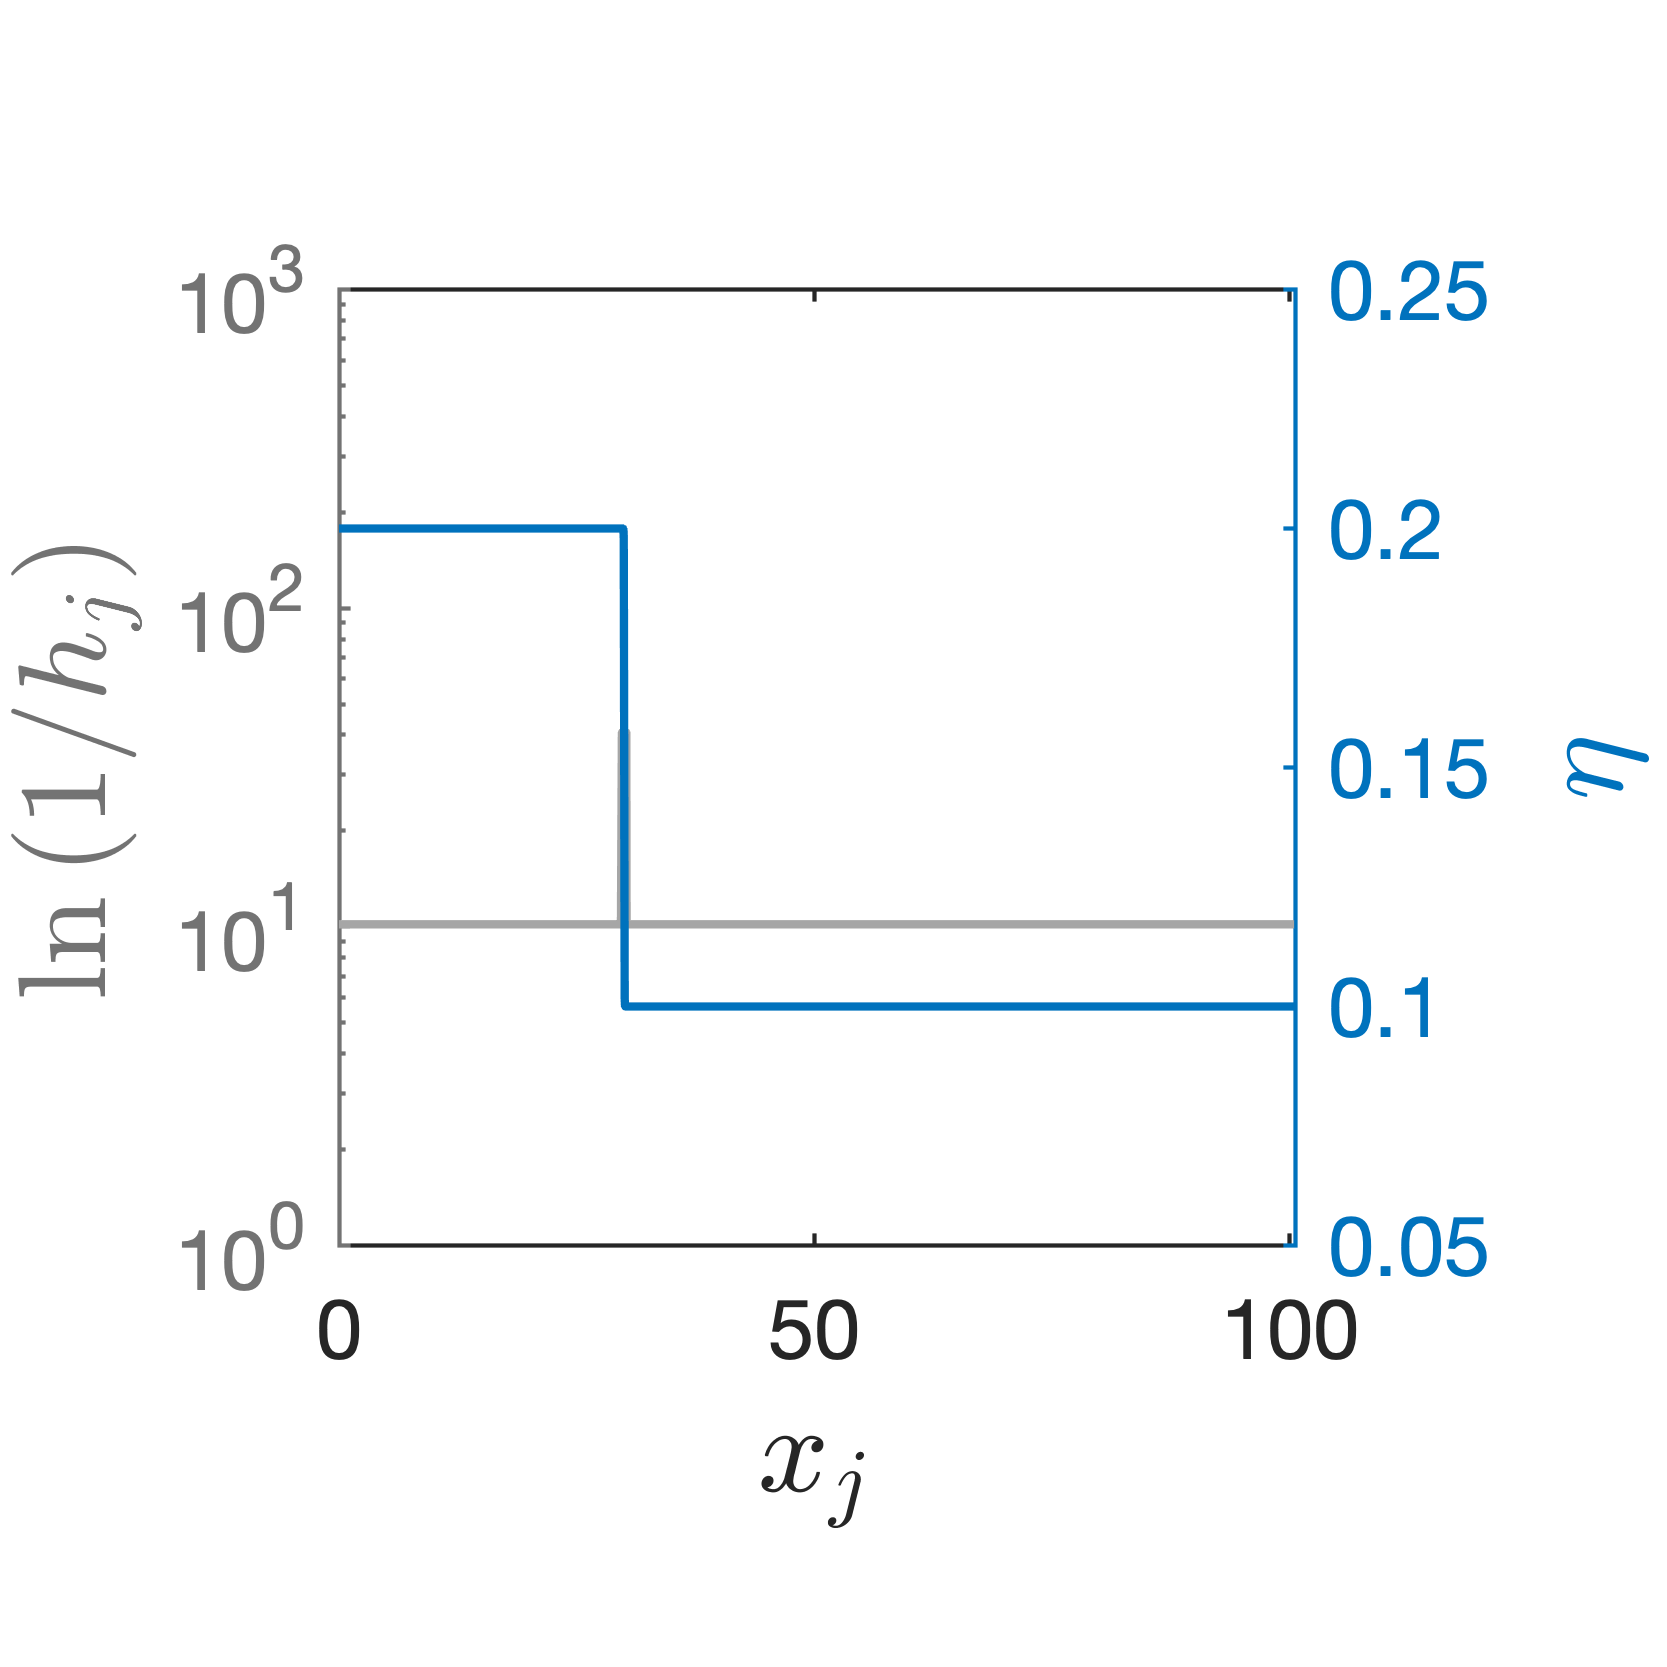
\includegraphics[width=\textwidth]{../figures/fig_shw_dambreakSHW_dambreak_RK3_WENO3_rec_3_fixed_gs_stills_1_adaptONOFF}	
		\caption{
			\label{fig_shw_dambreakSHW_dambreak_RK3_WENO3_rec_3_fixed_gs_stills_1_adaptONOFF}
		}
	\end{subfigure}
	\begin{subfigure}[b]{.25\textwidth}
	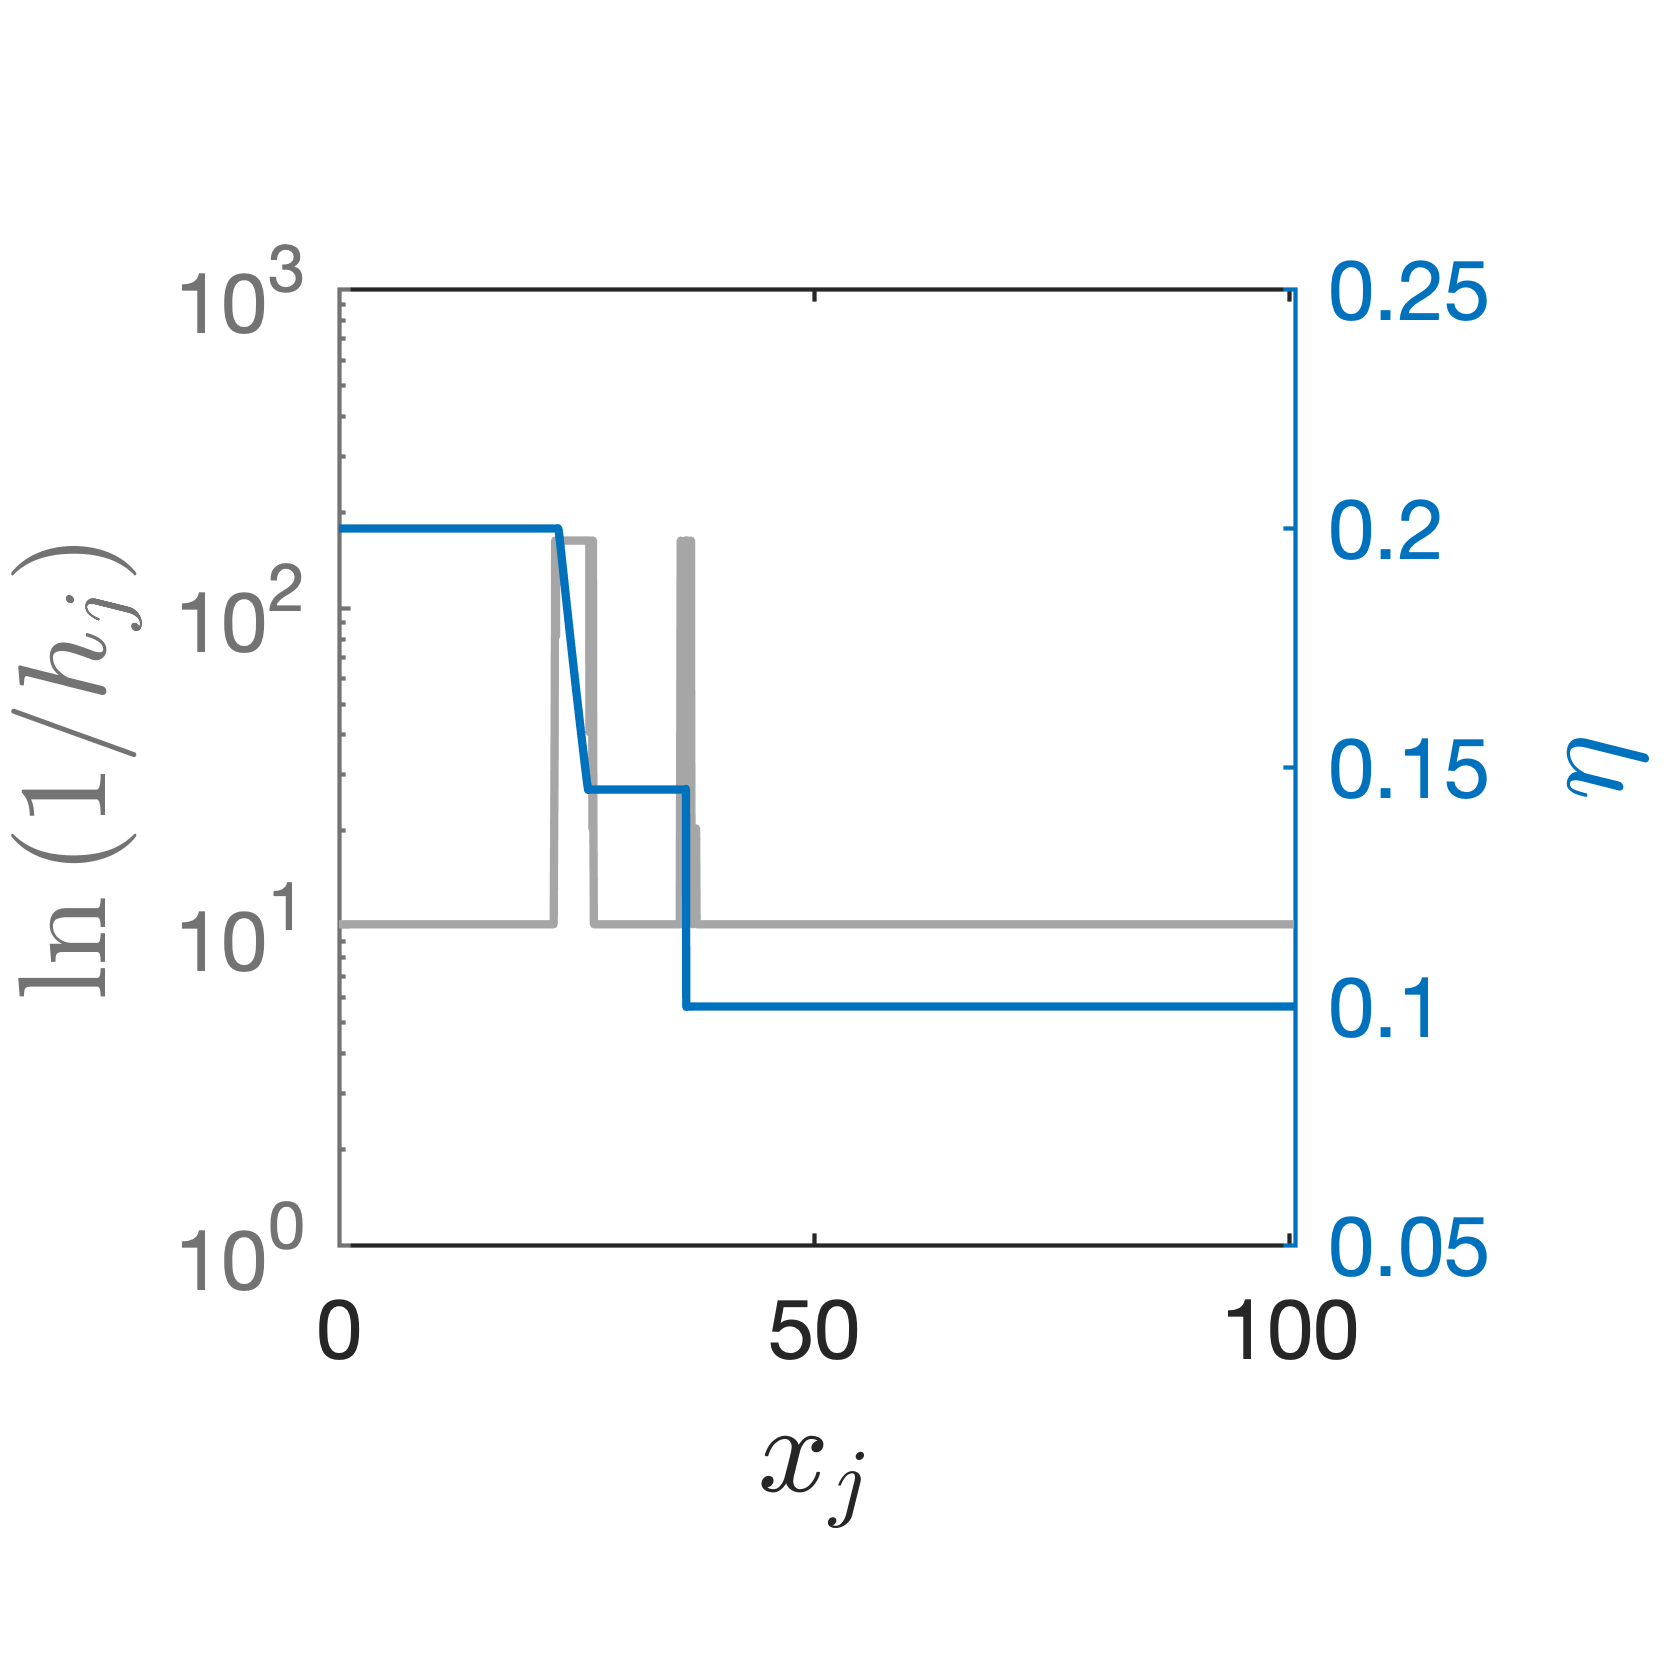
\includegraphics[width=\textwidth]{../figures/fig_shw_dambreakSHW_dambreak_RK3_WENO3_rec_3_fixed_gs_stills_2001_adaptONOFF}	
	\caption{
		\label{fig_shw_dambreakSHW_dambreak_RK3_WENO3_rec_3_fixed_gs_stills_2001_adaptONOFF}
	}
\end{subfigure}
	\begin{subfigure}[b]{.25\textwidth}
	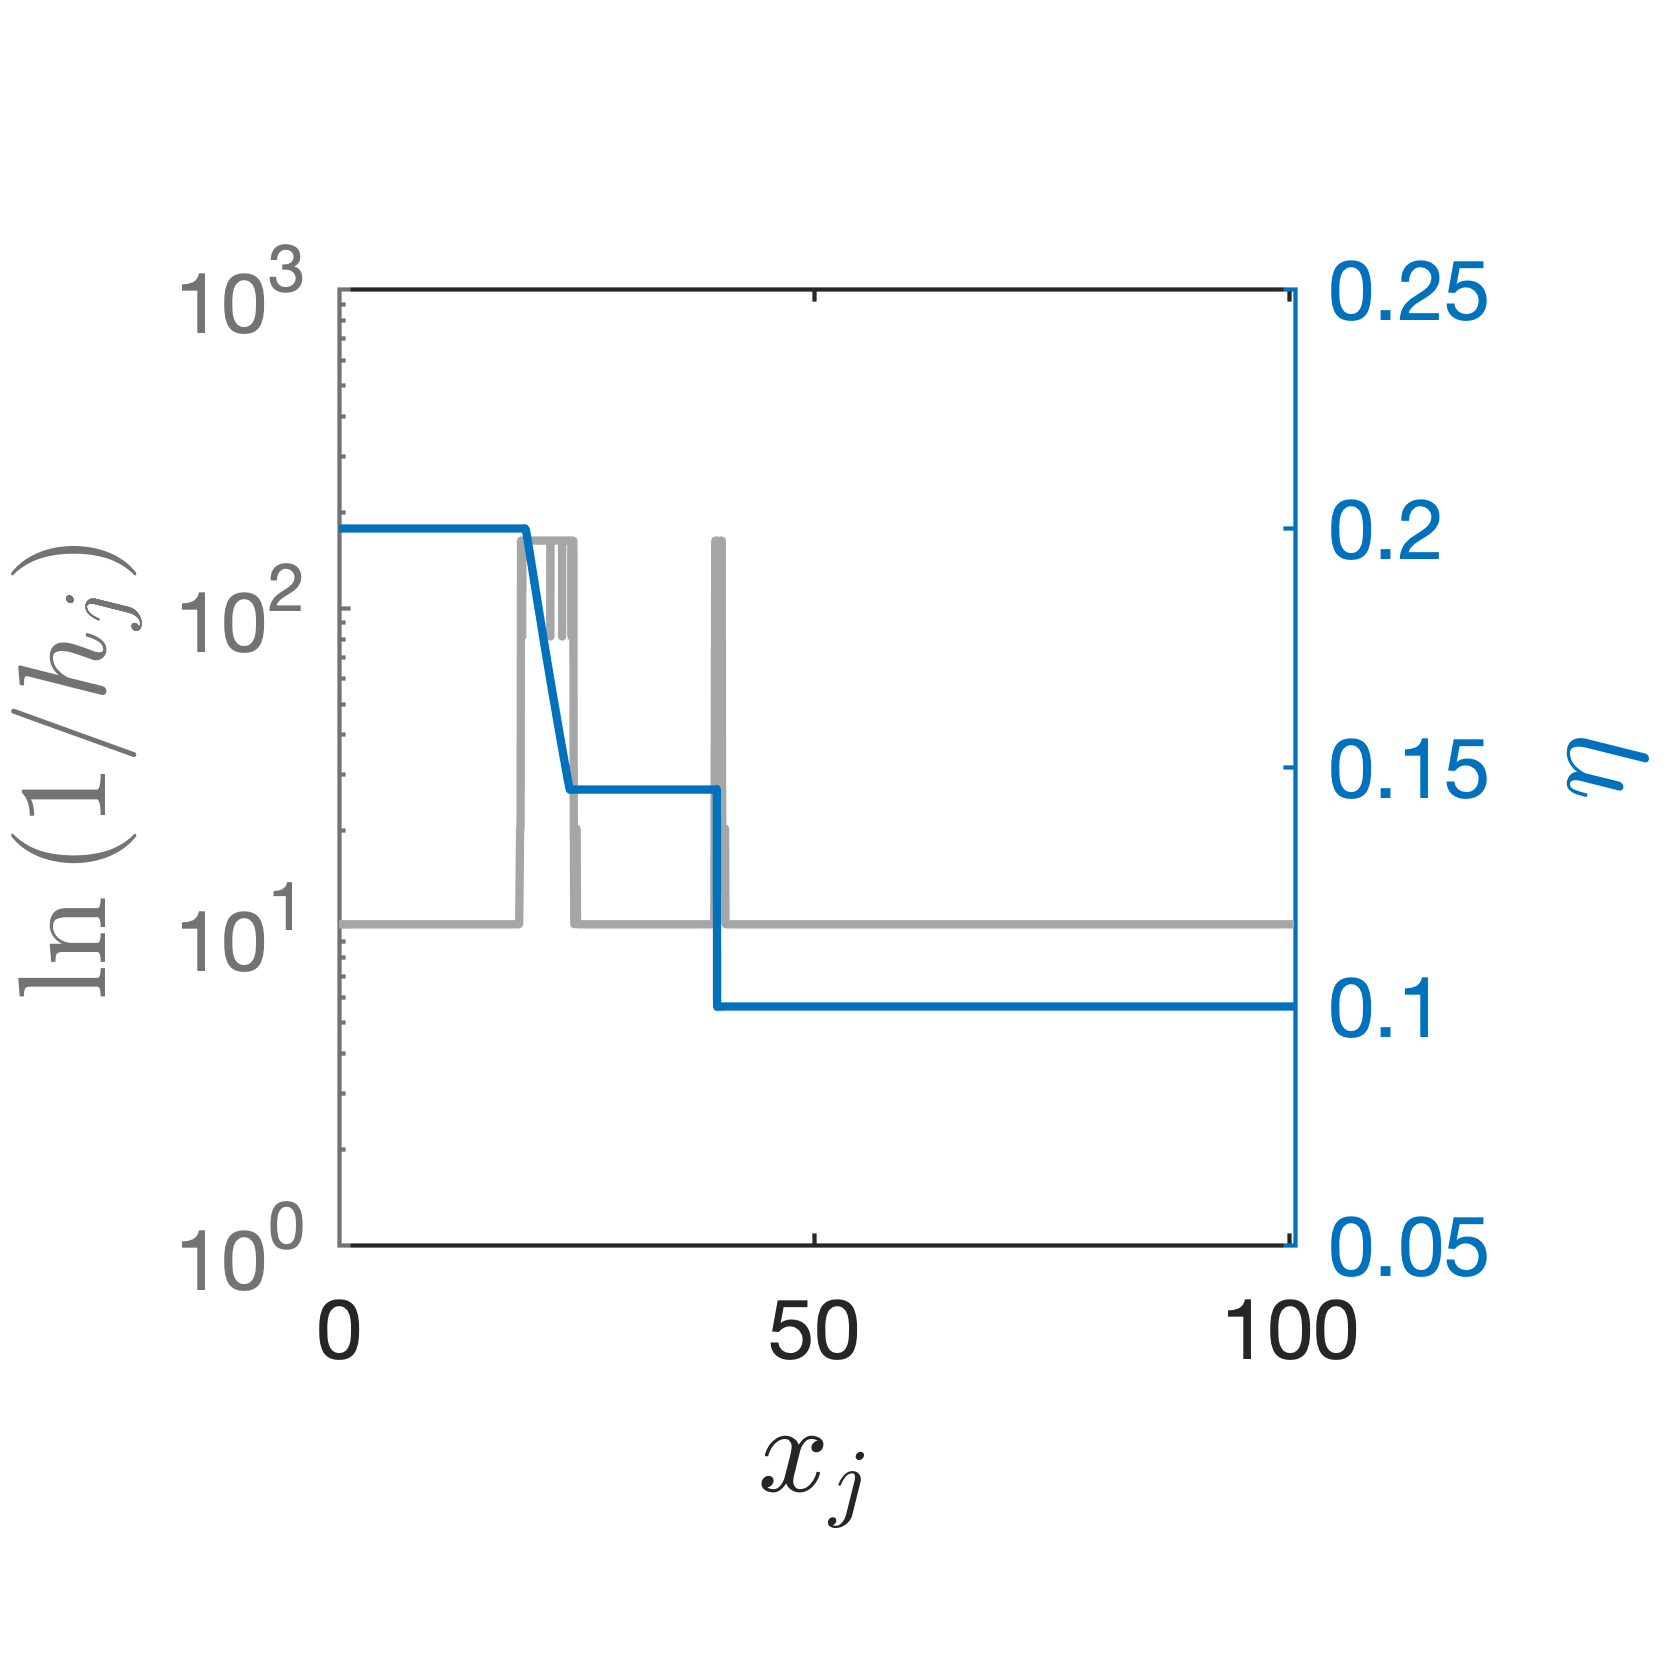
\includegraphics[width=\textwidth]{../figures/fig_shw_dambreakSHW_dambreak_RK3_WENO3_rec_3_fixed_gs_stills_3001_adaptONOFF}	
	\caption{
		\label{fig_shw_dambreakSHW_dambreak_RK3_WENO3_rec_3_fixed_gs_stills_3001_adaptONOFF}
	}
\end{subfigure}
	\\
\begin{subfigure}[b]{.25\textwidth}
	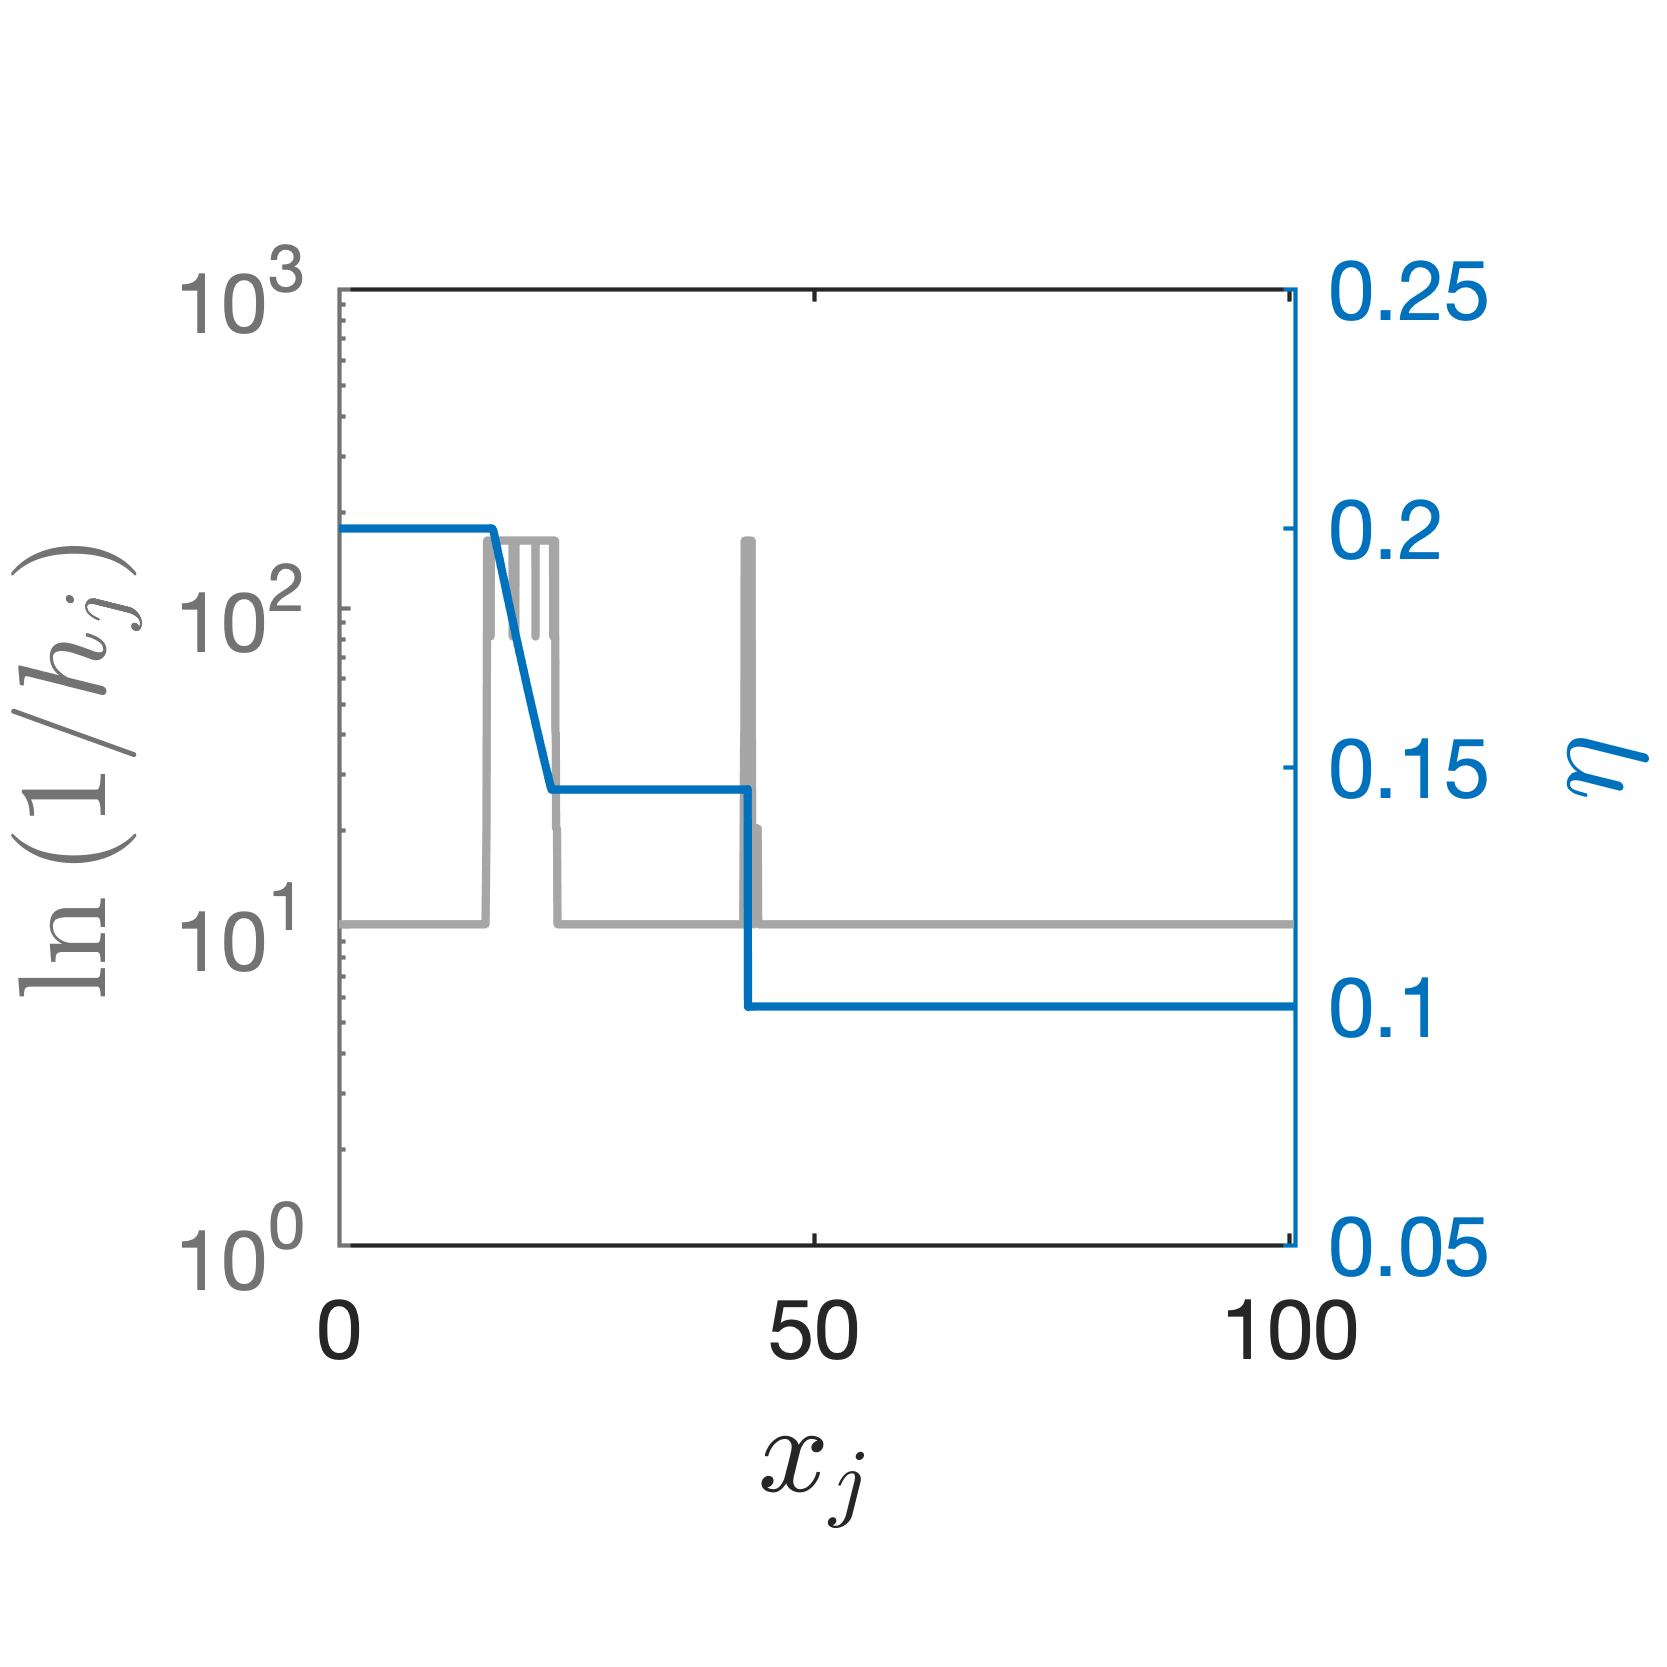
\includegraphics[width=\textwidth]{../figures/fig_shw_dambreakSHW_dambreak_RK3_WENO3_rec_3_fixed_gs_stills_4001_adaptONOFF}	
	\caption{
		\label{fig_shw_dambreakSHW_dambreak_RK3_WENO3_rec_3_fixed_gs_stills_4001_adaptONOFF}
	}
\end{subfigure}
\begin{subfigure}[b]{.25\textwidth}
	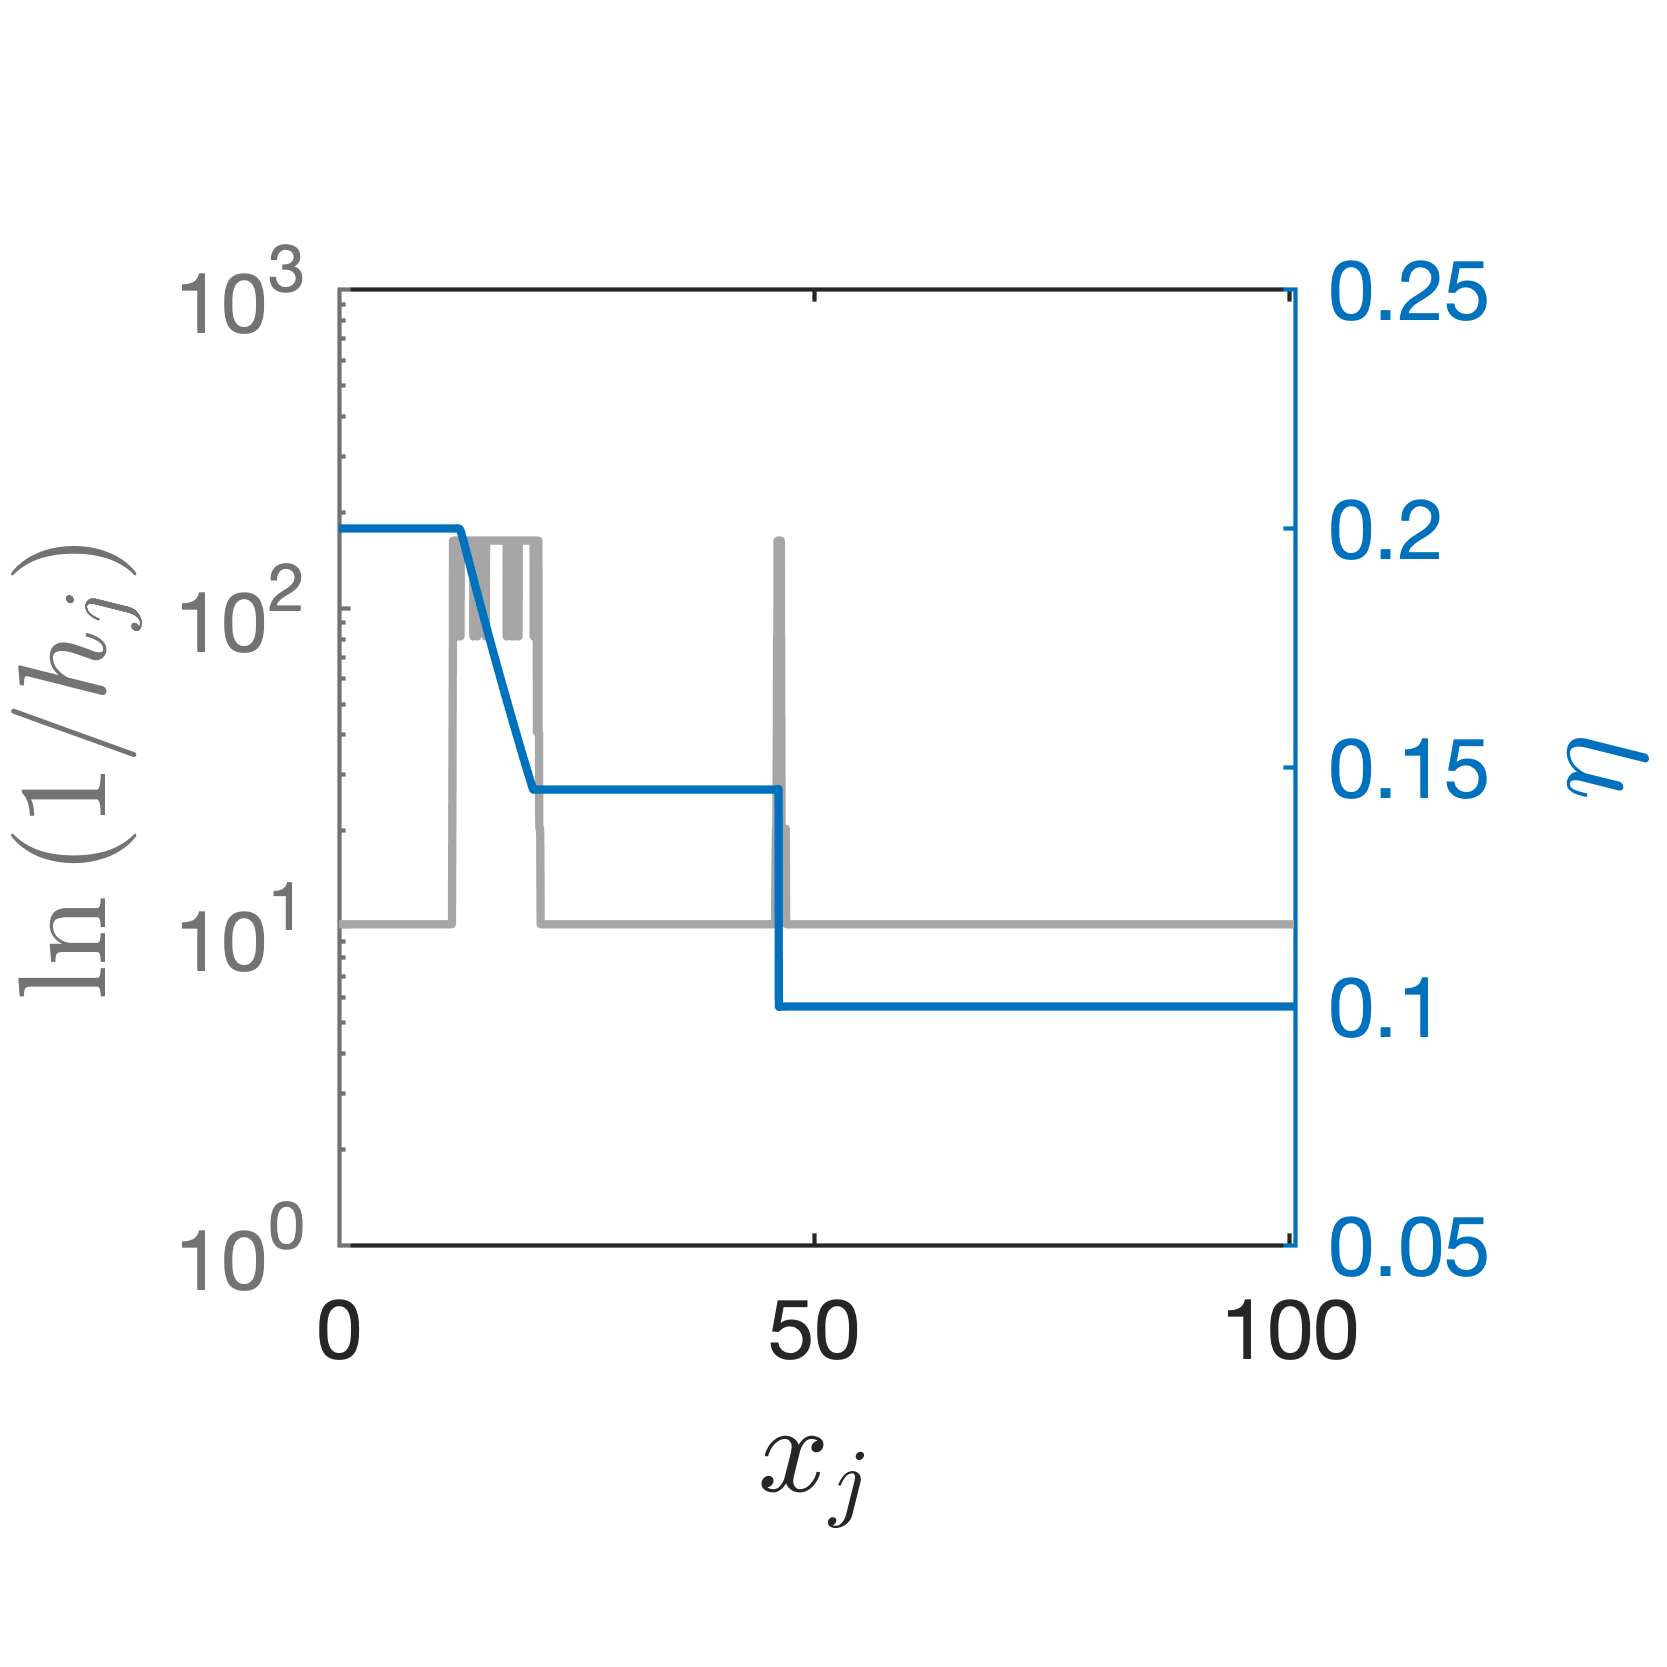
\includegraphics[width=\textwidth]{../figures/fig_shw_dambreakSHW_dambreak_RK3_WENO3_rec_3_fixed_gs_stills_5001_adaptONOFF}	
	\caption{
		\label{fig_shw_dambreakSHW_dambreak_RK3_WENO3_rec_3_fixed_gs_stills_5001_adaptONOFF}
	}
\end{subfigure}
\begin{subfigure}[b]{.25\textwidth}
	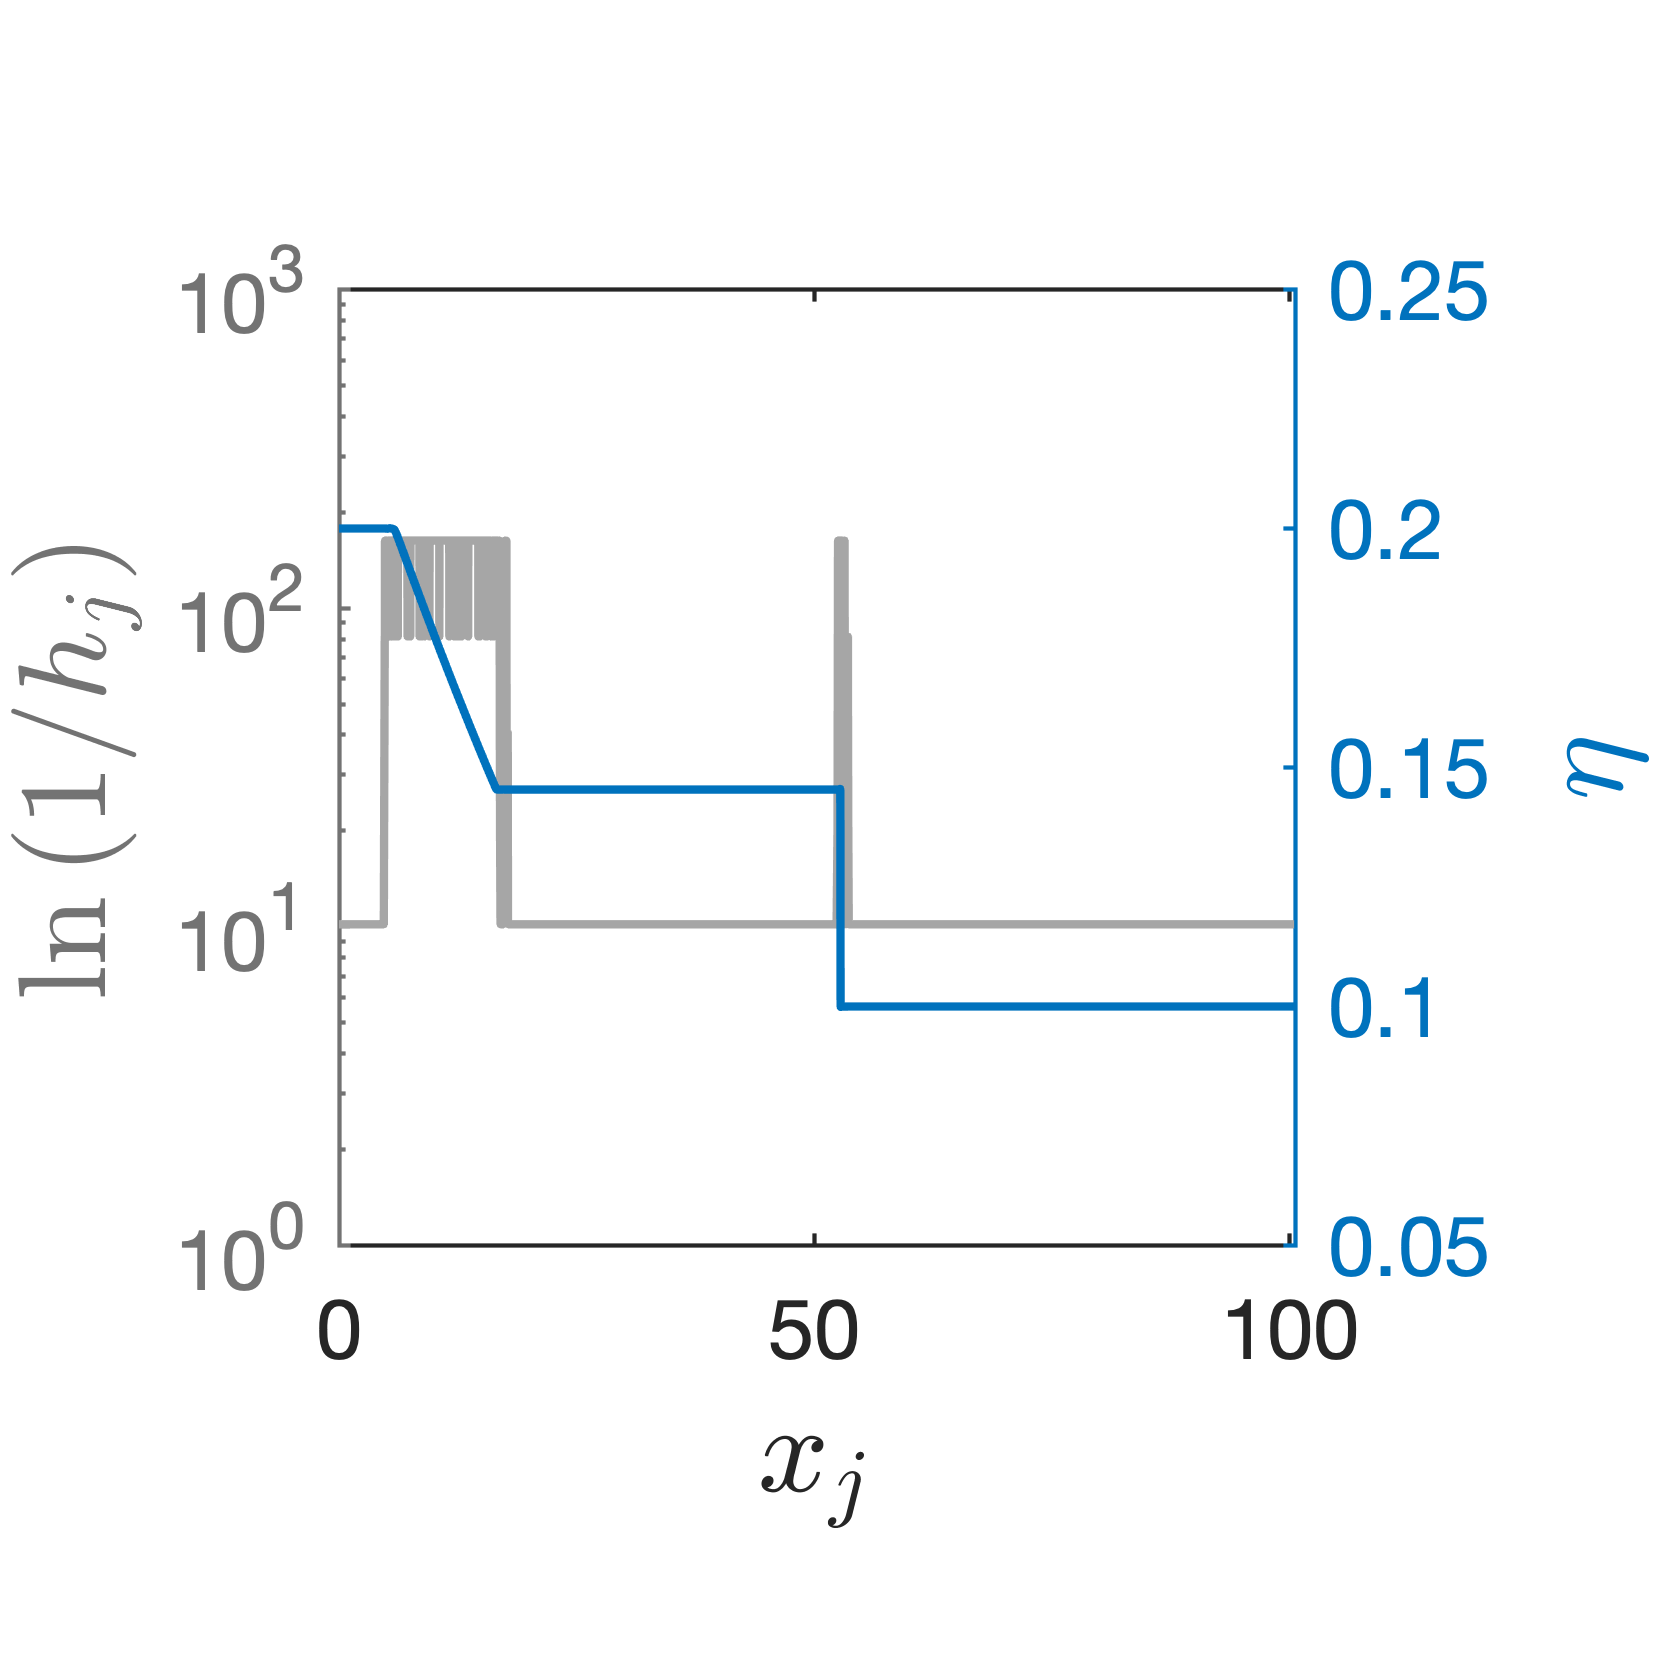
\includegraphics[width=\textwidth]{../figures/fig_shw_dambreakSHW_dambreak_RK3_WENO3_rec_3_fixed_gs_stills_7001_adaptONOFF}	
	\caption{
		\label{fig_shw_dambreakSHW_dambreak_RK3_WENO3_rec_3_fixed_gs_stills_7001_adaptONOFF}
	}
\end{subfigure}
	\caption{\label{fig:SSP3WENO_shw_stills} Evolution of the surface elevation (blue line) for the shallow water dam break problem, using and SSP3-WENO3 spatio temporal discretization.  The logarithm of the reciprocal of the local grid-spacing is overlaid with a grey line. We use a Hermite-WENO3 spatio-temporal reconstruction to construct the residual, $R$ (see (\ref{eq_reconstruction_gen_cons})). The simulation starts at the maximum allowable refinement level with a uniform grid with spatial step $h=32\pi \times 2^{-14}$ and a temporal step $\tau =\frac{32\pi\times2^{-12}}{10}$ which remains constant throughout the simulation.  Notice that the residual accurately detects regions where refinement is required - such as in the vicinity of the shock and the rarefaction) and where coarsening is appropriate.}
\end{figure}


\begin{figure}[H]
\centering
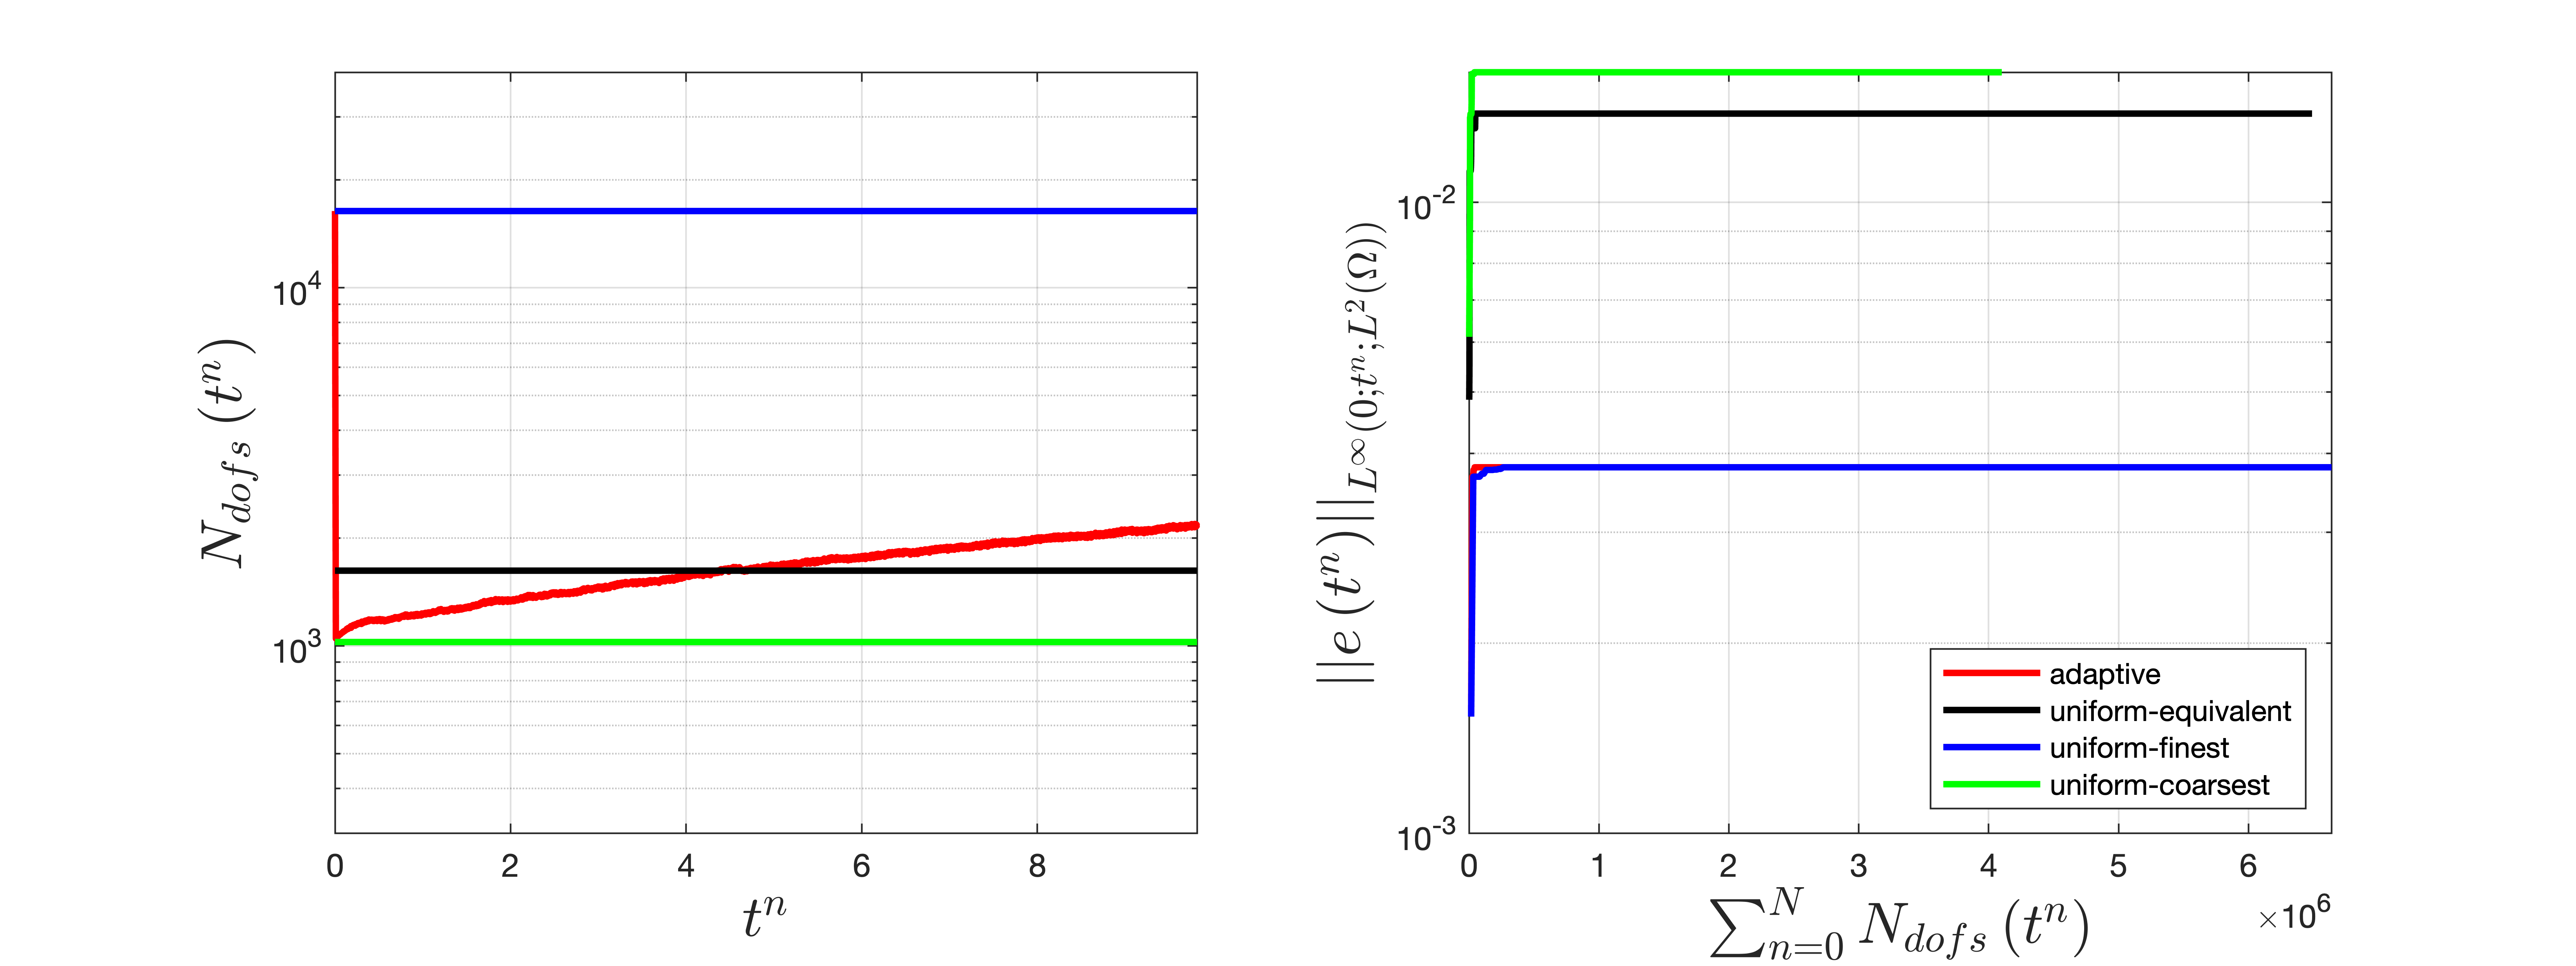
\includegraphics[width=\textwidth]{../figures/fig_SHW_dambreak_RK3_WENO3_rec_3_fixed_gsplots_1x5_shw_dambreak_comparison_adaptONOFF}	
	\caption{\label{fig:SSP3WENO3_shw_dambreak_adapt} An adaptive simulation of the shallow water equations for the dam-break problem using an SSP3-WENO3 discretization and free outflow boundary conditions.  The simulation starts at the maximum allowable refinement level with a uniform grid with $h=32\pi \times 2^{-14}$ and a temporal step $\tau =\frac{32\pi\times2^{-12}}{10}$ which remains constant throughout the simulation. The equivalent uniform grid has $1622$ degrees of freedom.  The residual is constructed using a bilinear Lagrange indicator.  Notice that the indicator automatically coarsens the grid at the beginning of the simulation, resulting in a steep decrease in the number of freedom away from the discontinuity. The behaviour in the adaptive case is almost identical with that of the finest resolution despite the considerable difference in degrees of freedom (the two results are almost entirely coincident on the right plot).  This is because, for this problem, the features of refinement interest are concentrated in small areas, allowing for good resolution with relatively few degrees of freedom. }
\end{figure}

\section{Conclusions}\label{sec:conclusion}
The main contribution from this article is a framework for constructing reliable, optimal a posteriori error estimates for classes of Finite Difference schemes, which have not received as much attention in the context of a posteriori estimates as FE and FV.   The framework is generally applicable: it does not depend on the specific choice of the underlying FD scheme.

The methodology incorporates both the numerical solution and information from the FD scheme itself, thereby facilitating the construction of high order a aposteriori estimates using reconstruction techniques. This is  a desirable property as it enables the user to construct optimal estimates for high order FD schemes.  
At the moment, this is limited to order three on account of the approach taken for the temporal component. Despite this limitation, the method for exceeding order three has been delineated.  We used this with success for the spatial component.  This will be incorporated for the temporal component  in future work.



We demonstrate that the  obtained estimates possess desirable characteristics using a range of numerical tests with both linear and nonlinear, scalar and vectorial examples.  In these tests, the estimates show optimal convergence characteristics while the solution is smooth, but break down in the presence of shocks.  This is because they contain terms which blow up when shocks appear and as the mesh size goes to zero.

We also show that the residuals constructed using the methodology we propose can be used as local mesh refinement criteria with favourable results relative to equivalent uniform grids.  We demonstrate this using a scalar linear problem and a nonlinear system of conservation laws in one dimension.

The behaviour in the post shock regime, pertaining not only to optimality, but indeed to convergence, remains a future challenge.


 
  \/*

 \begin{figure}[H]
 	\begin{subfigure}[b]{.4\textwidth}
 		\centering
 		\resizebox{\textwidth}{!}{	\begin{tikzpicture}
 			\begin{axis}[
 			no markers,
 			every axis plot/.append style={semithick},
 			cycle list/Dark2,
 			thin,
 			%xmode=log,
 		%	ymode=log,
 		axis y line*=left,
 			xlabel=$x_j$,
 		%	ylabel=y1,
 			ymin=-0.1,
 			ymax = 1.0,
 		%	grid=both,
 			minor grid style={gray!25},
 			major grid style={gray!25},
 			width=\linewidth,
 			no marks,
 			legend columns = 2,
 			legend style={at={(1,-0.3)},anchor=south west},
 			]
 			\addplot+[blue]
 			table[x=x_CNCS_para,y=u_arr_CNCS_para, col sep=comma]{data/error_file_para_advect_20.csv};
 			%	\addlegendentry{Adaptive grid};
 			\addplot+[red]
 			table[x=x_CNCS_para,y=bound_arr_CNCS_para, col sep=comma]{data/error_file_para_advect_20.csv};
 		%	\addplot+
 		%	table[x=x_CNCS_para,y=spacing_arr_CNCS_para, col sep=comma]{data/error_file_para_advect_20.csv};
 			%	\addlegendentry{Uniform fine grid};
 			\end{axis}
 			\begin{axis}[
 				no markers,
 			every axis plot/.append style={semithick},
 			cycle list/Dark2,
 			thin,
 			%xmode=log,
 				ymode=log,
 			axis y line*=right,
 				ymin = 450,
 			ymax = 1200,
 			xlabel=$x_j$,
 		%	ylabel=y2,
 		%	grid=both,
 			minor grid style={gray!25},
 			major grid style={gray!25},
 			width=\linewidth,
 			no marks,
 			legend columns = 2,
 			legend style={at={(1,-0.3)},anchor=south west},
 			]
 		%	\addplot+
 		%	table[x=x_CNCS_para,y=u_arr_CNCS_para, col sep=comma]{data/error_file_para_advect_20.csv};
 			%	\addlegendentry{Adaptive grid};
 		%	\addplot+
 	%		table[x=x_CNCS_para,y=bound_arr_CNCS_para, col sep=comma]{data/error_file_para_advect_20.csv};
 				\addplot+
 				table[x=x_CNCS_para,y=spacing_arr_CNCS_para, col sep=comma]{data/error_file_para_advect_20.csv};
 			%	\addlegendentry{Uniform fine grid};
 			\end{axis}
 			\end{tikzpicture}}
 		\caption{Before parasite forms}
 	\end{subfigure}
 		\begin{subfigure}[b]{.4\textwidth}
 		\centering
 		\resizebox{\textwidth}{!}{	\begin{tikzpicture}[spy using outlines ={magnification=2, rectangle, size = 1cm,blue, connect spies}]
 			\begin{axis}[
 				no markers,
 			every axis plot/.append style={semithick},
 			cycle list/Dark2,
 			thin,
 			%xmode=log,
 			%	ymode=log,
 			axis y line*=left,
 		%	xlabel=$x_j$,
 			%ylabel=y1,
 			ymin=-0.1,
 			ymax =1,
 		%	grid=both,
 			minor grid style={gray!25},
 			major grid style={gray!25},
 			width=\linewidth,
 			no marks,
 			legend columns = 2,
 			legend style={at={(1,-0.3)},anchor=south west},
 			]
 			\addplot+[blue]
 			table[x=x_CNCS_para,y=u_arr_CNCS_para, col sep=comma]{data/error_file_para_advect_4000.csv};
 			%	\addlegendentry{Adaptive grid};
 			\addplot+[red]
 			table[x=x_CNCS_para,y=bound_arr_CNCS_para, col sep=comma]{data/error_file_para_advect_4000.csv};
 			\coordinate (c1) at (axis cs: 0.358, 0.0);
 			\coordinate (c2) at (axis cs: 0.25, 0.5);
 			\spy on (c1) in node at (c2);
 			%	\addplot+
 			%	table[x=x_CNCS_para,y=spacing_arr_CNCS_para, col sep=comma]{data/error_file_para_advect_20.csv};
 			%	\addlegendentry{Uniform fine grid};
 			\end{axis}
 			\begin{axis}[
 				no markers,
 			every axis plot/.append style={semithick},
 			cycle list/Dark2,
 			thin,
 			%xmode=log,
 			ymode=log,
 			axis y line*=right,
 			ymin = 450,
 			ymax = 1200,
 			xlabel=$x_j$,
 		%	ylabel=y2,
 		%	grid=both,
 			minor grid style={gray!25},
 			major grid style={gray!25},
 			width=\linewidth,
 			no marks,
 			legend columns = 2,
 			legend style={at={(1,-0.3)},anchor=south west},
 			]
 			%	\addplot+
 			%	table[x=x_CNCS_para,y=u_arr_CNCS_para, col sep=comma]{data/error_file_para_advect_20.csv};
 			%	\addlegendentry{Adaptive grid};
 			%	\addplot+
 			%		table[x=x_CNCS_para,y=bound_arr_CNCS_para, col sep=comma]{data/error_file_para_advect_20.csv};
 			\addplot+
 			table[x=x_CNCS_para,y=spacing_arr_CNCS_para, col sep=comma]{data/error_file_para_advect_4000.csv};
 			%	\addlegendentry{Uniform fine grid};
 			\end{axis}
 			\end{tikzpicture}}
 		\caption{After parasite forms}
 	\end{subfigure}
 	\caption{\label{fig:CNCS_parasites_tikz} Parasite with tikz. }
 \end{figure}


\begin{figure}[H]
	\begin{subfigure}[b]{.41\textwidth}
		\centering
		\resizebox{\textwidth}{!}{	\begin{tikzpicture}
			\begin{axis}[
			cycle list/Dark2,
			thin,
			%xmode=log,
			ymode=log,
			xlabel=$t^n$,
			ylabel=$ N_{dof}\qp{t^n}$,
			grid=both,
			minor grid style={gray!25},
			major grid style={gray!25},
			width=\linewidth,
			no marks,
			legend columns = 2,
			legend style={at={(1,-0.3)},anchor=south west},
			]
			\addplot+
			table[x=time_arr_ON_shw_dambreak,y=dofs_arr_ON_shw_dambreak, col sep=comma]{data/dofs_file_adapt_shw_dambreak.csv};
		%	\addlegendentry{Adaptive grid};
			\addplot+
			table[x=time_arr_ON_shw_dambreak,y=dofs_arr_OFF_shw_dambreak_fine, col sep=comma]{data/dofs_file_adapt_shw_dambreak.csv};
			%	\addlegendentry{Uniform fine grid};
			\addplot+
			table[x=time_arr_ON_shw_dambreak,y=dofs_arr_OFF_shw_dambreak_coarse, col sep=comma]{data/dofs_file_adapt_shw_dambreak.csv};
			%	\addlegendentry{Uniform coarse grid};
			\addplot+
			table[x=time_arr_ON_shw_dambreak,y=dofs_arr_OFF_shw_dambreak, col sep=comma]{data/dofs_file_adapt_shw_dambreak.csv};
			%	\addlegendentry{Uniform equivalent grid};
			\end{axis}
			\end{tikzpicture}}
		\caption{Dofs}
	\end{subfigure}
	\begin{subfigure}[b]{.41\textwidth}
		\centering
		\resizebox{\textwidth}{!}{\begin{tikzpicture}
			\begin{axis}[
			cycle list/Dark2,
			thin,
			%xmode=log,
			ymode=log,
			xlabel=$t^n$,
			ylabel=$\Norm{e}_{\leb{\infty}\qp{0,t^n;\leb{2}\qp{\W}}}$,
			grid=both,
			minor grid style={gray!25},
			major grid style={gray!25},
			width=\linewidth,
			no marks,
			legend style={at={(1.,0)},anchor=south east},
			]
			\addplot+
			table[x=time_arr_ON_shw_dambreak,y=error_arr_ON_shw_dambreak, col sep=comma]{data/error_file_adapt_shw_dambreak.csv};
			%	\addlegendentry{Adaptive grid};
			\addplot+
			table[x=time_arr_ON_shw_dambreak,y=error_arr_OFF_shw_dambreak_fine, col sep=comma]{data/error_file_adapt_shw_dambreak.csv};
			%\addlegendentry{Uniform fine grid};
			\addplot+
			table[x=time_arr_ON_shw_dambreak,y=error_arr_OFF_shw_dambreak_coarse, col sep=comma]{data/error_file_adapt_shw_dambreak.csv};
			%	\addlegendentry{Uniform coarse grid};
			\addplot+
			table[x=time_arr_ON_shw_dambreak,y=error_arr_OFF_shw_dambreak, col sep=comma]{data/error_file_adapt_shw_dambreak.csv};
			%	\addlegendentry{Uniform equivalent grid};
			\end{axis}
			\end{tikzpicture}}
		\caption{Error}
	\end{subfigure}
	\caption{\label{fig:SSP3WENO3_shw_dambreak_adapts} An adaptive simulation of the shallow water equations for the dam-break problem using an SSP3-WENO3 discretization, free outflow boundary conditions (zero-Neumann).  The simulation starts at the maximum allowable refinement level (we set this to be 4) with a uniform grid with spacing $h=32\pi \times 2^{-14}$ and a temporal step $\tau =\frac{32\pi\times2^{-12}}{10}$ which remains constant throughout the simulation. The equivalent uniform grid has $1622$ degrees of freedom.  The indicator used in this case is a bilinear Lagrange indicator.  Notice that the indicator automatically coarsens the grid at the beginning of the simulation, resulting in a steep decrease in the number of decrease of freedom in parts of the domain which are away from the discontinuity. It is also noteworthy that the behaviour of the adaptive grid in this case is almost identical with that of the finest resolution despite having considerably less degrees of freedom.  This is because, for this problem, the features of refinement interest are concentrated in small areas, allowing for good resolution with relatively few degrees of freedom. }
\end{figure}
*/

\/*
\\
 \subfigure[ $q=1$ ]{
	\begin{tikzpicture}
	\begin{axis}[
	cycle list/Dark2,
	thick,
	xmode=linear,
	ymode=log,
	xlabel=$t_n$,
	ylabel=$\norm{F^n_{i,h} - F^0_{i,h}}$,
	ymin=1e-17, ymax=1e-3,
	grid=both,
	minor grid style={gray!25},
	major grid style={gray!25},
	width=0.45\linewidth,
	% no marks,
	legend columns = 3,
	legend style={at={(0.775,1.05)},anchor=south west},
	]
	\addplot
	table[x=t,y=mass, col sep=comma]{csv/dev/deviation_scheme11_ic1_degree1_coarse.csv};
	\addlegendentry{\tiny{$i=-1$}};
	\addplot
	table[x=t,y=momentum, col sep=comma]{csv/dev/deviation_scheme11_ic1_degree1_coarse.csv};
	\addlegendentry{\tiny{$i=0$}};
	\addplot
	table[x=t,y=energy, col sep=comma]{csv/dev/deviation_scheme11_ic1_degree1_coarse.csv};
	\addlegendentry{\tiny{$i=1$}};
	\end{axis}
	\end{tikzpicture}
}
\hspace*{-1cm}
\hfill
\hspace*{-1cm}
\subfigure[ $q=2$ ]{
	\begin{tikzpicture}
	\begin{axis}[
	cycle list/Dark2,
	thick,
	xmode=linear,
	ymode=log,
	xlabel=$t_n$,
	ylabel=$\norm{F^n_{i,h} - F^0_{i,h}}$,
	ylabel near ticks,
	yticklabel pos=right,
	ymin=1e-17, ymax=1e-3,
	grid=both,
	minor grid style={gray!25},
	major grid style={gray!25},
	width=0.45\linewidth,
	%no marks,
	]
	\addplot
	table[x=t,y=mass, col sep=comma]{csv/dev/deviation_scheme11_ic1_degree2_coarse.csv};
	%\addlegendentry{$i=-1$};
	\addplot
	table[x=t,y=momentum, col sep=comma]{csv/dev/deviation_scheme11_ic1_degree2_coarse.csv};
	%\addlegendentry{$i=0$};
	\addplot
	table[x=t,y=energy, col sep=comma]{csv/dev/deviation_scheme11_ic1_degree2_coarse.csv};
	%\addlegendentry{$i=1$};
	\end{axis}
	\end{tikzpicture}
}
*/
\bibliographystyle{alpha}
\bibliography{./tristansbib,./tristanswritings,./apostfd,./apostfd_bibdesk}

\end{document}

%% End: ***
    
